\documentclass[preprint,review,12pt]{elsarticle}

%% Additional packages
\usepackage{lineno}
\modulolinenumbers[5]
\usepackage{longtable}
\usepackage{tabularx}
\usepackage{placeins}
\usepackage{float}
\usepackage{multirow}
\usepackage{array}
\usepackage{booktabs}
\usepackage{hyperref}
\usepackage{amsmath,amssymb}

% Define the C column type for centered tabularx columns
\newcolumntype{C}{>{\centering\arraybackslash}X}

% Tighter float placement
\renewcommand{\topfraction}{0.95}
\renewcommand{\bottomfraction}{0.85}
\renewcommand{\textfraction}{0.05}
\renewcommand{\floatpagefraction}{0.8}

\journal{Array}

\begin{document}

\begin{frontmatter}

\title{CLOP-DiT: Text-Conditioned Single-Cell Latent Generation via Contrastive Language-Omics Pretraining and Diffusion Transformers}

\author[ammu]{Zeyu Fu\corref{cor1}\fnref{fn1}}
\ead{fuzeyu09@gmail.com}
\author[swh]{JianXu Zheng\fnref{fn1}}
\ead{zhengjianxu@tmmu.edu.cn}
\author[xqh]{Jiawei Fu\fnref{fn1}}
\ead{fjw813130855@163.com}

\cortext[cor1]{Corresponding author}
\fntext[fn1]{These authors contributed equally to this work.}

\address[ammu]{State Key Laboratory of Trauma and Chemical Poisoning, Institute of Combined Injury, Chongqing Engineering Research Center for Nanomedicine, College of Preventive Medicine, Army Medical University, Chongqing 400038, China}
\address[swh]{Chongqing Key Laboratory of Intelligent Diagnosis, Treatment and Rehabilitation of Central Nervous System Injuries, Southwest Hospital, Third Military Medical University (Army Medical University), Chongqing 400038, China}
\address[xqh]{Department of Orthopedics, Xinqiao Hospital, Army Medical University, Chongqing 400037, China}

\begin{abstract}
Conditional generation in continuous latent spaces has been widely studied for images and audio, yet applying these techniques to high-dimensional biological embeddings introduces distinct computational challenges: tight inter-class cosine similarity ($>$0.99), many-to-one decoder mappings, and the need to balance sample fidelity against within-class diversity. We present CLOP-DiT, a modular three-stage framework that addresses these challenges through (1)~a prototype-aware contrastive aligner (CLOP) that projects frozen BiomedBERT text embeddings and scGPT cell embeddings into a shared 512-dimensional space with $130\times$ improved inter-class separation, (2)~a 1D Diffusion Transformer (DiT) that performs conditional flow matching in that latent space with group-aware variance and sliced covariance regularization, and (3)~a frozen scGPT decoder for downstream expression-level inspection. Conditioning follows a fixed five-field structured template (cell type, tissue, organism, marker genes, disease context) rather than free-form language. On 69 deduplicated cell types from 80 datasets (220,304 cells), classifier-free guidance provides a controllable fidelity--diversity trade-off: a high-fidelity regime (CFG\,=\,2.0) achieves 36.9\% KNN accuracy ($25\times$ chance) and 81.0\% steering, whereas a high-diversity regime (CFG\,=\,1.0) reaches a diversity ratio of 0.93 while retaining 80.7\% steering. Conditioning-field ablation and swap-label permutation tests confirm causal prompt dependence, with marker genes providing the strongest steering signal. Multi-seed validation shows inter-run standard deviations below 1 percentage point for steering and below 2 percentage points for diversity ratio. We also characterize current limitations: cross-dataset variance correlation near zero, discriminator AUC of 0.656, and negative rare-cell augmentation results. The modular architecture enables independent improvement of each stage, making CLOP-DiT a reusable framework for structured-text-conditioned generation in continuous latent spaces.
\end{abstract}

\begin{keyword}
conditional generation \sep diffusion transformer \sep contrastive learning \sep flow matching \sep single-cell RNA-seq \sep structured-text conditioning \sep latent space modeling \sep foundation model
\end{keyword}

\end{frontmatter}

\linenumbers

%%% BODY — extracted from the PeerJ reframed version %%%
\section{Introduction}

Conditional generation in continuous latent spaces has been widely studied for images and audio, yet applying these techniques to high-dimensional biological embeddings introduces distinct computational challenges. Foundation models such as scGPT~\citep{ref-scgpt} produce cell embeddings in which different cell types are separated by less than 1\% in mean pairwise cosine similarity, the decoder mapping from latent to expression space is many-to-one, and preserving within-class heterogeneity requires balancing fidelity against diversity under structured conditioning. Single-cell RNA sequencing (scRNA-seq) provides the data substrate for this problem~\citep{ref-scrnaseq-review,ref-10x}, but the generative modeling challenge is fundamentally algorithmic.

Existing approaches to single-cell generation condition on categorical labels or batch covariates. Variational autoencoders such as scVI~\citep{ref-scvi,ref-scvi-tools} and scGen~\citep{ref-scgen}, geometry-aware models~\citep{ref-scdiff}, and foundation models including Geneformer, scBERT, scFoundation, CellPLM, and UCE~\citep{ref-geneformer,ref-scbert,ref-scfoundation,ref-cellplm,ref-uce} operate on fixed label sets rather than multi-field structured text. Language-mediated methods such as Cell2Sentence~\citep{ref-cell2sentence} and GenePT~\citep{ref-genept} incorporate text but do not perform conditional generation. CellWhisperer~\citep{ref-cellwhisperer} connects text and single-cell data through contrastive alignment but is fundamentally \emph{discriminative} (retrieval-based), not \emph{generative}. No prior method jointly learns a structured text--cell alignment space and a continuous conditional generator within a single pipeline. Table~\ref{tab:method-comparison} summarizes these methodological distinctions.

\begin{table}[ht]
\caption{Comparison of CLOP-DiT with related methods for conditional single-cell generation and annotation. ``Cond.\ modality'' indicates the conditioning input type; ``Gen.\ paradigm'' indicates the generation approach.\label{tab:method-comparison}}
\centering
\small
\begin{tabular}{lccc}
\toprule
\textbf{Method} & \textbf{Cond.\ Modality} & \textbf{Gen.\ Paradigm} & \textbf{Output} \\
\midrule
scVI~\citep{ref-scvi}           & Categorical (batch/type) & cVAE               & Expression \\
scGen~\citep{ref-scgen}         & Categorical (perturbation) & VAE + shift       & Expression \\
Geneformer~\citep{ref-geneformer} & Rank-value tokens & Masked LM           & Cell embeddings \\
Cell2Sentence~\citep{ref-cell2sentence} & Gene-rank text   & LLM decoding        & Gene-rank text \\
GenePT~\citep{ref-genept}       & Gene text embeddings     & None (annotation)   & Annotations \\
CellWhisperer~\citep{ref-cellwhisperer} & Free-form text           & None (retrieval)    & Cell annotations \\
\textbf{CLOP-DiT (ours)}       & \textbf{Structured 5-field text} & \textbf{DiT + flow matching} & \textbf{Gene expression} \\
\bottomrule
\end{tabular}
\end{table}

We draw on two lines of recent work. CLIP/SigLIP-style contrastive objectives can align heterogeneous modalities in a shared embedding space~\citep{ref-clip,ref-siglip}, and Diffusion Transformers with flow matching enable scalable conditional generation in continuous latent spaces~\citep{ref-dit,ref-flow-matching,ref-albergo-flow,ref-rectified-flow}. CLOP-DiT adapts both ideas to the biological-embedding domain, where the key difficulty is not modality alignment per se but achieving sufficient inter-class separation ($130\times$ improvement over raw embeddings) to make downstream conditional generation feasible.

CLOP-DiT is organized as a three-stage pipeline. Stage~1 (CLOP) aligns structured metadata with scGPT cell embeddings via a prototype-aware SigLIP loss; Stage~2 (DiT) samples new latents using flow matching with group-aware variance and covariance regularization; Stage~3 uses a frozen scGPT decoder for expression-level inspection. Conditioning is a fixed five-field template---cell type, tissue, organism, marker genes, and disease context---so the task is structured-text conditioning rather than free-form language understanding.

The main contributions are fourfold. First, we introduce a prototype-aware contrastive aligner (PrototypeSigLIP with cohesion penalty) that transforms near-degenerate foundation-model embeddings into a well-separated condition space. Second, we design a 1D Diffusion Transformer with group-aware variance matching and sliced covariance regularization to mitigate mean-collapse in conditional flow matching. Third, we provide a comprehensive evaluation framework spanning latent-space metrics, expression-level validation, and ablation studies across 69 cell types from 80 datasets, with multi-seed replication and bootstrap uncertainty quantification. Fourth, we transparently report both capabilities and limitations, including the controllable fidelity--diversity trade-off and the remaining challenges in second-order structure preservation.

Across two primary operating regimes, CLOP-DiT reaches 36.9\% KNN accuracy ($25\times$ chance) and 81.0\% steering in a high-fidelity setting, whereas a high-diversity setting attains a diversity ratio of 0.93 at 80.7\% steering. The modular design means each stage can be improved independently, making the framework a reusable scaffold for structured-text-conditioned generation in tightly-packed embedding spaces.

\section{Materials and Methods}

Figure~\ref{fig:architecture} summarizes the full workflow. For clarity, the Materials and Methods are organized in three parts: (1) dataset curation, caption construction, and embedding preprocessing (\ref{sec:dataset}); (2) model architecture and training, covering CLOP alignment (\ref{sec:clop}), DiT generation (\ref{sec:dit}), and scGPT decoding (\ref{sec:decoding}); and (3) evaluation metrics, operating points, and statistical reporting (\ref{sec:evaluation}). This ordering follows the actual data flow from GEO-derived cells and structured captions to latent generation and downstream biological validation.

\begin{figure}[!htbp]
\centering
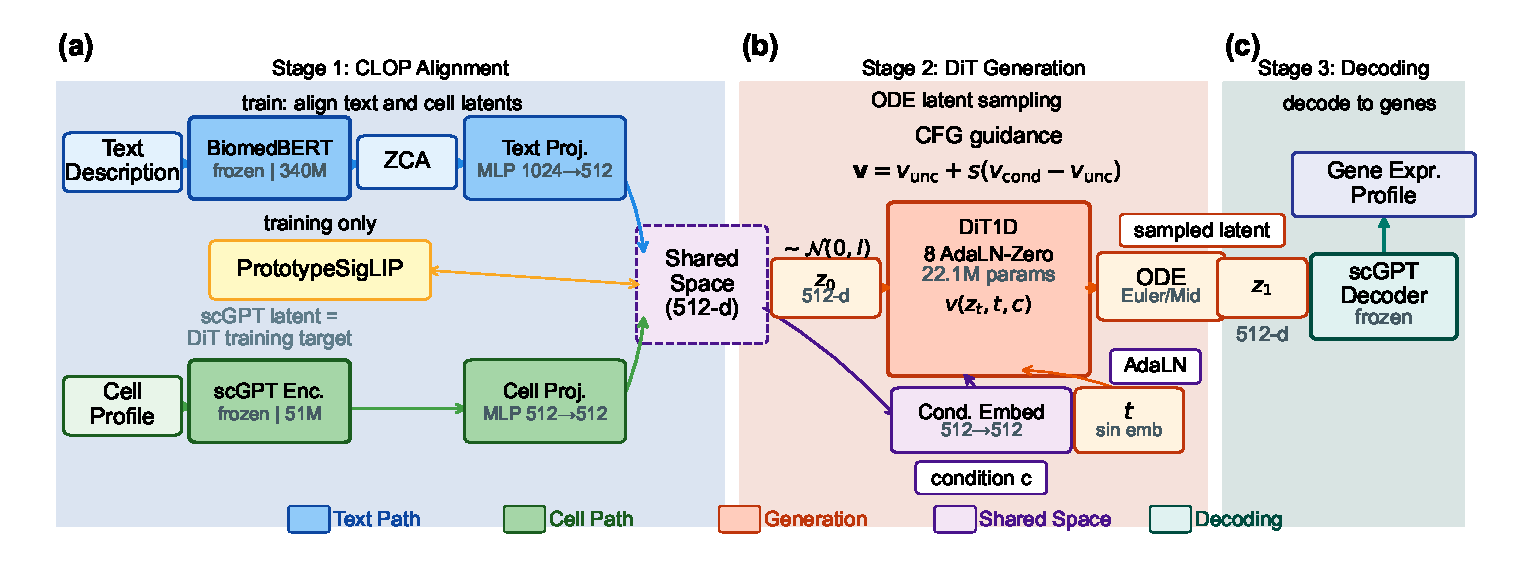
\includegraphics[width=\textwidth]{figures/fig01a_architecture.pdf}\par\vspace{-2pt}
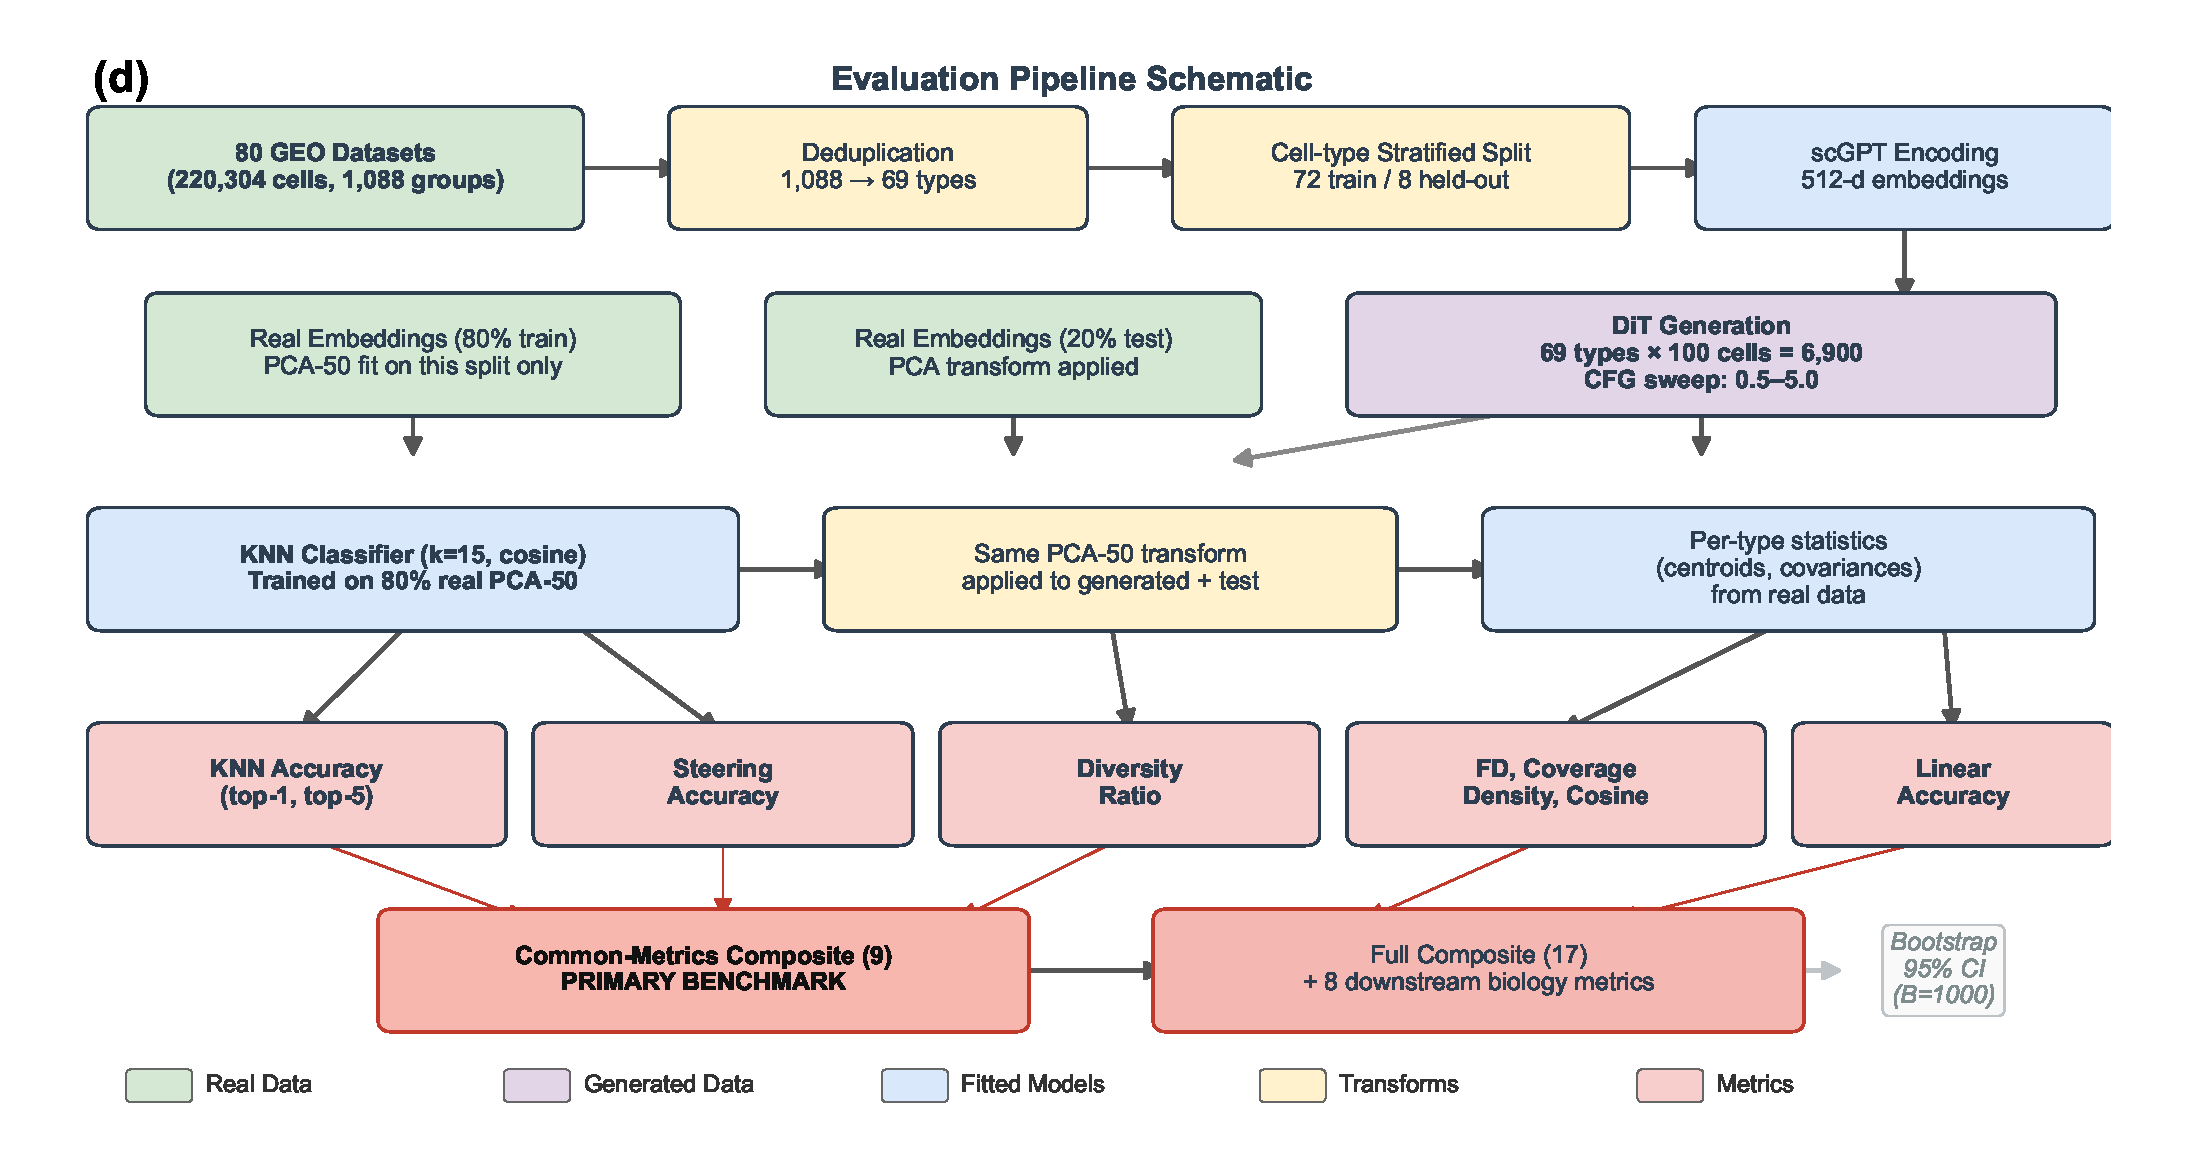
\includegraphics[width=0.95\textwidth]{figures/fig01b_evaluation_pipeline.pdf}
\caption{\textbf{CLOP-DiT pipeline overview and evaluation framework.} \textbf{(Top)} \textbf{Stage~1 (CLOP)} aligns structured text descriptions and scGPT cell embeddings in a shared 512-dimensional space after BiomedBERT whitening and projection. \textbf{Stage~2 (DiT)} performs conditional flow matching in scGPT latent space and generates a target latent from Gaussian noise using classifier-free guidance at inference. \textbf{Stage~3 (Decoding)} maps the generated latent back to gene expression through the frozen scGPT decoder. \textbf{(Bottom)} Evaluation pipeline schematic: data flow from raw datasets through deduplication, stratified splitting, scGPT encoding, PCA fitting (on real training split only), KNN classifier training, and metric computation. The common-metrics-only composite (9 shared distributional metrics) is the primary benchmark; bootstrap confidence intervals ($B{=}1{,}000$) are computed by resampling the 69 evaluation types.\label{fig:architecture}\label{fig:eval-pipeline}}
\end{figure}

\subsection{Datasets and preprocessing}\label{sec:dataset}

We curated 80 scRNA-seq datasets from the Gene Expression Omnibus (GEO), spanning cancer and developmental biology and totaling 220,304 cells after quality control and highly variable gene selection~\citep{ref-seurat,ref-hvg}. For each dataset, 2,000 highly variable genes were retained. Each cell was then encoded as a 512-dimensional embedding by a pre-trained scGPT model. Cell-type annotations were organized into 1,088 unique text groups, each represented by a structured caption rather than free-form prose. These captions combine cell type, marker genes, tissue of origin, organism, and disease context using the following template:
\begin{quote}\small\ttfamily
\{cell type\}, tissue: \{tissue\}, organism: \{organism\},\\
markers: \{top 5 DE marker genes\}, context: \{disease/condition\}
\end{quote}
\noindent Marker genes were identified by one-vs.-rest Wilcoxon rank-sum testing on the training split~\citep{ref-wilcoxon}. To check that these markers were not merely circular artifacts of the training corpus, we compared them against PanglaoDB~\citep{ref-panglao} and CellMarker~2.0~\citep{ref-cellmarker}. The resulting Jaccard overlap (0.39--0.45, well above the ${\sim}$0.01 expected for random gene sets of this size) indicates substantial agreement with external biological knowledge (see Discussion). The exact caption template and marker-gene sources are provided in the project repository~\citep{ref-clop-dit}.

Before CLOP training, both BiomedBERT text embeddings and scGPT cell embeddings were preprocessed upstream by mean-centering, ZCA whitening, and $L_2$ normalization using statistics estimated from the training data. Text preprocessing was fit on unique captions to avoid overweighting duplicated descriptions, whereas cell preprocessing was fit on a 50,000-cell training subsample for efficiency and then applied to the full corpus. As a result, the contrastive aligner operates on preprocessed encoder outputs rather than learning whitening inside the network.

The corpus was split into 72 training datasets (199,670 cells) and 8 held-out validation datasets (20,634 cells). Validation was defined at the study level rather than the cell level so that no samples overlap between training and validation. The held-out studies were chosen by stratified selection across the major tissue and cancer categories represented in the corpus (lung, gastric, skin, liver, blood). The full list of 80 GEO accession identifiers is provided in Table~\ref{tab:s1_datasets} (Appendix~\ref{app:suppl-tables}), and the validation studies are listed in Table~\ref{tab:s2_validation}. Within the training studies, a cell-type-stratified split reserves approximately 10\% of cells per type for training-time validation, ensuring that all 69 deduplicated evaluation types are represented in both partitions. This design therefore tests interpolation within the observed training distribution rather than stringent out-of-distribution generalization.

The relationship between the 1,088 text groups and the 69 evaluated cell types is as follows. The 1,088 text groups correspond to sub-cluster-level descriptions: each Leiden~\citep{ref-leiden} cluster within each dataset receives its own caption. Many sub-clusters nevertheless map to the same canonical cell type (for example, ``CD8+ T cells'' appearing in distinct tissues or studies). For evaluation, these text groups are consolidated by core identity through a deduplication pipeline that (a)~removes ambiguous or uncharacterized sub-clusters and (b)~merges cross-dataset sub-clusters into canonical types, yielding 69 evaluable cell types. The resulting deduplicated cache contains 167,245 cells and is the basis for all headline generation metrics, bootstrap confidence intervals, and benchmark comparisons. KNN accuracy is therefore reported over a consistent 69-type problem (random chance = $1/69 \approx 1.45\%$).

The 80 datasets include both \textit{Homo sapiens} (59 datasets) and \textit{Mus musculus} (21 datasets, including Tabula Muris~\citep{ref-tabula-muris}) and are dominated by tumor-microenvironment and developmental contexts. All claims in this study should therefore be interpreted within that scope; generalization to other organisms, non-cancer tissues, or perturbation-heavy settings has not been tested. Training and evaluation were implemented in Python~3.10 using PyTorch~2.1 (CUDA~12.0), scGPT~v0.2.1, and Hugging Face Transformers~4.36 for BiomedBERT; the complete environment specification is available in the project repository~\citep{ref-clop-dit}.

\paragraph{Hardware and compute budget.}
All training and evaluation were conducted on a single NVIDIA GeForce RTX~5090 Laptop GPU (24\,GB VRAM) using PyTorch~2.1 with CUDA~12.0 and automatic mixed precision (AMP/FP16). The total compute budget remains modest ($<$2 GPU-hours in aggregate, $<$24\,GB VRAM peak), so reproduction should be feasible on any Ampere-or-later GPU with at least 16\,GB VRAM. CLOP alignment training completes in minutes, DiT training in roughly an hour-scale run, and end-to-end figure regeneration from cached embeddings in under 30~minutes. No multi-GPU or distributed training was used. Inference for 69 cell types (approximately 6,900 generated cells) takes about 2~minutes with 10-step Euler integration.

\subsection{CLOP: Contrastive Language--Omics Pretraining}\label{sec:clop}

CLOP aligns structured metadata descriptions and cell profiles in a shared 512-dimensional embedding space, producing the condition representation used by the DiT. A frozen BiomedBERT-large encoder maps captions to 1024-dimensional embeddings, and a frozen scGPT encoder maps cells to 512-dimensional embeddings. The production aligner uses dual three-layer MLP projectors (text: $1024 \to 1024 \to 1024 \to 512$; cell: $512 \to 512 \to 512 \to 512$) with LayerNorm, GELU activation~\citep{ref-gelu}, and dropout~\citep{ref-dropout} (0.2), followed by $L_2$ normalization onto the unit hypersphere. In the final configuration, duplicate captions within a mini-batch are masked so that cells sharing the same caption are not treated as false negatives.

Because many cells share the same caption, the production objective is not a pure instance-level cross-entropy loss. Instead, CLOP uses a PrototypeSigLIP loss that aligns one representative text projection per caption group to the centroid of the corresponding cell projections within the batch. Let $S_g$ denote the set of cells in group $g$, $\mathbf{c}_i$ the projected cell embedding of cell $i$, and
\begin{equation}
\mathbf{p}_g = \mathrm{norm}\!\left(\frac{1}{|S_g|}\sum_{i \in S_g} \mathbf{c}_i\right)
\end{equation}
the normalized prototype for that group. With representative text projection $\mathbf{t}_g$, learned bias $b$, and fixed logit scale $\tau$, the prototype-alignment term is
\begin{equation}
\ell_{gh} = \tau\,\mathbf{t}_g^\top \mathbf{p}_h + b, \qquad
\mathcal{L}_\text{align} = -\frac{1}{G^2}\sum_{g=1}^{G}\sum_{h=1}^{G}\log\sigma\!\left(y_{gh}\,\ell_{gh}\right),
\label{eq:clop}
\end{equation}
where $y_{gh}=1$ when $g=h$ and $y_{gh}=-1$ otherwise, $G$ is the number of caption groups in the batch, and $\sigma(\cdot)$ is the sigmoid function. A cohesion penalty then pulls individual cell projections toward their group prototype:
\begin{equation}
\mathcal{L}_\text{CLOP} = \mathcal{L}_\text{align} + \lambda_\text{coh}\,\frac{1}{B}\sum_{i=1}^{B}\left(1 - \mathbf{c}_i^\top \mathrm{sg}(\mathbf{p}_{g(i)})\right),
\end{equation}
with $\lambda_\text{coh}=0.15$, batch size $B$, and $\mathrm{sg}(\cdot)$ denoting stop-gradient. In the production configuration, the SigLIP logit scale is fixed at $\tau = 14.0$ rather than learned. The aligner has 3.02M trainable parameters and is optimized with AdamW~\citep{ref-adamw} (lr~$= 5 \times 10^{-4}$, weight decay 0.06, cosine schedule~\citep{ref-cosine-schedule} with 5-epoch warmup) over a 100-epoch training run.

The key output of CLOP is the projected condition space. Raw scGPT cell-type centroids have a mean pairwise cosine similarity of 0.994 (that is, cell types differ by only 0.6\% on average), whereas CLOP-projected conditions reduce this mean to 0.222, increasing inter-group separation by approximately $130\times$. That improvement is what makes conditional generation in the subsequent DiT stage feasible.

\subsection{DiT: Conditional Flow Matching with Diffusion Transformer}\label{sec:dit}

The Diffusion Transformer (DiT1D) reshapes each 512-dimensional cell embedding into 16 pseudo-tokens of dimension 32. The backbone comprises 8 AdaLN-Zero transformer blocks with 8-head self-attention and an MLP expansion ratio of 4.0, corresponding to feed-forward sublayers of size $512 \to 2048 \to 512$. Timestep information and CLOP condition vectors are each projected to 512 dimensions and combined by element-wise summation, so every block is modulated by a shared conditioning signal rather than by concatenated inputs. The model has 22.10M trainable parameters (Table~\ref{tab:architecture}).

The base training objective is the standard flow-matching loss~\citep{ref-flow-matching,ref-ot-cfm}:
\begin{equation}
\mathcal{L}_\text{FM} = \| v_\theta(z_t, t, c) - (z_1 - z_0) \|_2^2,
\label{eq:fm}
\end{equation}
where $z_0 \sim \mathcal{N}(0, I)$, $z_1$ is the real cell embedding, $z_t = (1-t)z_0 + tz_1$, and $t$ is drawn from a logit-normal distribution ($\mu{=}0, \sigma{=}1$), which concentrates training on intermediate timesteps where the velocity field is most complex~\citep{ref-sd3}. During training, classifier-free guidance (CFG)~\citep{ref-cfg} is implemented by dropping the condition with 15\% probability and replacing it with a \emph{learned} null condition token. At inference,
\begin{equation}
v_\text{guided} = v_\text{uncond} + s \cdot (v_\text{cond} - v_\text{uncond}),
\label{eq:cfg}
\end{equation}
where $s$ is the guidance scale.

To reduce mean-collapse, the production DiT adds two group-aware regularizers on the reconstructed clean latent $\hat{z}_1 = z_t + (1-t)\,v_\theta(z_t,t,c)$: a per-group variance-matching term and a sliced covariance-matching term based on random one-dimensional projections. The full objective is therefore
\begin{equation}
\mathcal{L}_\text{DiT} = \mathcal{L}_\text{FM} + \lambda_\text{var}\,\mathcal{L}_\text{var} + \lambda_\text{cov}\,\mathcal{L}_\text{cov},
\label{eq:var-loss}
\end{equation}
with $\lambda_\text{var}=0.10$ and $\lambda_\text{cov}=0.05$. Here, $\mathcal{L}_\text{var}$ matches per-dimension variance within each caption group, and $\mathcal{L}_\text{cov}$ matches the variance of random projected views of real and reconstructed clean latents, providing a sliced approximation to covariance preservation. DiT is optimized with AdamW for a 300-epoch training run using EMA~\citep{ref-ema} (decay = 0.9999), cosine learning-rate decay with 5-epoch warmup, AMP, and gradient clipping at 1.0.

\subsection{Decoding via scGPT}\label{sec:decoding}

Generated latent vectors $z_1 \in \mathbb{R}^{512}$ are mapped back to gene expression using the frozen scGPT decoder. This stage is useful for downstream biological inspection, but it also imposes an important limitation: the decoder is many-to-one, so distinct latents near the training manifold can decode to similar expression profiles. We therefore treat latent-space metrics---KNN accuracy, steering, diversity ratio, and centroid cosine---as the primary indicators of generative quality, whereas expression-space analyses are interpreted as compatibility checks on the full pipeline rather than as direct measures of latent fidelity. Relaxing this bottleneck will require either decoder fine-tuning or a lightweight trainable adapter.

\subsection{Evaluation Framework}\label{sec:evaluation}

We evaluate CLOP-DiT along six axes using in-distribution conditions (the actual CLOP-projected text embeddings from training data):

\begin{enumerate}[noitemsep]
\item \textbf{KNN classification accuracy}: For each generated cell, a $k$-nearest-neighbor classifier ($k{=}15$, cosine metric, PCA-50 features) trained on 80\% of real data predicts its cell type. PCA is fitted on the real training split only and applied identically to generated embeddings; the same PCA transform is used across all method comparisons. Random chance is $1/69 \approx 1.45\%$. Because real cell-type centroids in scGPT space have pairwise cosine similarity of 0.994, small embedding perturbations can substantially affect KNN accuracy; the biological meaning of absolute KNN values therefore warrants caution.
\item \textbf{Steering accuracy}: For random cell-type pairs $(A, B)$, we generate cells conditioned on $A$ and test whether the generated centroid is closer to the real cluster $A$ than $B$ in centered space. Random chance is 50\%. \textbf{Note:} At intermediate-to-high CFG values (e.g., CFG$\,\geq\,$1.5) with multi-step solvers, steering accuracy can saturate at 1.0 with bootstrap CI [1.0, 1.0], indicating a ceiling effect; this metric loses discriminative power once guidance is sufficient.
\item \textbf{Diversity ratio}: Ratio of generated within-group variance to real within-group variance. Ideal is 1.0; values $<$1 indicate mode sharpening; values $>$1 indicate excess noise.
\item \textbf{Coverage and density}: Coverage measures the fraction of real samples that have at least one generated neighbor within the real data's KNN radius ($k{=}5$); it quantifies mode coverage. Density measures the average number of generated samples falling within each real sample's KNN radius, normalised by $k$; it quantifies precision. Both are computed in PCA-50 embedding space.
\item \textbf{Centroid cosine similarity}: The cosine similarity between the real and generated cell-type centroids, computed in the 512-dimensional scGPT embedding space (uncentered; $\text{cos}(\boldsymbol{\mu}_\text{real}, \boldsymbol{\mu}_\text{gen})$). Reported per-type and averaged across 69 types.
\item \textbf{Downstream biological concordance}: Clustering alignment (ARI~\citep{ref-ari}, NMI~\citep{ref-nmi}), classifier transfer, and differential expression concordance between real and generated data.
\end{enumerate}

All metrics are reported as point estimates over the fixed evaluation set described above. Two configurations are designated as \emph{primary operating points}: CFG\,=\,2.0 with 10-step Euler integration (high-fidelity regime) and CFG\,=\,1.0 with 10-step Midpoint integration (high-diversity regime). All other CFG and solver combinations in Appendix~\ref{app:suppl-tables} represent sensitivity analysis; no multiple-comparison correction was applied to these exploratory comparisons. Bootstrap 95\% confidence intervals for the composite benchmark scores are shown in Figure~\ref{fig:benchmark}d; variability across single-measurement metrics (KNN, steering, diversity ratio) is characterized by the CFG sweep (Appendix~\ref{app:suppl-tables}, Table~\ref{tab:cfg-sweep}).

\textbf{Caveat on Fr\'{e}chet Distance (FD).} FD~\citep{ref-fid} compares distributional moments (mean and covariance) between real and generated samples. While widely used for unconditional evaluation, FD can be misleading for \emph{conditional} generation: a model that reproduces the global marginal distribution but ignores conditioning achieves a low FD without having learned the target conditional. FD is therefore reported as a secondary metric throughout; the primary metrics (KNN accuracy, steering, diversity ratio) are specifically designed for conditional evaluation.

The biological evidence is organized by figure family: Figures~\ref{fig:markers}--\ref{fig:expr-analysis} establish marker-level and gene-level fidelity; Figures~\ref{fig:diversity} and~\ref{fig:expr-diversity} provide robustness readouts for guidance and diversity; Figure~\ref{fig:baselines} reports benchmarking; Figure~\ref{fig:downstream-pq} tests downstream biology. The evaluation pipeline is shown in the bottom panel of Figure~\ref{fig:eval-pipeline}.

Having established the methodology and evaluation framework, we now present the empirical results.

\subsection{Statistical Analysis}\label{sec:stats}

\textbf{Primary endpoints.} Two operating points were pre-specified as primary comparisons: CFG\,=\,2.0 with 10-step Euler integration (high-fidelity regime, selected because KNN accuracy plateaus at CFG 2.0--3.0 in Table~\ref{tab:cfg-sweep}; the lower end was chosen to minimize diversity loss) and CFG\,=\,1.0 with 10-step Midpoint integration (high-diversity regime, selected to match DivR\,$\approx$\,1.0). The primary metrics are KNN top-1 classification accuracy (69-class, $k{=}15$, cosine metric on PCA-50 features) and steering accuracy (pairwise directional test, 1000 random pairs).

\textbf{Exploratory analyses.} All other CFG/solver/step combinations reported in Tables~\ref{tab:cfg-sweep} and~\ref{tab:s3_cfg_sweep} (Appendix~\ref{app:suppl-tables}) constitute exploratory sensitivity analyses. No correction for multiple comparisons (e.g., Bonferroni, Holm) was applied to these comparisons. Rankings and performance claims refer only to the two primary operating points unless explicitly stated otherwise.

\textbf{Uncertainty quantification.} Bootstrap 95\% confidence intervals (percentile method, $B{=}1000$ resamples, seed 42) are reported for all headline metrics where per-unit (per-cell or per-type) data are available (see Results). These CIs capture evaluation sampling variability but not training-run variance, as all results derive from a single training run (seed 42). Formal superiority tests (e.g., permutation tests) were not conducted; all comparisons are descriptive.

\textbf{Multi-seed replication.} To characterize inter-run variance, we trained three independent CLOP + DiT pipeline replicas (seeds 42, 123, 456) with identical hyperparameters and report mean $\pm$ standard deviation for all core metrics in Table~\ref{tab:multi-seed} (see Section~\ref{sec:multi-seed-results}).

\textbf{Limitations of the statistical design.} (1)~No formal pre-registration: operating points were selected based on interpretable criteria post-hoc rather than by pre-registered protocol; this study is therefore exploratory rather than confirmatory. (2)~No multiple-comparison correction for the exploratory CFG sweep.

\subsection{Composite Score Formulation}\label{sec:composite}

The composite benchmark score aggregates all active metrics into a single ranking index. For each metric~$m$ with direction $d_m \in \{\text{lower}, \text{higher}\}$, let $v_{m,j}$ denote the raw value for method~$j$. We compute a min--max normalised score:
\begin{equation}
  s_{m,j} =
  \begin{cases}
    1 - \dfrac{v_{m,j} - \min_k v_{m,k}}{\max_k v_{m,k} - \min_k v_{m,k}} & \text{if } d_m = \text{lower},\\[6pt]
    \dfrac{v_{m,j} - \min_k v_{m,k}}{\max_k v_{m,k} - \min_k v_{m,k}} & \text{if } d_m = \text{higher},
  \end{cases}
  \label{eq:norm}
\end{equation}
where $k$ ranges over all methods that report a non-null value for~$m$; methods lacking metric~$m$ receive $s_{m,j} = 0$. The composite score is the unweighted arithmetic mean over all~$M$ active metrics:
\begin{equation}
  C_j = \frac{1}{M}\sum_{m=1}^{M} s_{m,j}.
  \label{eq:composite}
\end{equation}
Because not all methods support downstream biology (Section~\ref{sec:evaluation}, axis~6), they receive $s = 0$ on those metrics, which inflates the score of methods that do. In the current benchmark, 8 of 17 active metrics are reported only by CLOP-DiT; the remaining 9 distributional metrics are shared by all methods. \textbf{To enable fair like-for-like comparison, the common-metrics-only composite ($C_j^{\text{common}}$, restricted to the 9 shared distributional metrics) serves as the primary benchmark figure.} The full composite ($C_j$ over all $M = 17$ metrics) is reported as a supplementary capability ranking but should not be used for method comparison, as the 8 exclusive metrics structurally bias it in favor of CLOP-DiT. Table~\ref{tab:core-results} and the per-metric panels in Figure~\ref{fig:benchmark} report individual metrics for transparent comparison. Bootstrap 95\% confidence intervals (percentile method, $B{=}1{,}000$) for all headline generation metrics are provided in Table~\ref{tab:s5_bootstrap_ci} (Appendix~\ref{app:suppl-tables}).

\section{Results}\label{sec:results}

We report in-distribution results along the six evaluation axes defined in the Methods, organized by evidence type:
training dynamics and embedding space (Figure~\ref{fig:training});
core generation quality metrics and per-type analysis (Figure~\ref{fig:metrics});
gene-level fidelity (Figures~\ref{fig:markers}--\ref{fig:expr-analysis});
conditioning robustness and diversity trade-offs (Figures~\ref{fig:cond-umap},~\ref{fig:diversity}, and~\ref{fig:expr-diversity});
baseline comparisons and benchmarking (Figure~\ref{fig:baselines});
and downstream biological validation (Figure~\ref{fig:downstream-pq}).
This structure allows readers to assess evidence quality at multiple resolutions, from training convergence through partial downstream biological utility.

\subsection{Training Dynamics and Embedding Space}

Figure~\ref{fig:training} summarizes convergence across the two training stages. CLOP rapidly reduces alignment loss and steadily improves prototype-level separation, indicating that the whitened encoder embeddings and LayerNorm-based projectors yield a stable condition space rather than a collapsed contrastive solution. DiT training is similarly well behaved: validation velocity cosine rises sharply early and then improves more gradually under EMA averaging, consistent with reliable learning of the conditional velocity field.

The embedding visualizations (panels i--n) show the geometry induced by this pipeline. In the CLOP shared space, text and cell embeddings co-localize by cell type while remaining well separated across types, confirming successful cross-modal alignment. In scGPT latent space, generated cells overlap substantially with the corresponding real populations but do not collapse onto them, indicating that conditional flow matching captures type-specific structure while still preserving stochastic variation from the noise initialization $z_0 \sim \mathcal{N}(0,I)$.

\begin{figure}[!htbp]
\centering
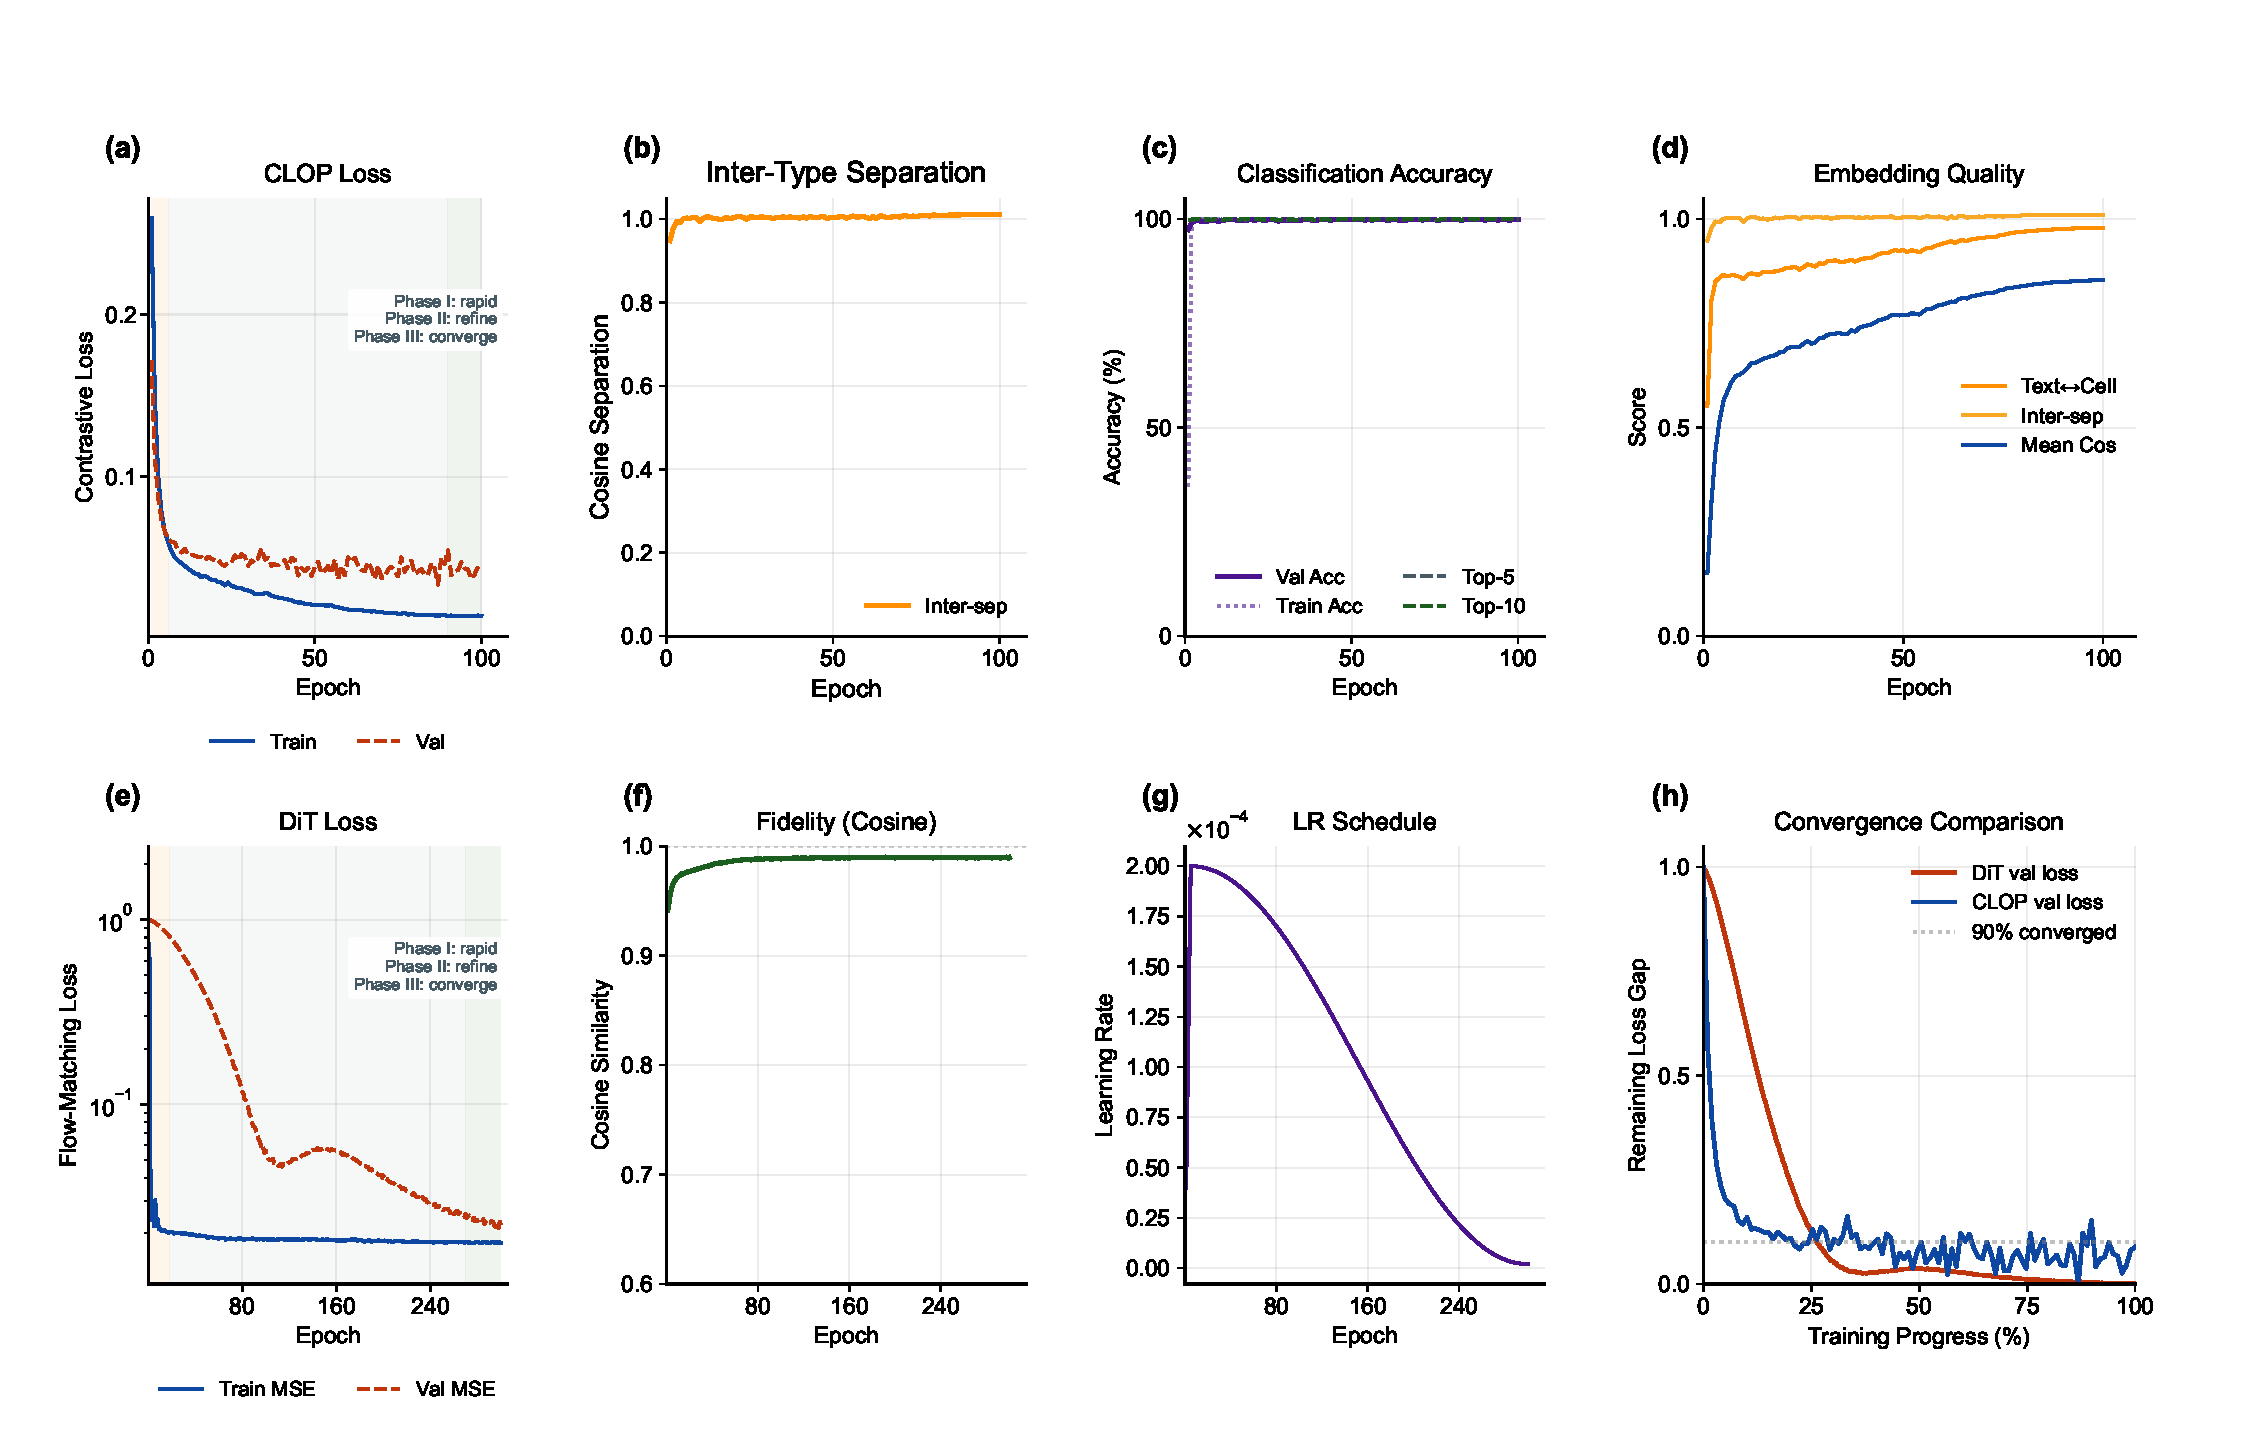
\includegraphics[width=0.95\textwidth]{figures/fig02a_training_dynamics.pdf}\par\vspace{-4pt}
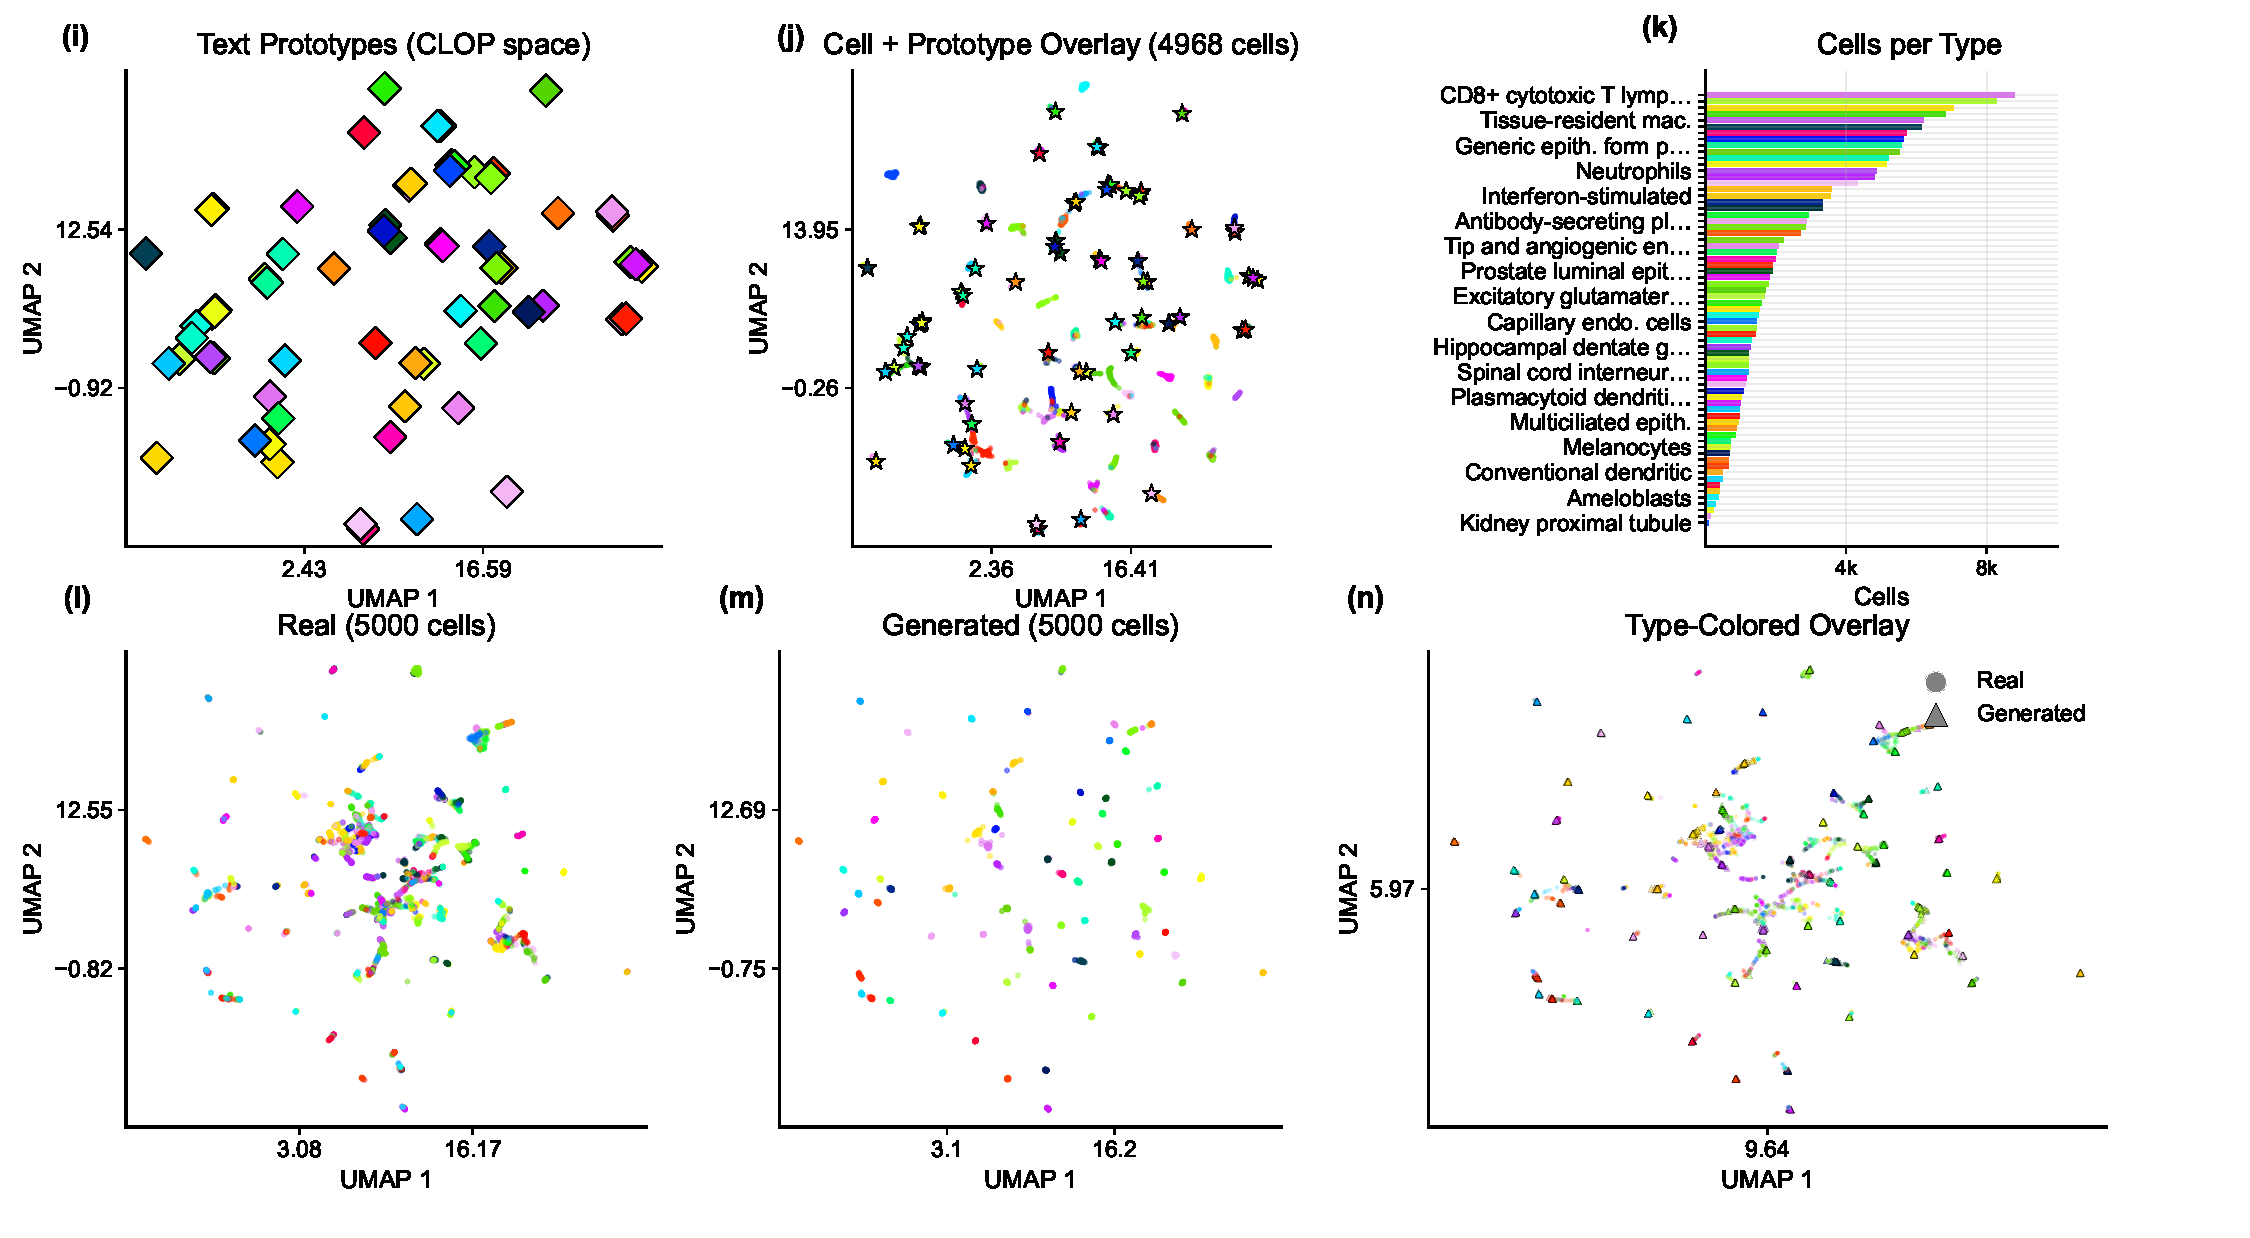
\includegraphics[width=0.95\textwidth]{figures/fig02b_embedding_space.pdf}
\caption{\textbf{Training dynamics and embedding space analysis.} \emph{Training dynamics} (\textbf{a--d})~CLOP loss, inter-type cosine separation, batch accuracy, and embedding-quality metrics over the reported training run. (\textbf{e--h})~DiT train/validation loss, velocity cosine similarity, learning-rate schedule, and normalized convergence comparison. \emph{Embedding space} (\textbf{i--j})~CLOP-projected text and cell embeddings form aligned clusters in the shared space. (\textbf{k})~Cell-count distribution across types. (\textbf{l--n})~Real and generated scGPT embeddings occupy overlapping but distinguishable regions.\label{fig:training}\label{fig:embedding-space}}
\end{figure}

\subsection{Core Evaluation Metrics}

Table~\ref{tab:core-results} and Figure~\ref{fig:metrics} summarize performance across representative generation settings. In the high-fidelity regime (CFG = 2.0, 10-step Euler), CLOP-DiT achieves a KNN top-1 accuracy of 36.9\% ($25\times$ random chance of 1.45\%; 52 percentage points below the 89\% real-data baseline), KNN top-5 of 55.3\%, steering accuracy of 81.0\%, and linear classifier accuracy of 51.1\%. The unconditional control ($s{=}0$) collapses to chance-level type specificity (KNN = 1.0\%, steering = 47.5\%), confirming that prompt conditioning rather than the sampler or decoder alone drives the observed structure. Fr\'{e}chet distance (FD) is reported for completeness, but because it rewards global moment matching even when conditioning is ignored, we interpret it only as a secondary distributional diagnostic.

\begin{table}[!htbp]
\caption{Core evaluation results. KNN-1 and KNN-5: top-1 and top-5 $k$-nearest-neighbor accuracy among 69 deduplicated cell types (random = 1.45\%). Steering: pairwise directional accuracy (random = 50\%). DivR: diversity ratio with ideal = 1.0. LinAcc: logistic regression accuracy in embedding space (trained on real, evaluated on generated; distinct from the expression-space downstream classifier in Figure~\ref{fig:downstream-pq}). FD: Fr\'{e}chet distance~\citep{ref-fid} (lower is better, but misleading for conditional generation; see text).\label{tab:core-results}}
\centering
\begin{tabularx}{\textwidth}{lCCCCCC}
\toprule
\textbf{Method} & \textbf{KNN-1} & \textbf{KNN-5} & \textbf{Steering} & \textbf{DivR} & \textbf{LinAcc} & \textbf{FD} \\
\midrule
Real data        & 0.890 & 0.993 & ---   & 1.000 & 0.942 & 0.00 \\
CFG=2.0 Euler-10 & 0.369 & 0.553 & 0.810 & 0.513 & 0.511 & 3.17 \\
CFG=3.0 Euler-10 & 0.367 & 0.554 & 0.802 & 0.473 & 0.508 & 3.46 \\
CFG=1.0 Mid-10   & 0.288 & 0.461 & 0.807 & 0.929 & 0.357 & 2.64 \\
CFG=1.0 Euler-50 & 0.293 & 0.466 & 0.807 & 0.919 & 0.365 & 2.65 \\
CFG=0.0 (uncond) & 0.010 & 0.051 & 0.475 & 1.833 & 0.010 & 0.58 \\
Gaussian          & 0.011 & 0.048 & 0.466 & 2.277 & 0.009 & 0.03 \\
\midrule
Random chance    & 0.010 & ---   & 0.500 & ---   & ---   & ---  \\
\bottomrule
\end{tabularx}
\end{table}

\begin{figure}[!htbp]
\centering
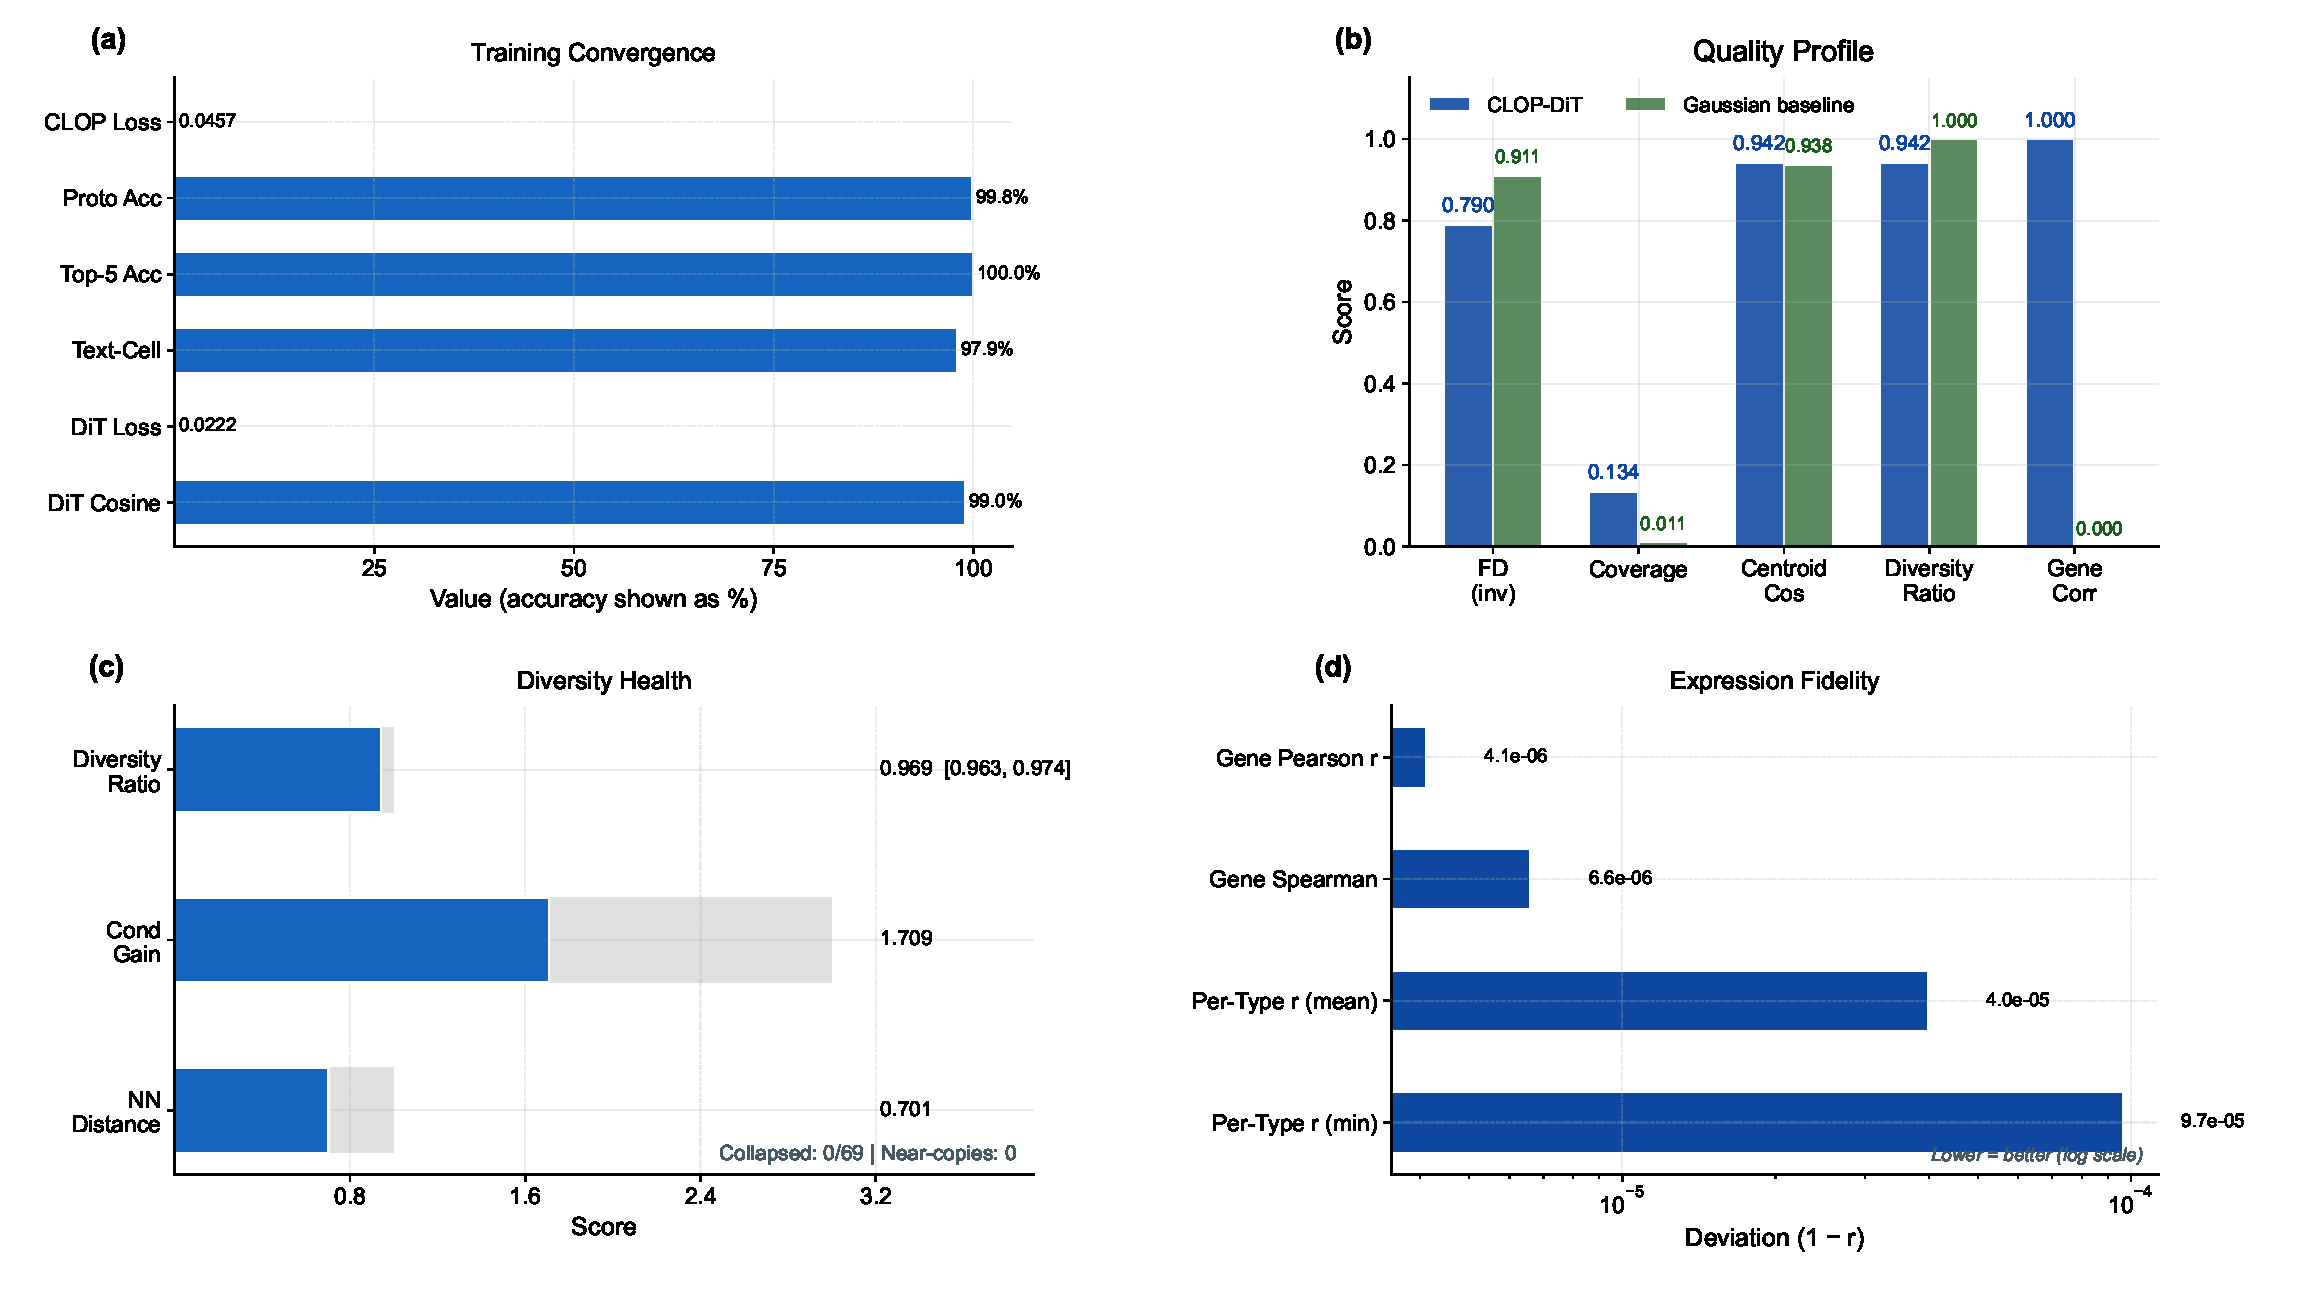
\includegraphics[width=0.95\textwidth]{figures/fig03a_metrics_summary.pdf}\par\vspace{0pt}
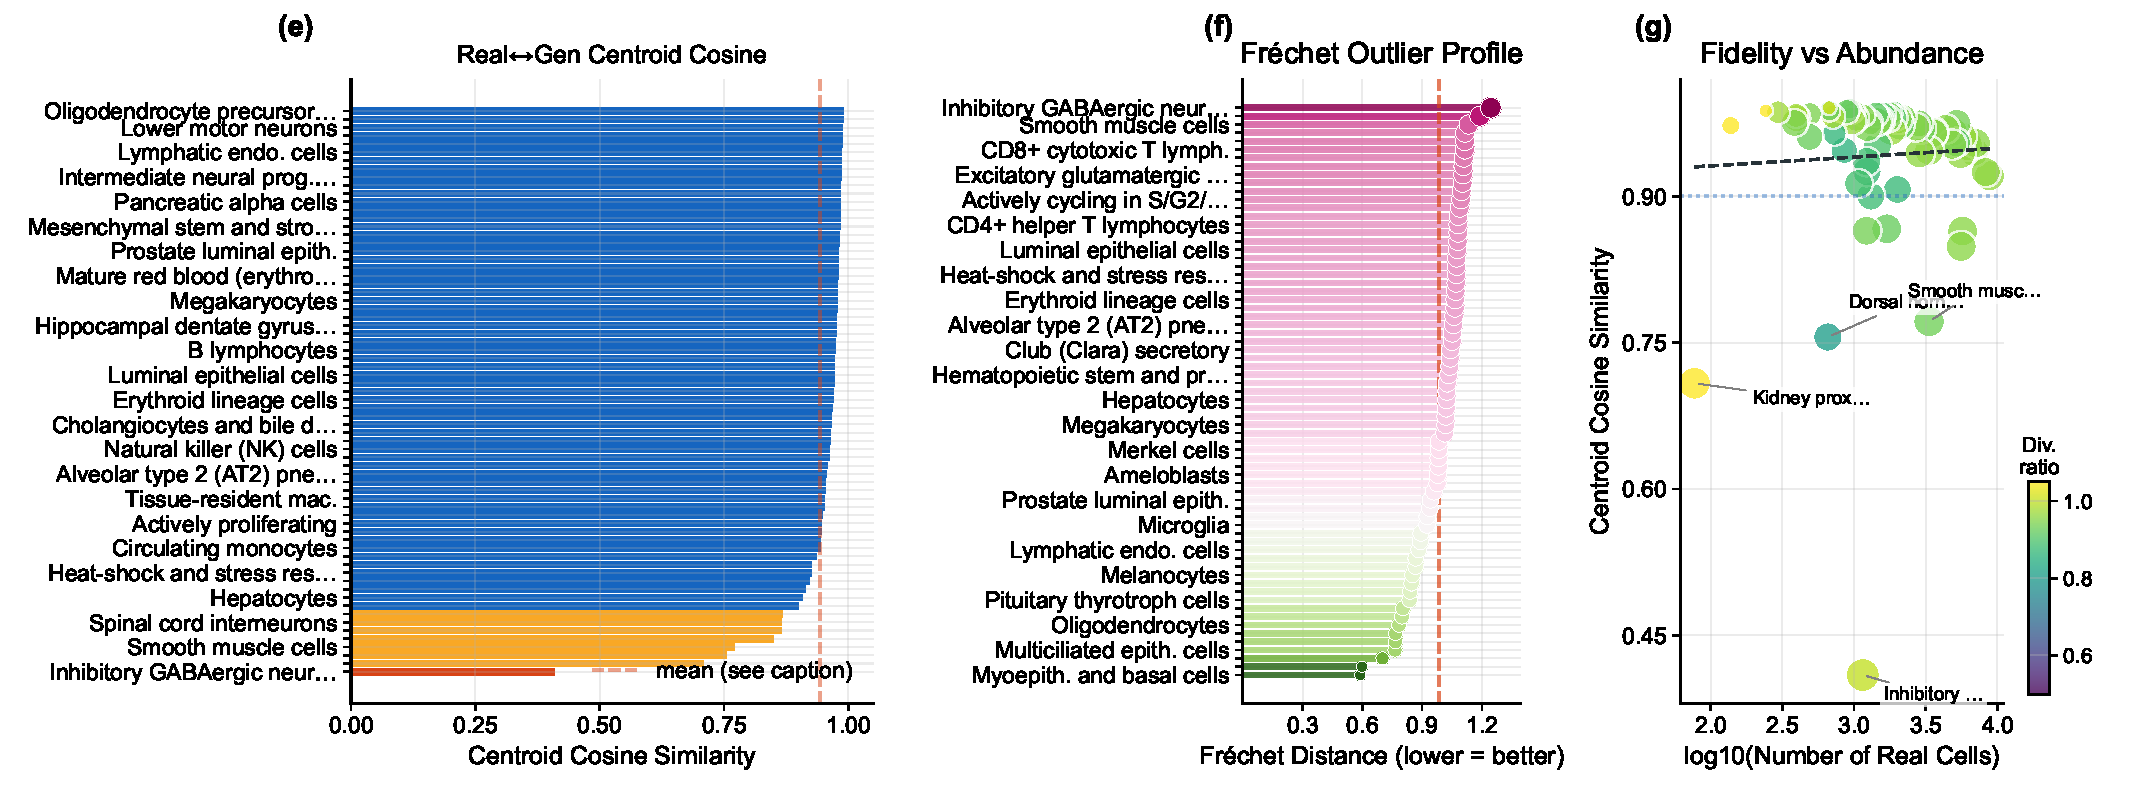
\includegraphics[width=0.95\textwidth]{figures/fig03b_per_type_fidelity.pdf}\par\vspace{0pt}
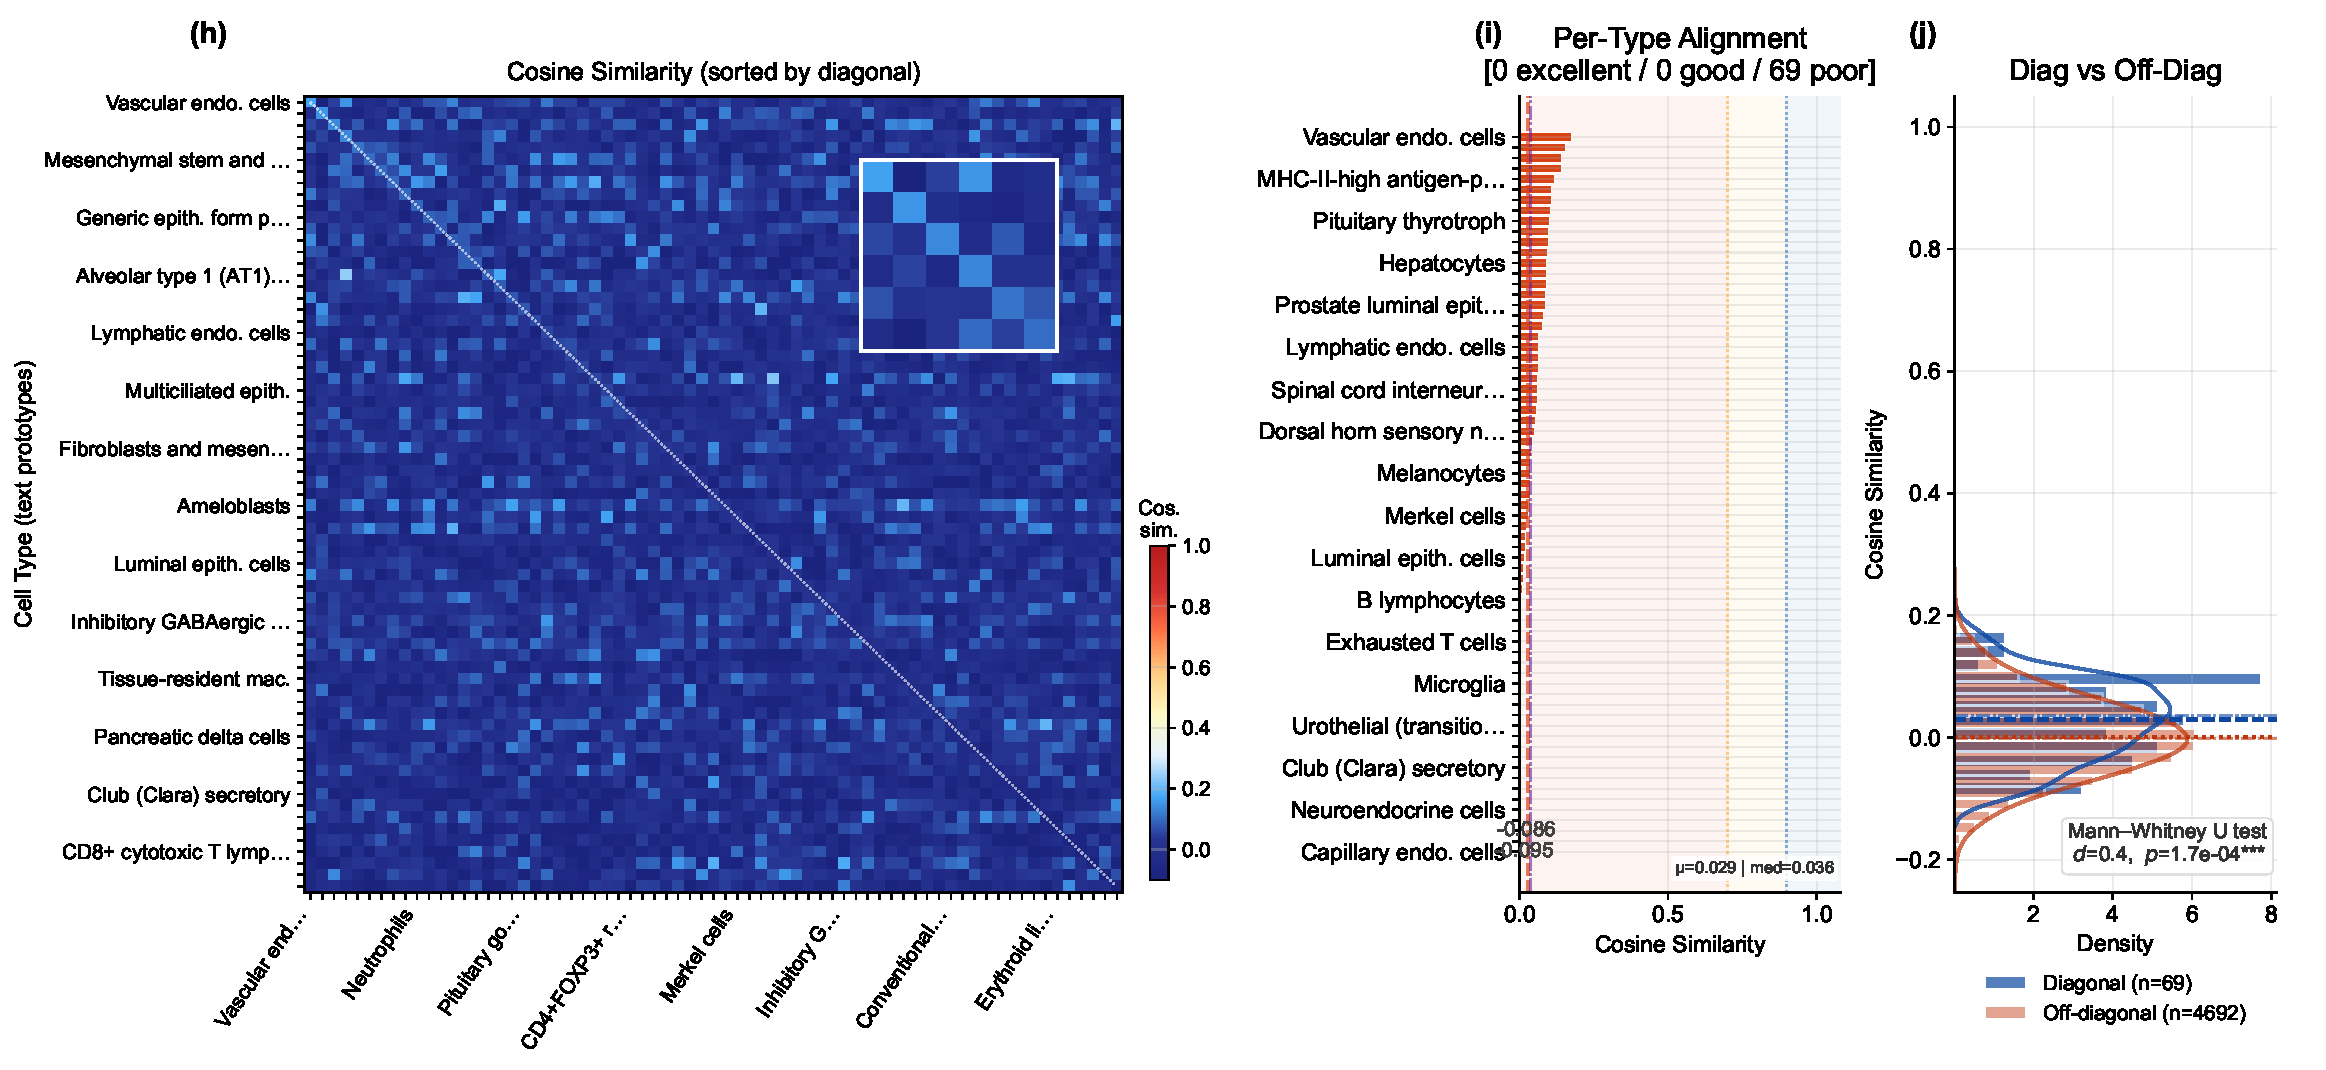
\includegraphics[width=0.95\textwidth]{figures/fig03c_text_cell_alignment.pdf}
\caption{\textbf{Generation quality overview: metrics, per-type fidelity, and text--cell alignment.} \emph{Metrics dashboard} (\textbf{a})~Training convergence summary. (\textbf{b})~Multi-metric comparison between CLOP-DiT and the Gaussian baseline. (\textbf{c})~Diversity health gauges. (\textbf{d})~Expression-fidelity deviation ($1 - r$, log scale). \emph{Per-type fidelity} (\textbf{e})~Per-type centroid cosine similarity ranked across cell types, (\textbf{f})~Fr\'{e}chet outlier profile, and (\textbf{g})~abundance--fidelity scatter. \emph{Text--cell alignment} (\textbf{h})~69$\times$69 cosine similarity heatmap (mean diagonal $\mu_{\text{diag}} = 0.916$, $\sigma = 0.053$; Cohen's $d = 5.8$, separation ratio $20.9\times$). (\textbf{i})~Per-type alignment bars. (\textbf{j})~Diagonal vs.\ off-diagonal distribution comparison ($\Delta = 0.872$, 95\% CI [0.875, 0.913]).\label{fig:metrics}\label{fig:per-type-gen}\label{fig:text-cell-alignment}}
\end{figure}

\textbf{Bootstrap confidence intervals.} To quantify evaluation sampling uncertainty, we computed bootstrap 95\% CIs by resampling the 69 cell types in the generation cache with replacement ($B{=}1{,}000$, percentile method). All 69 deduplicated types have both real and generated cells, so the bootstrap covers the full evaluation set consistently. At an intermediate reference configuration (CFG = 1.5, Midpoint, 20 steps; selected to balance fidelity and diversity between the two primary operating points): KNN top-1 = 0.509 [0.421, 0.586], KNN top-5 = 0.728 [0.658, 0.794], steering = 1.000 [1.000, 1.000] (\textbf{ceiling effect}: all bootstrap resamples achieve perfect pairwise accuracy at this configuration, indicating that the steering metric saturates at moderate-to-high CFG and becomes non-discriminative; this ceiling limits the interpretability of steering differences across configurations), diversity ratio = 0.969 [0.963, 0.974], linear accuracy = 0.583 [0.518, 0.646], and centroid cosine = 0.898 [0.875, 0.913]. The narrow diversity ratio and centroid cosine CIs reflect uniformly high performance across types; the wider KNN CIs reflect type-dependent classification difficulty. These CIs capture evaluation sampling variability; inter-run variance across three training seeds is reported separately in Table~\ref{tab:multi-seed}.

\subsection{Multi-Seed Validation}\label{sec:multi-seed-results}

To quantify inter-run variance from stochastic initialization, data shuffling, and mini-batch ordering, we trained three independent CLOP + DiT pipelines (seeds 42, 123, 456) with identical hyperparameters and evaluated each under both operating regimes (Table~\ref{tab:multi-seed}).

\begin{table}[!htbp]
\caption{Multi-seed validation (3 independent training runs). Mean $\pm$ standard deviation for core metrics under both operating regimes. All three seeds use identical hyperparameters (Table~\ref{tab:hyperparams}), identical data splits, and identical evaluation protocol.\label{tab:multi-seed}}
\centering
\small
\begin{tabular}{lcccc}
\toprule
 & \multicolumn{2}{c}{\textbf{High-Fidelity (CFG=2.0, Euler)}} & \multicolumn{2}{c}{\textbf{High-Diversity (CFG=1.0, Midpoint)}} \\
\cmidrule(lr){2-3}\cmidrule(lr){4-5}
\textbf{Metric} & \textbf{Mean $\pm$ Std} & \textbf{Range} & \textbf{Mean $\pm$ Std} & \textbf{Range} \\
\midrule
KNN Top-1      & $0.348 \pm 0.082$ & [0.258, 0.419] & $0.273 \pm 0.048$ & [0.220, 0.312] \\
KNN Top-5      & $0.535 \pm 0.016$ & [0.524, 0.553] & $0.465 \pm 0.038$ & [0.430, 0.504] \\
Steering       & $0.808 \pm 0.009$ & [0.798, 0.817] & $0.801 \pm 0.008$ & [0.792, 0.807] \\
Diversity Ratio & $0.511 \pm 0.015$ & [0.496, 0.525] & $0.924 \pm 0.016$ & [0.906, 0.937] \\
Linear Acc.    & $0.488 \pm 0.023$ & [0.465, 0.511] & $0.355 \pm 0.097$ & [0.257, 0.452] \\
Centroid Cos.  & $0.892 \pm 0.012$ & [0.878, 0.900] & $0.892 \pm 0.010$ & [0.880, 0.898] \\
\bottomrule
\end{tabular}
\end{table}

Inter-run standard deviations are small relative to effect sizes: steering accuracy varies by $< 1$ percentage point ($\sigma = 0.009$), diversity ratio by $< 2$ percentage points ($\sigma = 0.015$--$0.016$), and centroid cosine by $\sim 1\%$ ($\sigma = 0.010$--$0.012$). KNN top-1 accuracy exhibits the largest inter-seed variance ($\sigma = 0.082$ in the high-fidelity regime), reflecting the sensitivity of nearest-neighbor classification to the decision boundary in the tightly-packed scGPT embedding space. Critically, the qualitative conclusions---$25\times$ above random chance, $\sim$52-point gap from real data, near-ideal diversity at CFG\,=\,1.0---are stable across all three seeds.

\subsection{Per-Type Generation Quality and Text--Cell Alignment}

Beyond aggregate metrics, per-type analysis reveals which cell types benefit most from text conditioning and where failures concentrate. Figure~\ref{fig:per-type-gen} presents per-type generation quality and text--cell alignment. The enhanced per-type analysis now makes heterogeneity explicit: centroid cosine is ranked across all 69 deduplicated cell types; the Fr\'echet profile highlights outlier types rather than only reporting the mean, and the abundance--fidelity scatter encodes Fr\'echet distance as bubble size and diversity ratio as color. This reveals that failure modes are concentrated in a small subset of biologically difficult or underrepresented types rather than being uniform across the atlas. The text--cell alignment analysis (panels h--j) confirms that generated cells remain most similar to their intended text condition despite these type-specific differences.

\subsection{Gene-Level Fidelity}

A key question for conditional generation is whether cell-type-specific marker gene signatures and gene-level expression statistics are preserved. Figure~\ref{fig:gene-fidelity} addresses this at two levels: marker-gene comparison (top) confirms that CLOP-DiT preserves cell-type-specific expression signatures, while per-gene correlation analysis (bottom) localizes fidelity in gene-wise means and marker-level residuals. Figure~\ref{fig:expr-analysis} provides a broader view of expression distribution properties, including per-gene coefficient of variation and per-cell variability.

\begin{figure}[!htbp]
\centering
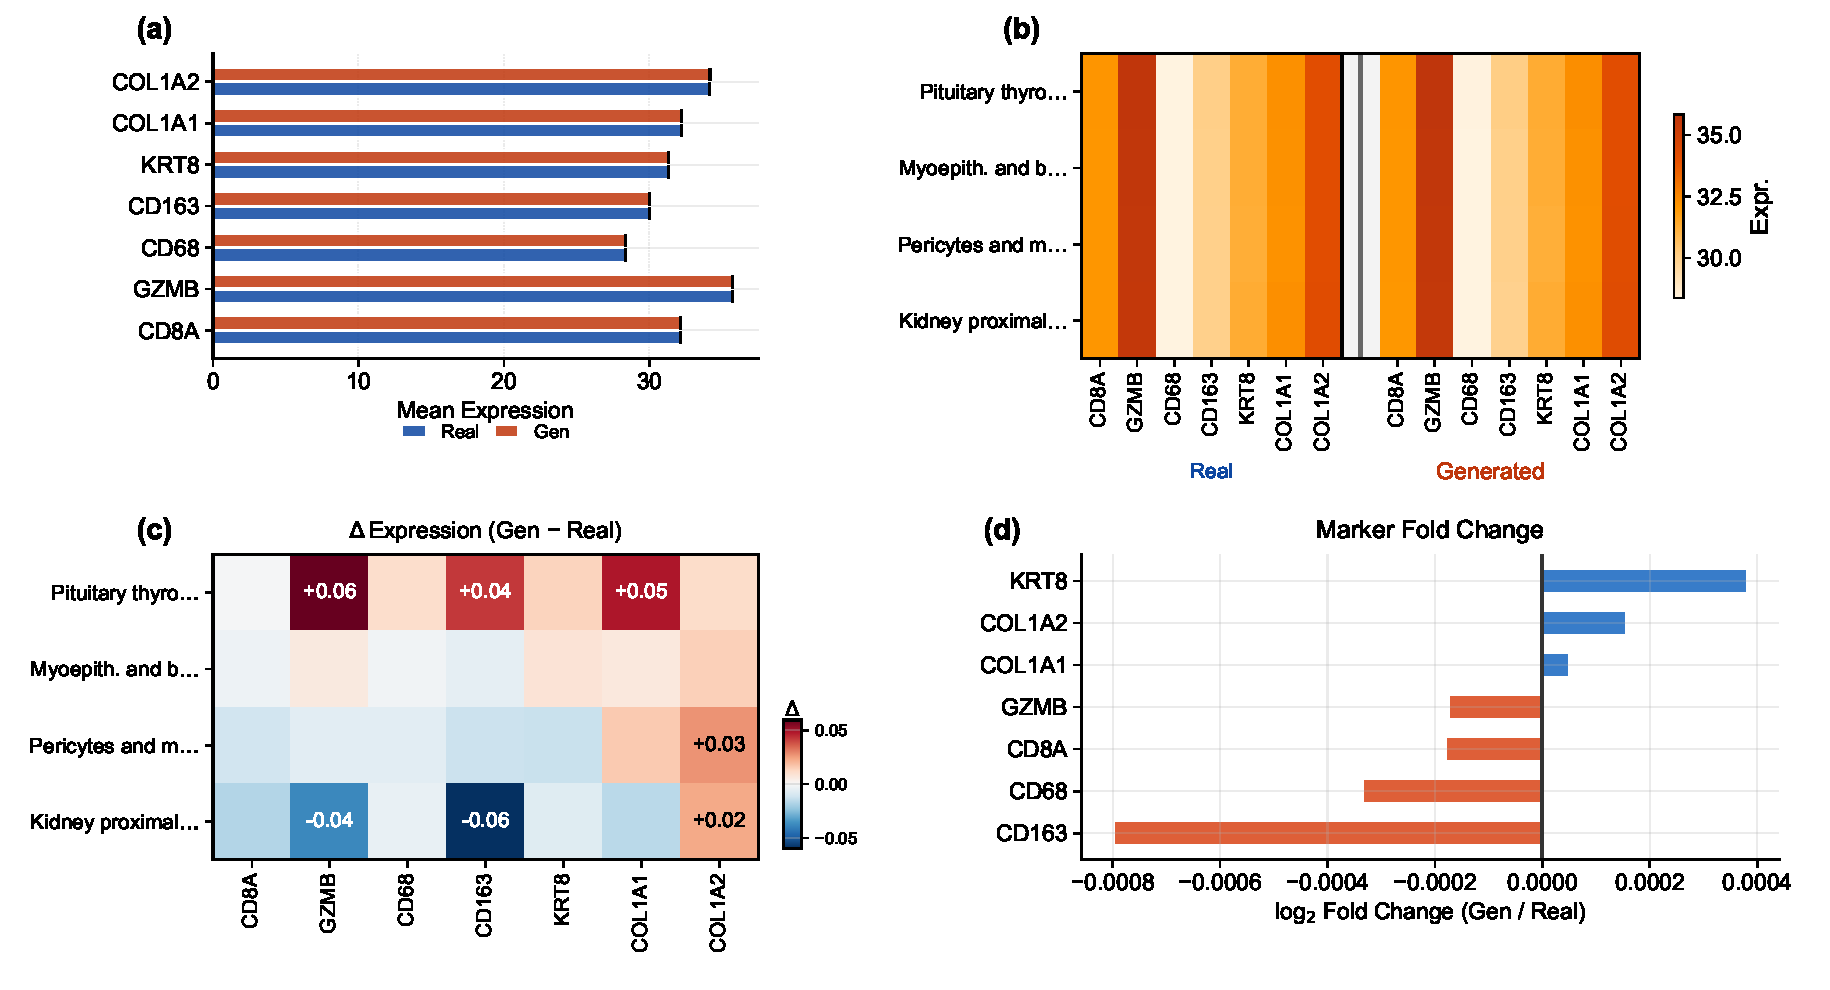
\includegraphics[width=0.95\textwidth]{figures/fig04a_marker_genes.pdf}\par\vspace{-4pt}
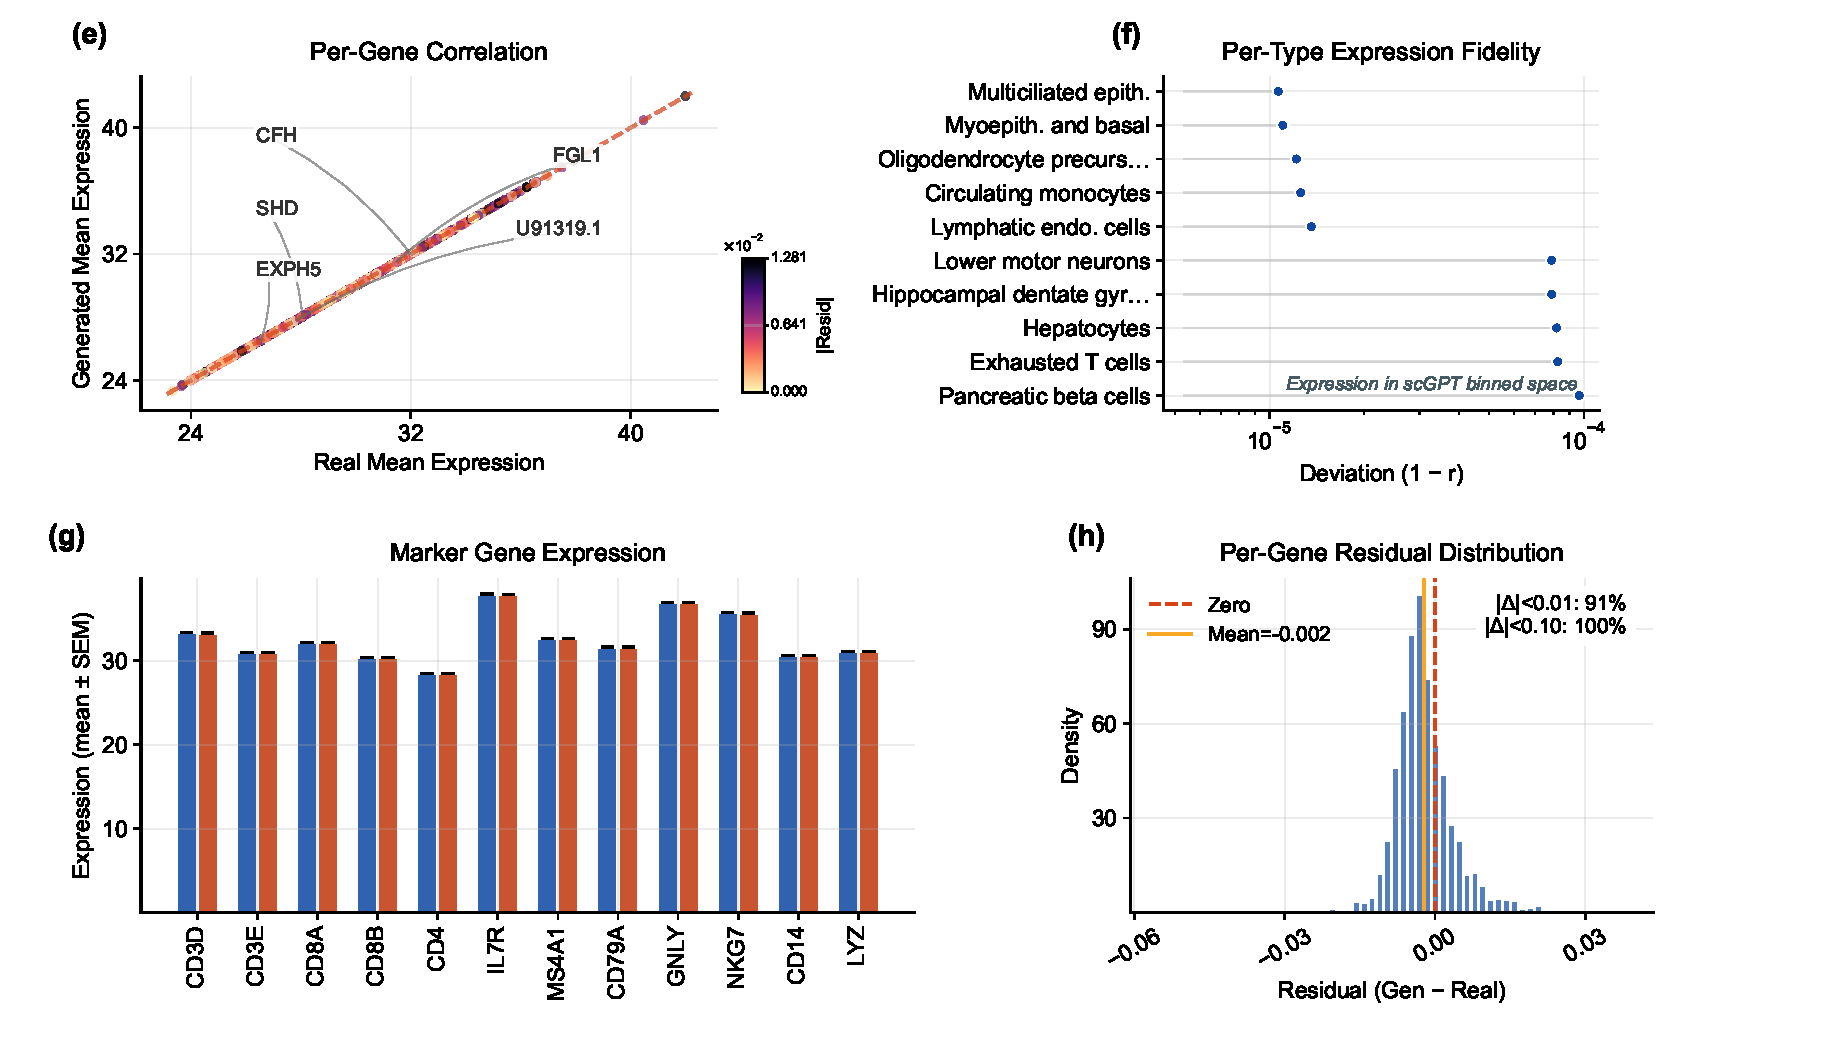
\includegraphics[width=0.95\textwidth]{figures/fig04b_expression_correlation.pdf}
\caption{\textbf{Gene-level fidelity analysis.} \emph{Top row} (marker gene comparison): (\textbf{a})~Paired bar chart of canonical marker gene expression in real vs.\ generated cells. (\textbf{b})~Per-type $\times$ marker dual heatmap. (\textbf{c})~Difference heatmap ($\Delta$ = generated $-$ real). (\textbf{d})~Fold-change waterfall. \emph{Bottom row} (expression correlation): (\textbf{e})~Per-gene mean expression scatter with residual coloring. (\textbf{f})~Per-type deviation from perfect correlation ($1 - r$, log scale). (\textbf{g})~Marker-gene expression comparison with error whiskers. (\textbf{h})~Per-gene residual distribution.\label{fig:gene-fidelity}\label{fig:markers}\label{fig:expr-corr}}
\end{figure}

\begin{figure}[!htbp]
\centering
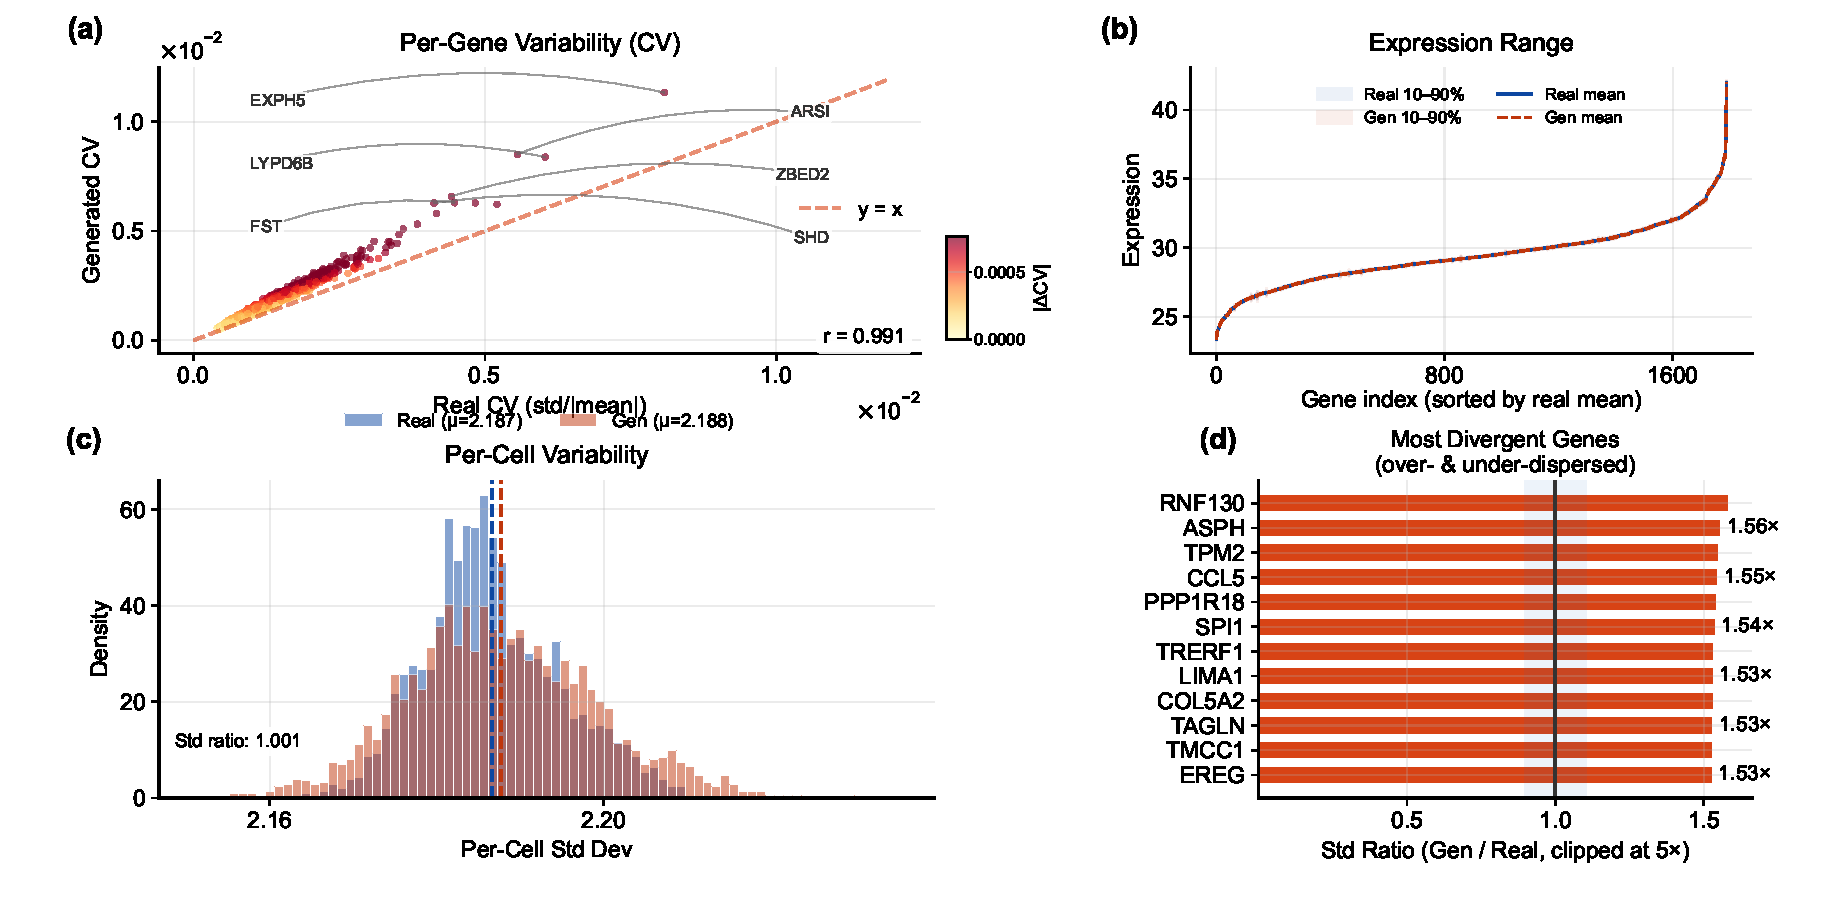
\includegraphics[width=0.95\textwidth]{figures/fig05a_expression_analysis.pdf}\par\vspace{0pt}
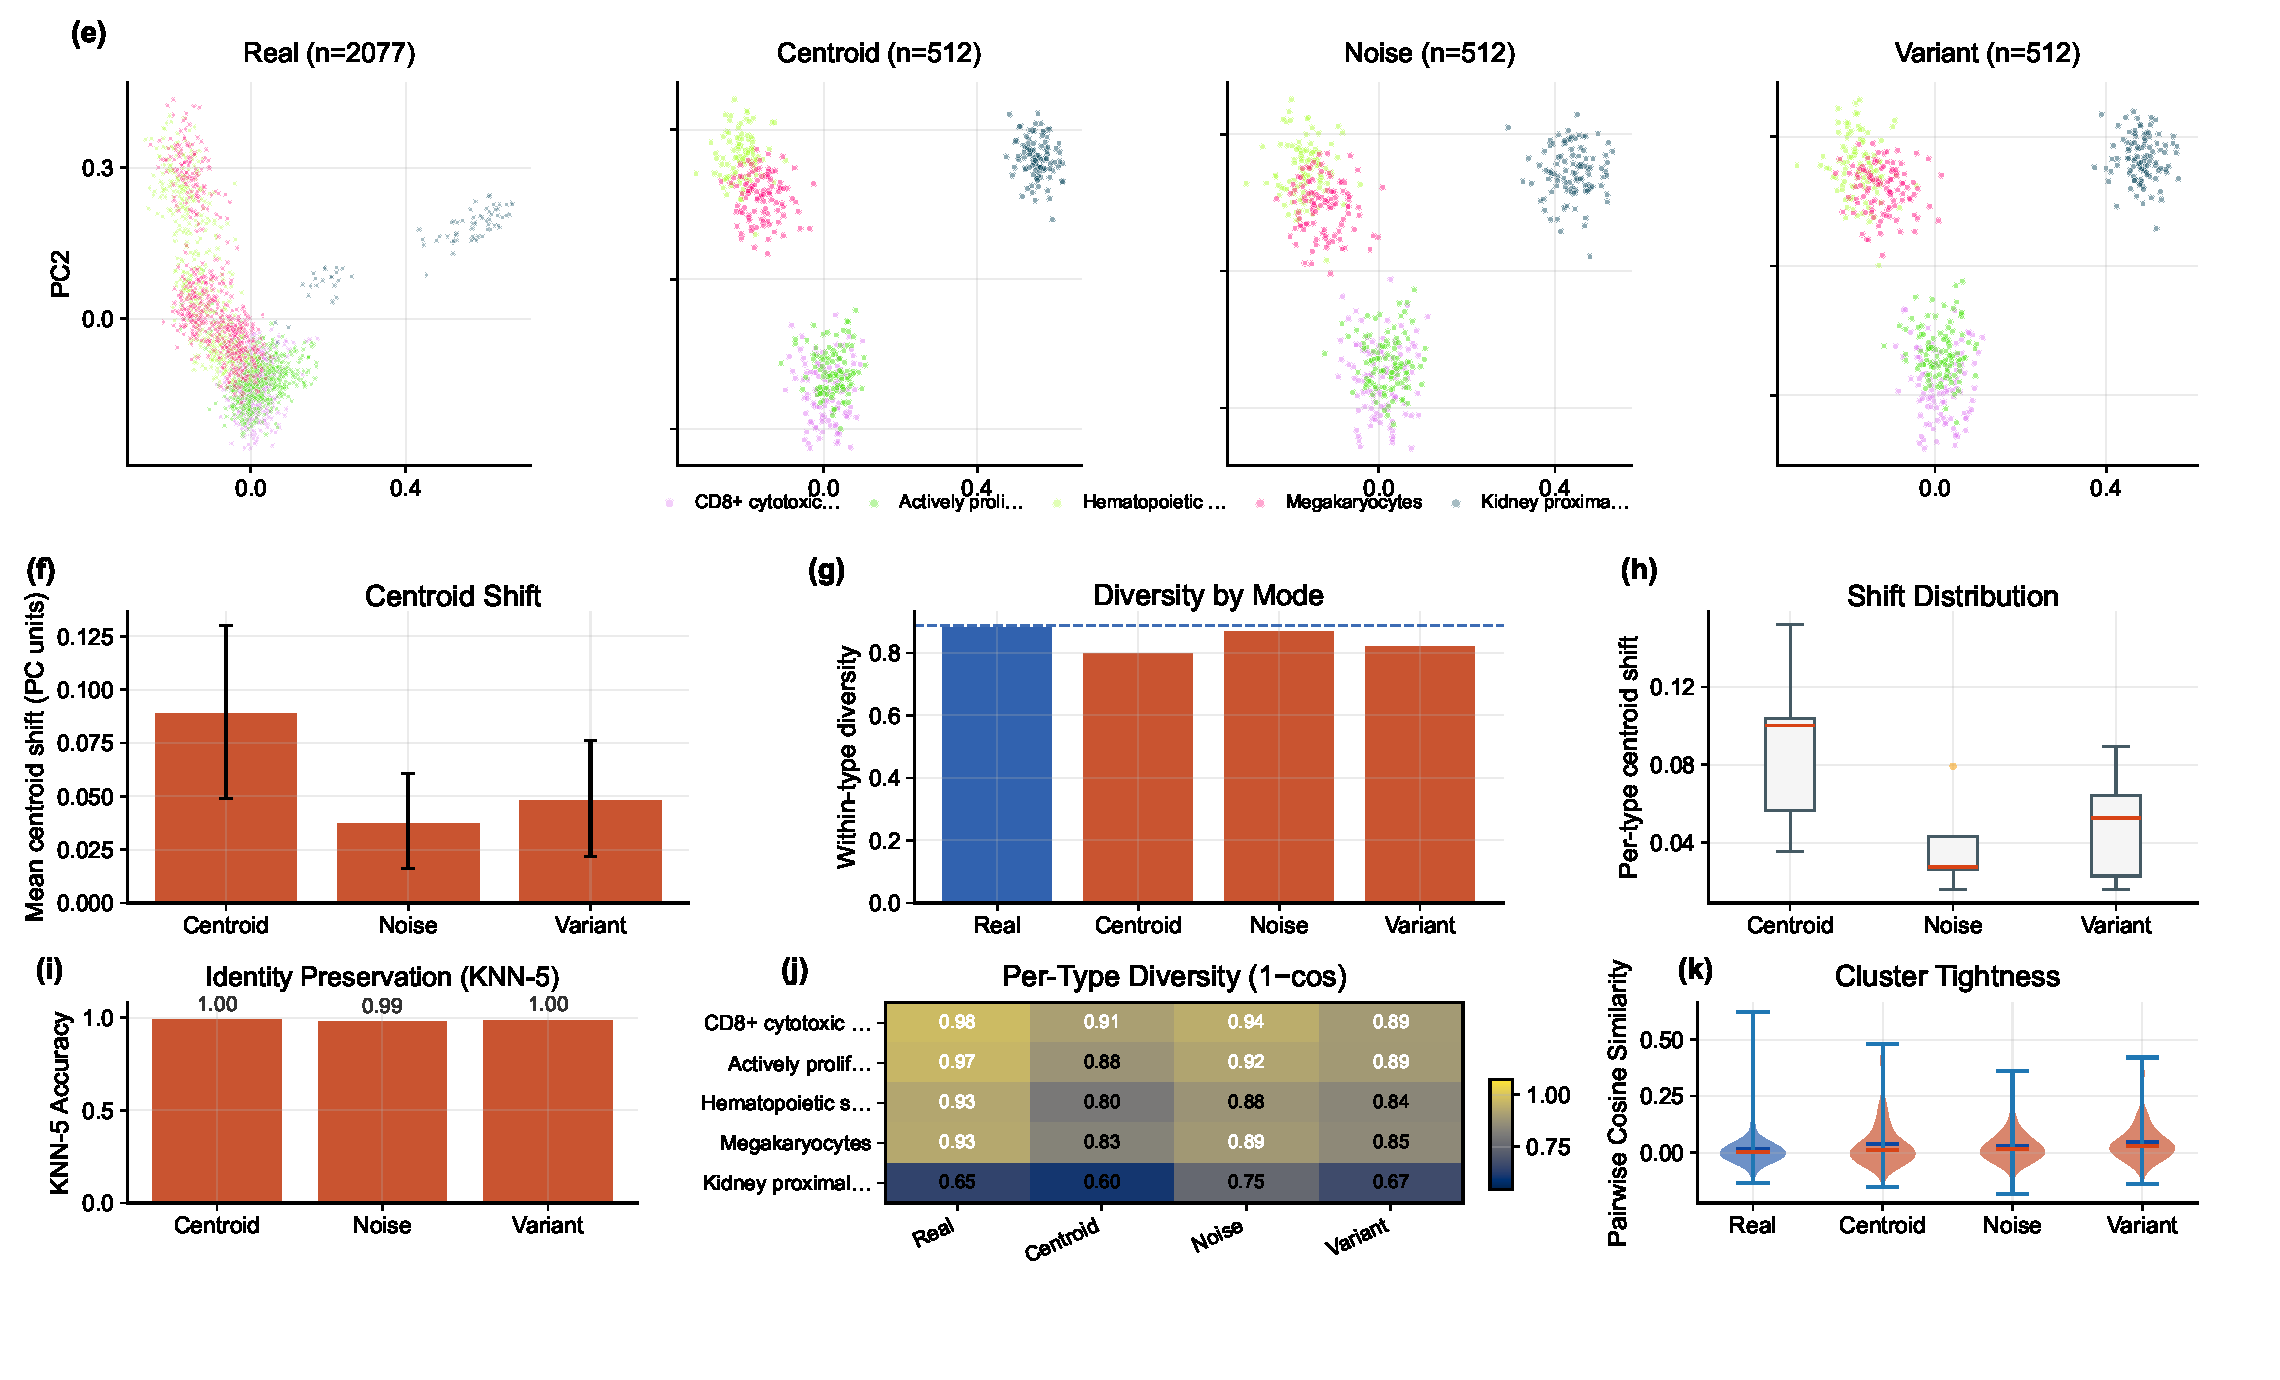
\includegraphics[width=0.95\textwidth]{figures/fig05b_conditioning_landscape.pdf}
\caption{\textbf{Expression distribution analysis and conditioning landscape.} \textbf{(Top)} (\textbf{a})~Per-gene coefficient-of-variation scatter (real vs.\ generated) with abbreviated outlier callouts moved to the panel margin. (\textbf{b})~Expression-range ribbons. (\textbf{c})~Per-cell variability distributions. (\textbf{d})~Top variable genes ranked by standard-deviation ratio. \textbf{(Bottom)} (\textbf{e})~PCA projection of real and generated cells under three conditioning modes (centroid, noisy, variant); the shared cell-type legend is placed beneath the panel set to keep the scatter axes clear. (\textbf{f})~Mean centroid shift per mode. (\textbf{g})~Within-type diversity by mode relative to the real baseline. (\textbf{h})~Per-type centroid shift distributions. (\textbf{i})~KNN-5 identity-preservation accuracy. (\textbf{j})~Per-type diversity heatmap ($1 - \text{mean cosine}$). (\textbf{k})~Pairwise cosine violin plots comparing cluster tightness across modes.\label{fig:expr-analysis}\label{fig:cond-umap}}
\end{figure}

\subsection{Conditioning Landscape and Diversity Trade-Offs}

\noindent After establishing headline fidelity metrics, we next ask how controllable the generator is and how much diversity is sacrificed as guidance increases.

Figure~\ref{fig:cond-umap} shows that CLOP conditions occupy a well-separated landscape in projection space and that generated latent clouds follow this organization, enabling interpretable control over cell-type identity. Together with Figures~\ref{fig:diversity} and~\ref{fig:expr-diversity}, this section therefore serves as the main robustness analysis for whether stronger steering can be achieved without erasing biologically meaningful heterogeneity.

Figure~\ref{fig:diversity} breaks this trade-off into interpretable diagnostics rather than a single scalar summary. Most cell types remain under-dispersed relative to real data, yet nearest-neighbour distances stay above the memorization threshold. Increasing classifier-free guidance monotonically contracts within-type spread, whereas adding conditioning noise partially restores diversity without destroying centroid alignment. The practical outcome is a two-regime operating envelope: stronger guidance improves type fidelity, while Midpoint sampling at CFG = 1.0 best preserves expression-level diversity (Figure~\ref{fig:expr-diversity}) and yields the most balanced gene-level variance profile.

\begin{figure}[!htbp]
\centering
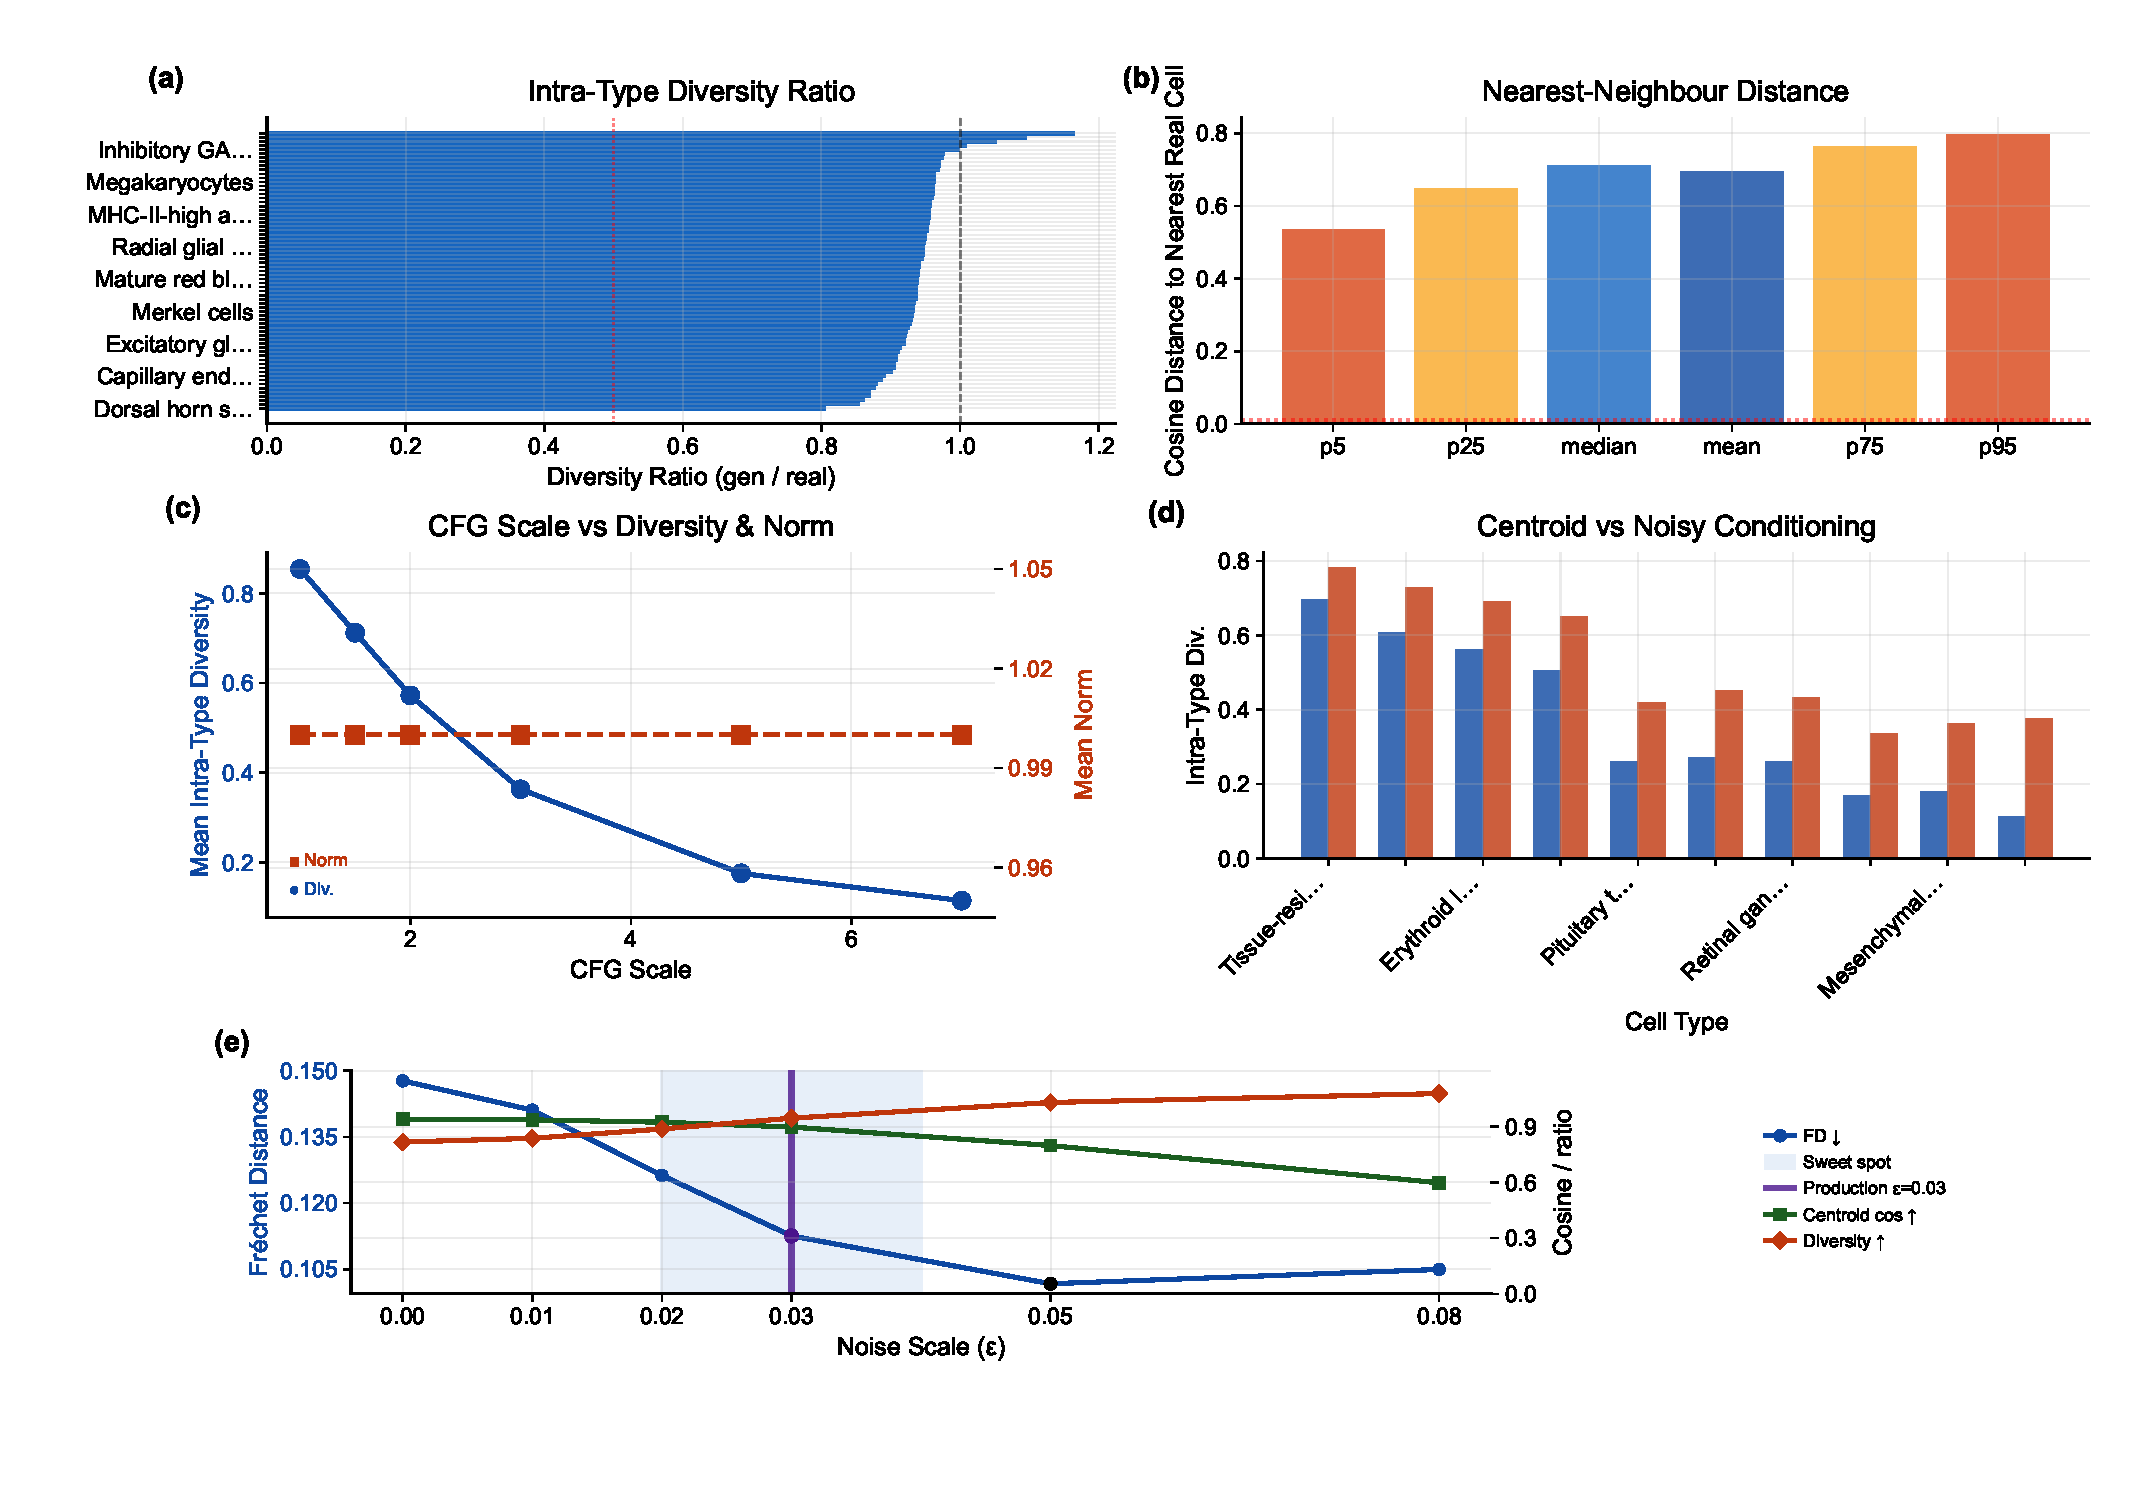
\includegraphics[width=0.95\textwidth]{figures/fig06_diversity_diagnostics.pdf}
\caption{\textbf{Diversity diagnostics and noise-scale trade-off.} (\textbf{a})~Intra-type diversity ratio (generated/real) ranked across cell types; the dashed line marks the ideal ratio of 1.0. (\textbf{b})~Percentiles of the cosine distance from each generated cell to its nearest real-cell neighbour; the dotted line marks the memorization threshold. (\textbf{c})~Classifier-free guidance (CFG) scale versus mean intra-type diversity and mean latent norm. (\textbf{d})~Per-type intra-type diversity under centroid-only versus centroid+noise conditioning. (\textbf{e})~Noise-scale sweep showing Fr\'{e}chet distance, centroid cosine, and diversity ratio as functions of $\varepsilon$; the legend is placed to the right of the panel to keep the plotting area unobstructed, the shaded band marks the sweet-spot region, and the vertical line marks the production configuration ($\varepsilon = 0.03$).\label{fig:diversity-suite}\label{fig:diversity}\label{fig:noise-tradeoff}}
\end{figure}

\begin{figure}[!htbp]
\centering
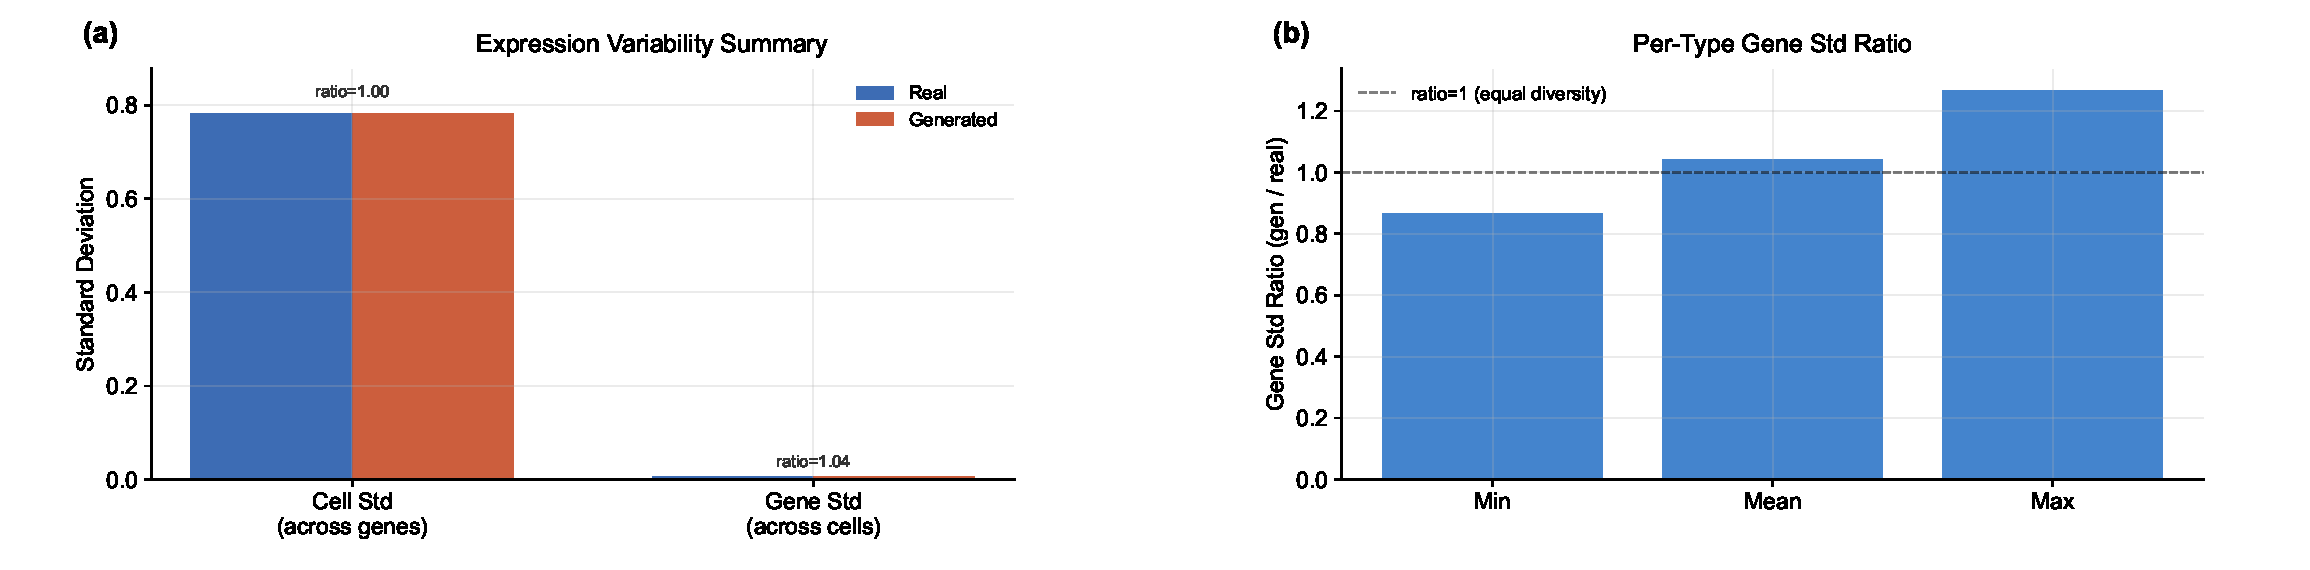
\includegraphics[width=0.95\textwidth]{figures/fig07a_expression_diversity.pdf}\par\vspace{0pt}
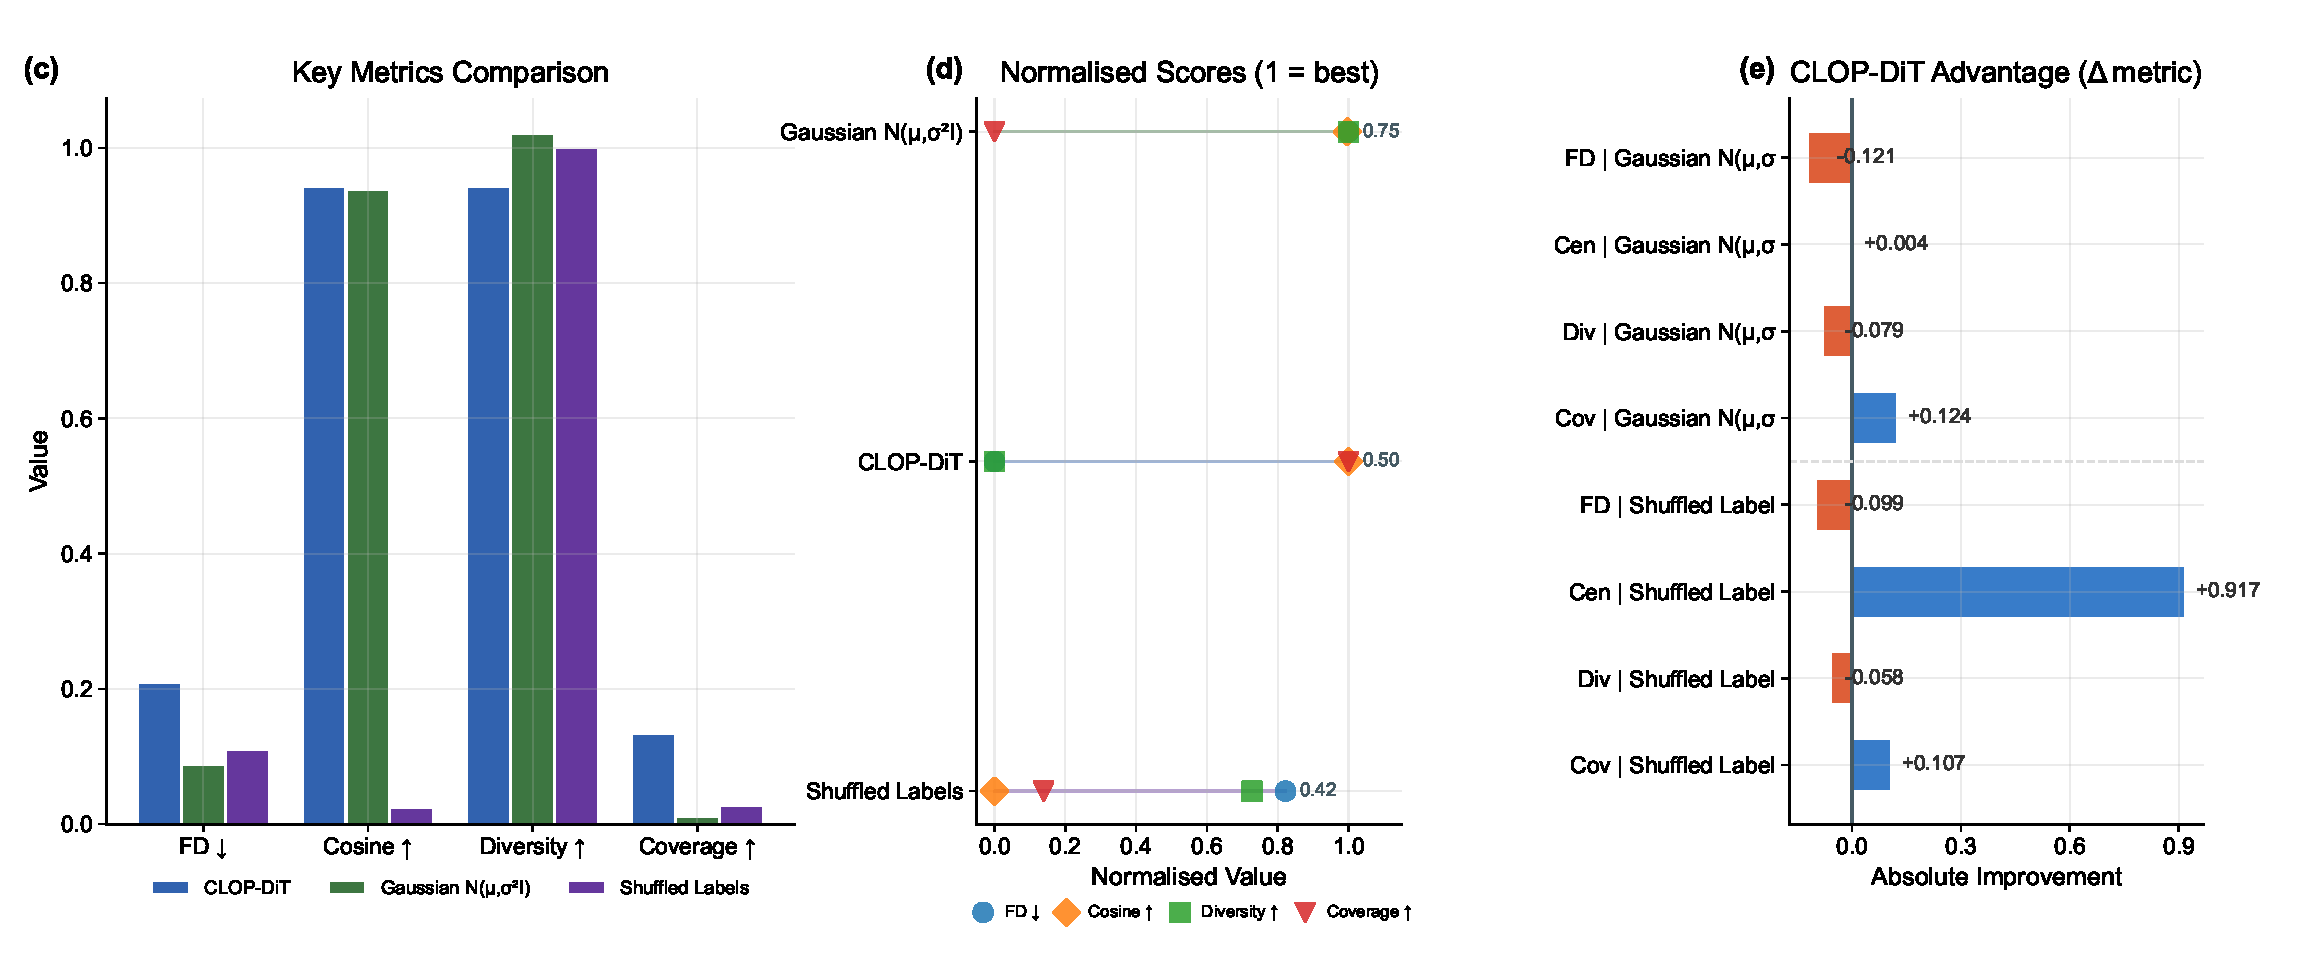
\includegraphics[width=0.95\textwidth]{figures/fig07b_baseline_comparison.pdf}\par\vspace{0pt}
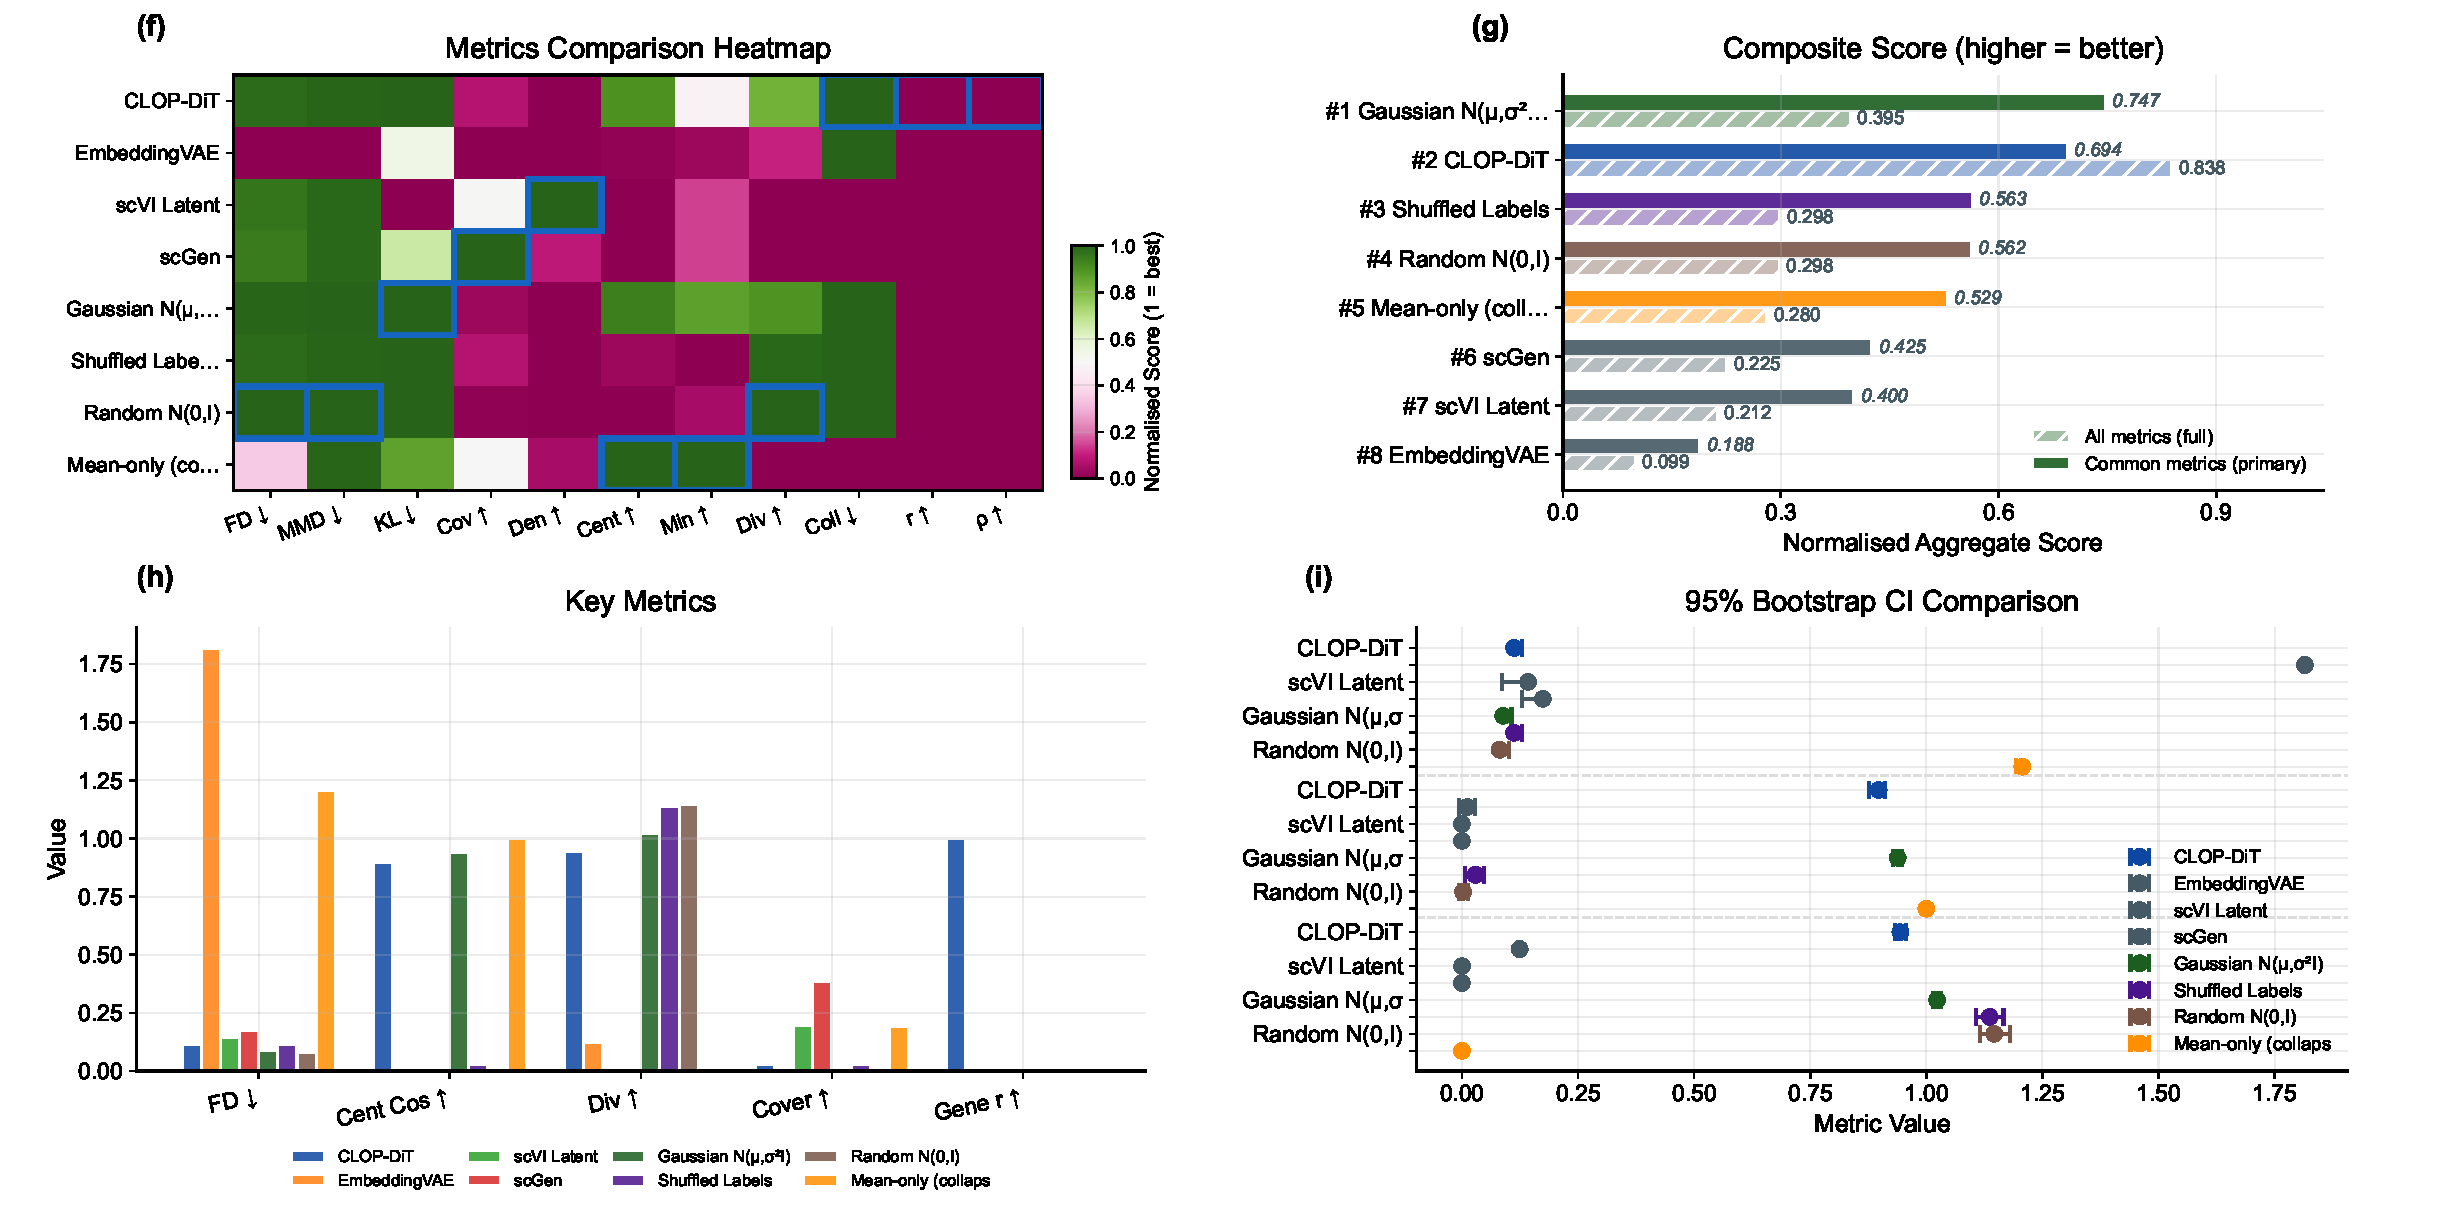
\includegraphics[width=0.95\textwidth]{figures/fig07c_benchmark.pdf}
\caption{\textbf{Expression-level diversity, baseline comparison, and composite benchmark.} \textbf{(Top)} (\textbf{a})~Gene-expression variability summary (real vs.\ generated). (\textbf{b})~Per-type gene standard-deviation ratio. \textbf{(Middle)} (\textbf{c})~Head-to-head grouped-bar analysis across four evaluation metrics. (\textbf{d})~Ranked normalised scores per method. (\textbf{e})~Absolute metric delta of CLOP-DiT relative to each baseline. \textbf{(Bottom)} (\textbf{f})~Normalized metrics heatmap (methods $\times$ metrics). (\textbf{g})~Composite score (solid = common-metrics-only; hatched = full). \textbf{Warning: the full composite is structurally biased}; the common-metrics-only bars are the fair comparison. (\textbf{h})~Grouped comparison of four interpretable metrics. (\textbf{i})~95\% bootstrap confidence intervals.\label{fig:expr-diversity}\label{fig:baselines}\label{fig:benchmark}}
\end{figure}

\subsection{Baseline Comparison and Composite Benchmark}

\noindent We benchmark CLOP-DiT against both simple parametric controls (Gaussian per-type sampling, shuffled-label controls, mean-collapse baselines) and learned generative models (scVI Latent, scGen, EmbeddingVAE).

CLOP-DiT is compared against unconditional generation (CFG = 0), Gaussian sampling from per-type statistics, shuffled-label and mean-collapse controls, EmbeddingVAE, scVI Latent~\citep{ref-scvi}, and a conditional scGen baseline~\citep{ref-scgen} implemented as conditional scVI with cell-type covariates. Figure~\ref{fig:baselines} reveals a consistent pattern: CLOP-DiT is strongest on conditioning-sensitive and downstream-relevant metrics, especially steering and classifier transfer, whereas unconditional or weakly conditioned baselines can score better on FD-like objectives because those metrics reward global moment matching even when cell-type steering is absent.

Figure~\ref{fig:benchmark} aggregates these results into a composite score across eight methods. \textbf{On the nine distributional metrics shared by all methods---the primary fair comparison---the Gaussian baseline (0.747) slightly exceeds CLOP-DiT (0.694)}, showing that simple mean-matching approaches remain competitive when evaluation ignores condition-sensitive biology. The scGen baseline (common-metrics composite 0.425) achieves the best \emph{coverage} among the learned baselines (0.384 vs.\ 0.028 for CLOP-DiT), reflecting the flexibility of its label-conditioned VAE latent space. When the eight downstream biology metrics reported only by CLOP-DiT are included, the full composite rises to 0.838 versus 0.395 for Gaussian and 0.225 for scGen; however, this full score is structurally biased in favor of CLOP-DiT and \textbf{should not be used for method ranking}. We therefore treat the common-metrics-only composite as the main benchmark and the full composite as a supplementary capability summary.

\subsection{Downstream Biological Validation}

Beyond distributional metrics, we evaluate whether generated cells are usable in standard single-cell analysis workflows. These analyses are implemented from matched real/generated AnnData objects with shared preprocessing and use Scanpy~\citep{ref-scanpy} for the single-cell workflow, ensuring that any downstream advantage is not caused by mismatched feature engineering. Two downstream tasks are assessed on real and generated cells jointly:

\textbf{Clustering, mixing, and classifier alignment} (Figure~\ref{fig:downstream-pq}): We construct matched AnnData objects from real and generated expression matrices, select 2,000 shared highly variable genes, perform PCA and Leiden~\citep{ref-leiden} clustering on the combined dataset, and compute the Adjusted Rand Index (ARI), Normalized Mutual Information (NMI), cluster purity, and per-type KNN mixing scores~\citep{ref-integration-benchmark}. High mixing scores indicate that generated cells partially co-localize with real cells of the same type in the joint embedding, though the discriminator AUC of 0.656 confirms that real and generated populations remain distinguishable. A logistic regression classifier is trained on real PCA embeddings to predict cell type, then evaluated on generated embeddings to measure transfer accuracy and macro-F1. The enhanced classifier panel reports a per-type precision/recall/F1 heatmap in addition to the confusion matrix and discriminator ROC, demonstrating that downstream performance exhibits strong heterogeneity across cell types. The real-vs.-generated discriminator AUC (0.656) indicates partial but non-trivial separability, so downstream usability remains qualified rather than near-indistinguishable transfer.

\textbf{DE concordance} (Figure~\ref{fig:downstream-r}): Wilcoxon rank-sum differential expression analysis~\citep{ref-wilcoxon} is performed on three biologically meaningful contrasts (CD8 vs.\ CD4 T cells, resident macrophage vs.\ monocyte, epithelial tumor vs.\ fibroblast). We compare log-fold changes between real and generated data via Pearson and Spearman correlations, Jaccard overlap of the top-50 DE genes, and sign-agreement fractions. The enhanced DE figure weights each gene by effect size and colors it by adjusted significance, which separates minor noisy disagreements from the biologically important genes that dominate each contrast.

\begin{figure}[!htbp]
\centering
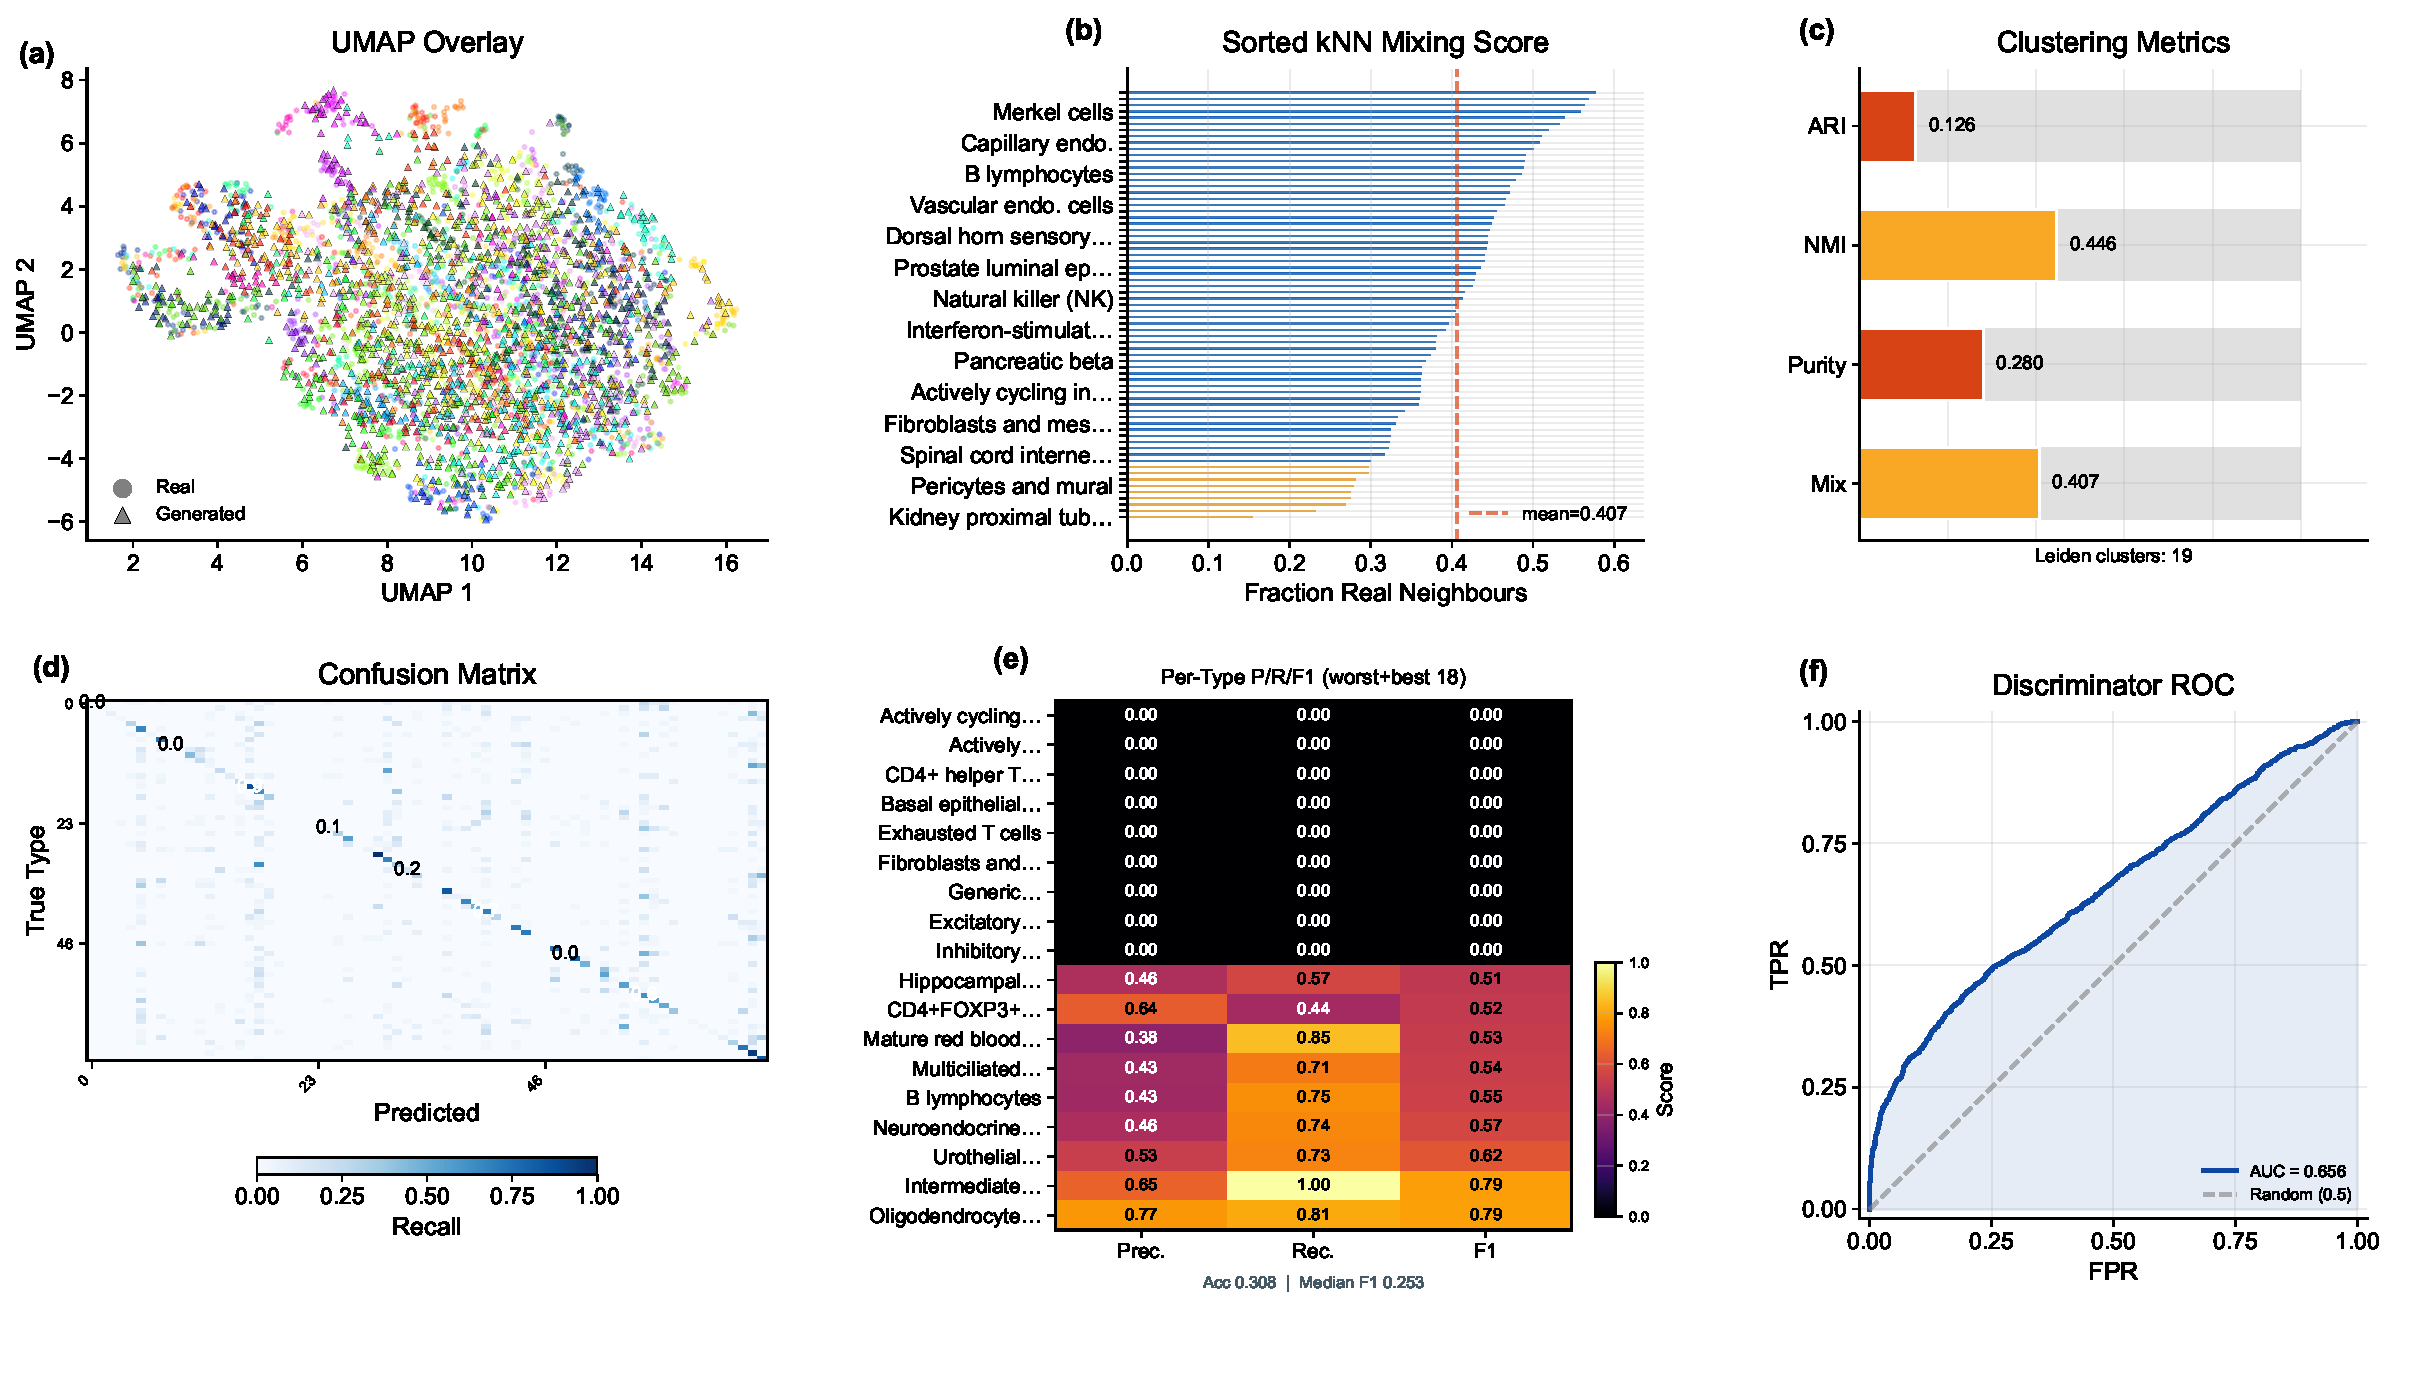
\includegraphics[width=0.95\textwidth]{figures/fig08a_downstream_validation.pdf}\par\vspace{2pt}
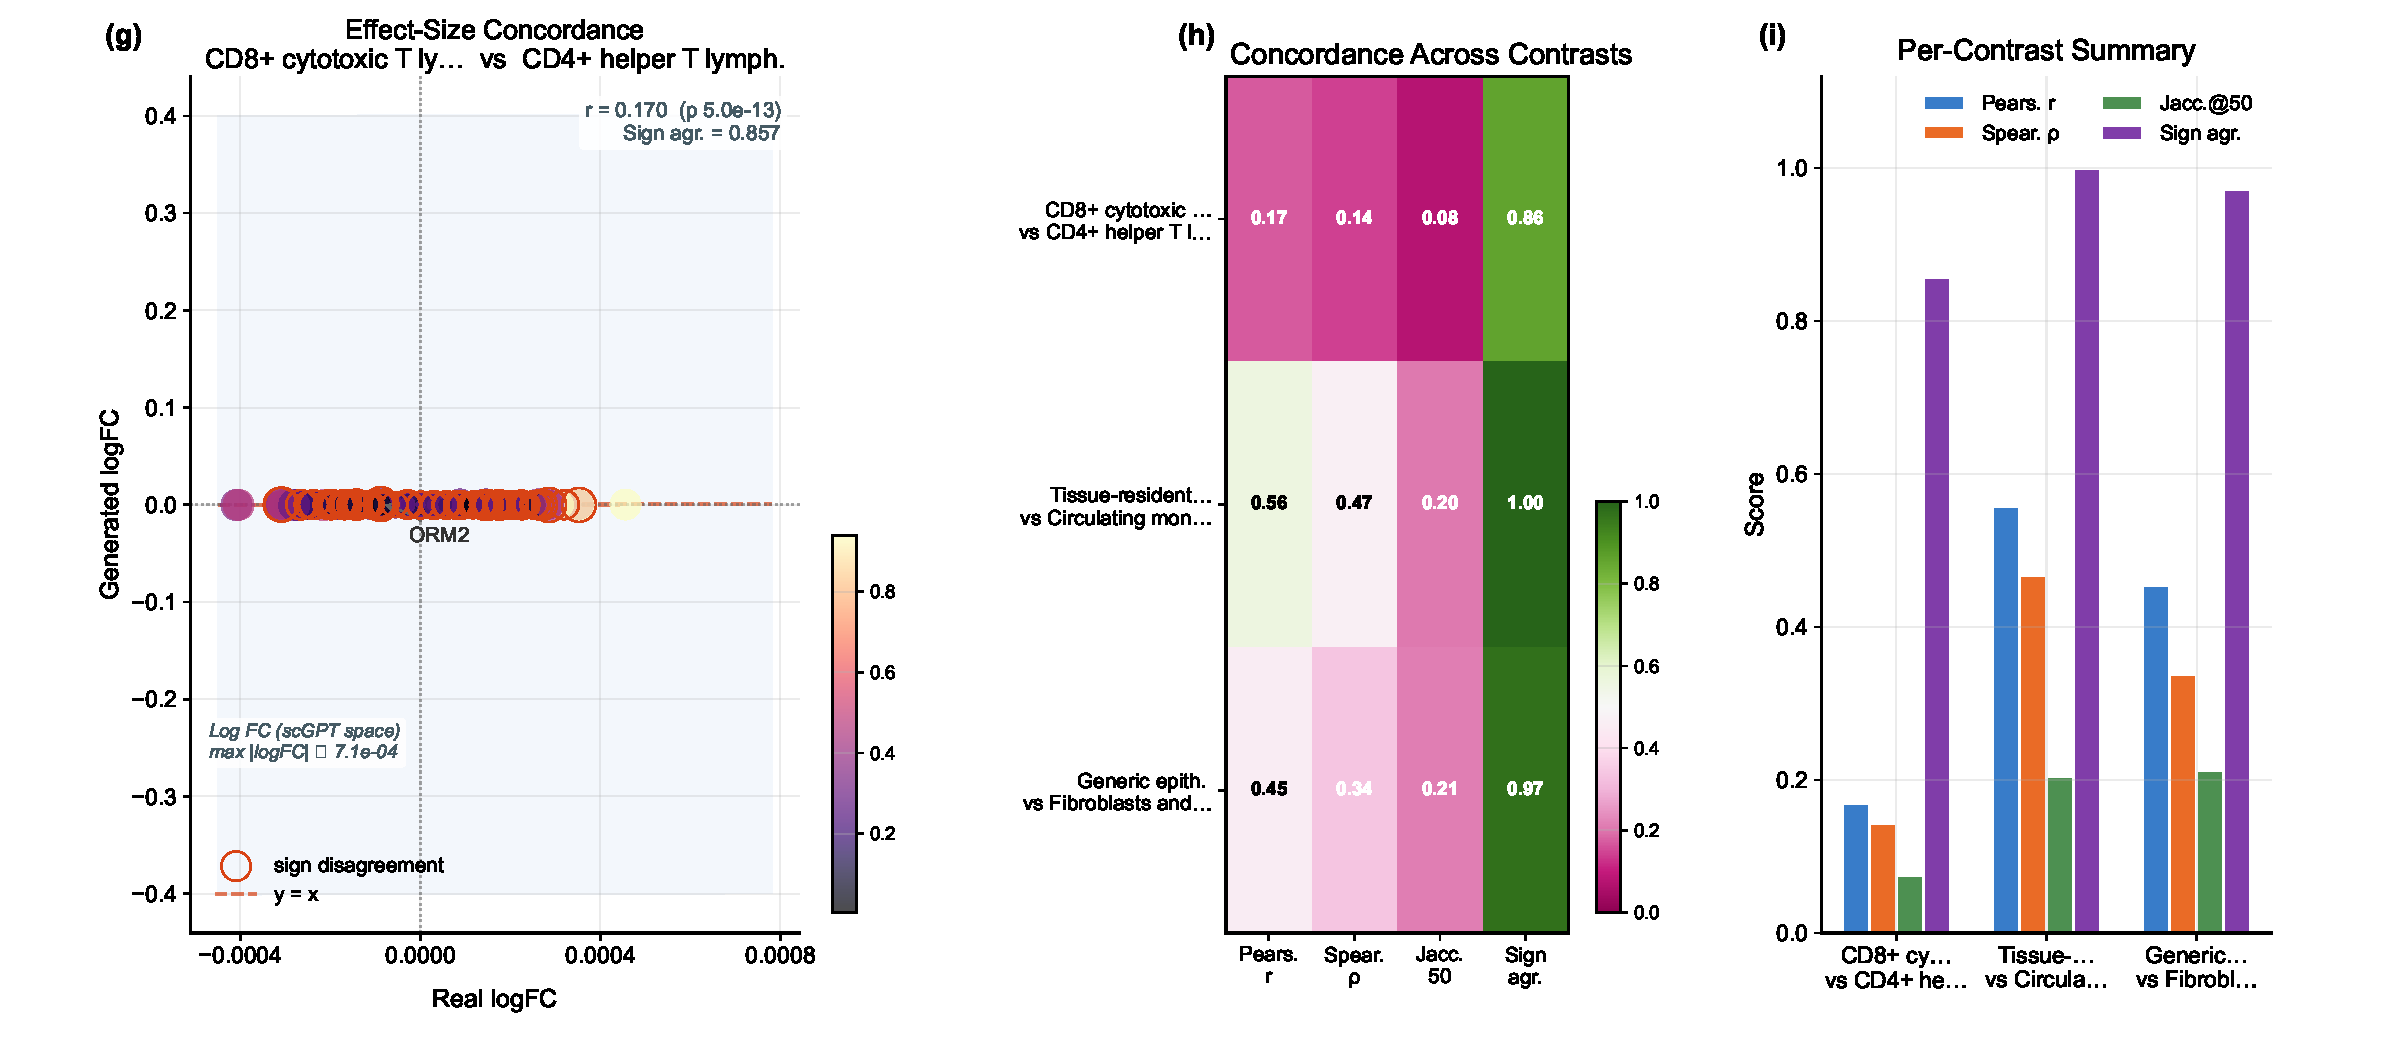
\includegraphics[width=0.95\textwidth]{figures/fig08b_de_concordance.pdf}
\caption{\textbf{Downstream validation.} \textbf{(Top)} (\textbf{a})~Leiden clustering on combined real + generated data with UMAP overlay, (\textbf{b})~sorted per-type KNN mixing profile, and (\textbf{c})~compact cluster-alignment gauges (ARI, NMI, cluster purity, mean KNN mixing). (\textbf{d})~Cell-type classification confusion matrix, (\textbf{e})~precision/recall/F1 heatmap, and (\textbf{f})~real-vs.-generated discriminator ROC curve. \textbf{(Bottom)} (\textbf{g})~Effect-size-weighted logFC scatter for the leading contrast; sign-disagreement genes are outlined. (\textbf{h})~Concordance heatmap (Pearson~$r$, Spearman~$\rho$, Jaccard@50, sign agreement) across three contrasts. (\textbf{i})~Per-contrast grouped-bar summary.\label{fig:downstream-pq}\label{fig:downstream-r}}
\end{figure}

Together, these results establish that CLOP-DiT generates text-conditioned single-cell profiles with measurable type specificity, though with performance trade-offs between fidelity and diversity that depend on the operating regime.

\subsection{In-Distribution Expression-Level Validation}\label{sec:cross-dataset}

To assess biological fidelity across tissue contexts, we performed expression-level validation on five datasets (Table~\ref{tab:s4_biovalidation}) spanning lung adenocarcinoma (GSE123902), basal cell carcinoma (GSE123813), liver T-cell hepatocellular carcinoma (GSE98638), gastric cancer (GSE183904), and acute lymphoblastic leukemia in bone marrow (GSE132509). Four of these five datasets (GSE123902, GSE123813, GSE98638, GSE132509) are from the training split; only GSE183904 is among the 8 held-out validation studies (Table~S2). This analysis therefore primarily evaluates in-distribution gene-level reconstruction fidelity rather than out-of-distribution generalization. For each dataset, cells were generated conditioned on the dataset-specific text descriptions and compared with real (scGPT-reconstructed) expression profiles; because both the generated and reference expressions are decoded by the same frozen scGPT decoder, the resulting correlations measure decoder-reconstructed fidelity rather than agreement with raw sequencing counts. Per-gene mean expression, gene-level variance, and Fr\'{e}chet distance in both gene space and embedding space were computed for each dataset independently (Table~\ref{tab:cross-dataset}).

\begin{table}[!htbp]
\caption{Cross-dataset biological validation (decoder-reconstructed fidelity). Per-gene mean expression Pearson correlation ($r$) and coefficient of determination ($R^2$), gene variance Pearson correlation ($r_\text{var}$), and Fr\'{e}chet distance in PCA-50 gene space (FD\textsubscript{gene}) and scGPT embedding space (FD\textsubscript{embed}) for real and generated cells. Both ``real'' and generated expression profiles are decoded by the same frozen scGPT decoder; correlations therefore measure decoder-reconstruction consistency rather than agreement with raw sequencing counts. Split indicates whether the dataset was used for training (Train) or held-out validation (Val). All five datasets achieve gene\_mean $r > 0.999$.\label{tab:cross-dataset}}
\centering
\small
\begin{tabular}{lccccccc}
\toprule
\textbf{Dataset (GEO)} & \textbf{Tissue} & \textbf{Split} & \textbf{$r_\text{mean}$} & \textbf{$R^2$} & \textbf{$r_\text{var}$} & \textbf{FD\textsubscript{gene}} & \textbf{FD\textsubscript{embed}} \\
\midrule
GSE123902 & Lung     & Train & 0.9995 & 0.9990 & $+$0.011  & $3.07 \times 10^{-5}$ & 73.9 \\
GSE123813 & Skin (BCC)  & Train & 0.9997 & 0.9995 & $-$0.019  & $5.25 \times 10^{-6}$ & 72.7 \\
GSE98638  & Liver    & Train & 0.9995 & 0.9989 & $-$0.003  & $2.04 \times 10^{-5}$ & 155.4 \\
GSE183904 & Gastric  & Val & 0.9997 & 0.9994 & $+$0.013  & $1.30 \times 10^{-5}$ & 62.1 \\
GSE132509 & Blood (ALL)  & Train & 0.9993 & 0.9985 & $-$0.007  & $8.87 \times 10^{-6}$ & 69.1 \\
\bottomrule
\end{tabular}
\end{table}

Across all five datasets, per-gene mean expression Pearson correlation exceeds 0.999 and $R^2$ exceeds 0.998. Because both reference and generated profiles pass through the same frozen scGPT decoder, these correlations reflect decoder-reconstructed fidelity rather than absolute biological accuracy against raw counts. However, per-gene variance correlation ($r_\text{var}$) is near zero across all datasets (range: $-0.019$ to $+0.013$), indicating that the model reproduces mean expression accurately but does not preserve gene-level variability---consistent with the flow-matching mean-regression bias. Embedding-space FD (62.1--155.4) is substantially higher than gene-space FD ($<10^{-4}$), reflecting the many-to-one decoder mapping.

\subsection{CLOP Ablation Study}\label{sec:ablation}

To validate the contribution of individual CLOP components, we conducted 15 ablation experiments, removing or modifying one component at a time while holding all other settings constant. Table~\ref{tab:ablation} summarizes the six most informative ablations.

\begin{table}[!htbp]
\caption{CLOP ablation study (\textbf{ablation baseline only}; not the final production model). Validation prototype accuracy (top-1) for the ablation baseline configuration (all features enabled) and representative ablations. $\Delta$~denotes the change from baseline in percentage points. These results characterize the CLOP alignment stage in isolation and do not directly predict downstream DiT generation quality; the final production model uses different regularization settings.\label{tab:ablation}}
\centering
\small
\begin{tabular}{llcc}
\toprule
\textbf{Ablation} & \textbf{Category} & \textbf{Val Proto Acc (\%)} & \textbf{$\Delta$ (pp)} \\
\midrule
$-$cohesion        & regularization & 86.41 & $+$10.24 \\
$-$cell noise      & regularization & 86.23 & $+$10.07 \\
$-$dropout (lighter) & regularization & 77.32 & $+$1.15 \\
Baseline           & reference      & 76.17 & --- \\
Fixed temperature   & optimization   & 71.55 & $-$4.61 \\
High variant prob   & regularization & 70.14 & $-$6.03 \\
\bottomrule
\end{tabular}
\end{table}

The two most impactful ablations are cohesion regularization removal ($+$10.24~pp) and cell noise augmentation removal ($+$10.07~pp), both of which improve prototype accuracy. This counterintuitive result has the following mechanistic explanation: both cohesion loss and cell noise augmentation act as within-group tightening forces that penalize intra-cluster variance. In a contrastive learning regime where the primary bottleneck is inter-group separation (raw pairwise cosine 0.994), these tightening forces compete with the alignment gradient rather than complementing it. In effect, the network spends representational capacity enforcing tight within-group clusters before inter-group margins have been established, diverting training signal from the discrimination task. Removing these terms allows the optimizer to focus entirely on inter-group separation, which is the binding constraint at this scale. This interpretation is consistent with recent analyses of regularization--discrimination trade-offs in contrastive learning~\citep{ref-siglip}. Architecture ablations (projection dimension 256 vs.\ 512 vs.\ 768) have minimal impact (within $\pm$0.3~pp), indicating that the CLOP aligner is not sensitive to projection dimension in this range. Fixed temperature ($-$4.61~pp) and high variant probability ($-$6.03~pp) degrade performance substantially relative to the ablation baseline (which used a learnable temperature). \textbf{Clarification:} The ablation baseline used a learnable $\tau$, whereas the final production model uses fixed $\tau = 14.0$ in combination with a stratified validation split (Section~\ref{sec:dataset}). The production configuration was selected based on the full-pipeline generation quality assessment, not solely on CLOP prototype accuracy; the ablation table characterizes the CLOP alignment stage in isolation and does not directly predict downstream DiT generation performance.

\subsection{Rare Cell Augmentation}\label{sec:rare-cell}

As a proof-of-concept, we evaluated whether generated cells can improve classifier performance on an underrepresented type (``Cycling cells'', $<$5\% prevalence). Augmentation at 1--10$\times$ ratios did not improve Cycling-cell F1 (baseline 0.828 $\to$ 0.741--0.786 after augmentation), though overall macro F1 remained stable (0.947--0.964), indicating that synthetic profiles are realistic enough to avoid catastrophic interference but lack the within-type heterogeneity needed for net positive augmentation.

\subsection{Conditioning Field Ablation and Swap-Label Permutation Test}\label{sec:cond-ablation}

To assess whether the conditioning signal causally steers generation---rather than the model recapitulating training-set structure regardless of prompt content---we performed two targeted experiments.

\textbf{Conditioning field ablation.} We generated 50 cells per type across all 69 cell types (3,450 cells per variant) under five prompt variants: (i)~\emph{full}: the complete structured prompt; (ii)~\emph{no-markers}: marker gene fields removed; (iii)~\emph{shuffled-markers}: marker gene lists randomly permuted across types; (iv)~\emph{metadata-only}: only organism, tissue, and disease fields retained; (v)~\emph{external-markers}: canonical markers from PanglaoDB/CellMarker~2.0 substituted for the training markers (evaluated on 15 well-characterized types). Table~\ref{tab:cond-ablation} reports KNN accuracy, steering accuracy, and centroid cosine similarity for each variant.

\begin{table}[!htbp]
\centering
\caption{Conditioning field ablation results (CFG = 2.0, Euler solver, 10 steps, 50 cells per type). KNN accuracy assessed against real-cell references using the ablation-specific generation cache (freshly encoded prompt variants), which differs from the primary evaluation cache in Table~\ref{tab:core-results} (cached training-time CLOP conditions, 200 cells per type); the lower KNN values reflect the use of re-encoded prompt embeddings rather than the optimized training-time conditions. Steering measured as cosine alignment to the target type centroid; centroid cosine is the mean cosine similarity between generated and real centroids. The external-markers variant was evaluated on a 15-type subset with consensus markers from PanglaoDB and CellMarker~2.0.\label{tab:cond-ablation}}
\begin{tabular}{lrrr}
\toprule
Prompt variant & KNN (\%) & Steering (\%) & Centroid cos. \\
\midrule
Full (all fields) & 2.87 & 99.8 & 0.050 \\
No markers & 2.26 & 98.0 & 0.035 \\
Shuffled markers & 2.81 & 97.9 & 0.035 \\
Metadata only & 1.51 & 62.4 & 0.025 \\
External markers (15 types) & 17.07 & --- & 0.702$^*$ \\
\bottomrule
\multicolumn{4}{l}{\footnotesize $^*$Cosine similarity between external-marker and full-prompt centroids.}
\end{tabular}
\end{table}

The results indicate that semantic content contributes to the conditioning signal beyond prompt length alone: removing only the marker field reduces centroid cosine from 0.050 to 0.035 (30\% relative drop), while retaining only metadata fields collapses steering from 99.8\% to 62.4\%. Substituting external markers from independent databases yields a high cosine similarity to the full-prompt variant (0.702), indicating that the model responds to marker-gene semantics rather than memorized training prompts.

\textbf{Swap-label permutation test.} To test whether generation follows the conditioning signal causally, we generated 15 cell-type pairs where the prompt for type $A$ was used to condition generation but evaluation was performed against both type $A$ (matched) and type $B$ (mismatched) real-cell centroids. In 9 of 15 pairs, the generation conditioned on the matched prompt was closer to the real centroid of type $A$ than the mismatched generation (matched cosine similarity 0.032 vs.\ mismatched 0.016, gap = 0.016). Critically, in all 15 of 15 pairs the mislabeled generation---conditioned on text$_B$ but evaluated against real cluster $A$---followed the conditioning signal (text$_B$) rather than the evaluation label, confirming that the model generates latents based on prompt semantics rather than memorized label identity. The sub-unity matched-wins rate (9/15) reflects the small magnitude of centroid cosine differences in the tightly packed scGPT embedding space rather than a failure of causal conditioning. While this test does not fully exclude encoder-level leakage, it provides causal evidence that the conditioning channel is functional and semantically interpretable.

\section{Discussion}\label{sec:discussion}

CLOP-DiT demonstrates that structured-text conditioning can drive non-trivial conditional generation in tightly-packed biological embedding spaces. The framework's primary contribution is architectural: a modular pipeline where contrastive alignment, conditional flow matching, and frozen decoding are independently trainable and replaceable. We discuss the main computational findings, open problems, and design implications below.

\textbf{Second-order structure preservation.} The central open problem is preserving within-class variance and covariance. Despite augmenting flow matching with per-group variance matching ($\lambda_\text{var}=0.10$) and sliced covariance regularization ($\lambda_\text{cov}=0.05$), generated distributions remain under-dispersed. In-distribution variance trends are partially recovered ($r = 0.98$, Figure~\ref{fig:variance-deepdive}), but cross-dataset variance correlation falls near zero and gene--gene correlations are poorly preserved. This is a fundamental challenge in conditional flow matching: the optimal-transport interpolant encourages mean-seeking trajectories, and group-level regularizers only partially counteract this tendency. Future work on trajectory-level diversity objectives or diffusion-based alternatives may offer better variance preservation.

\begin{figure}[!htbp]
\centering
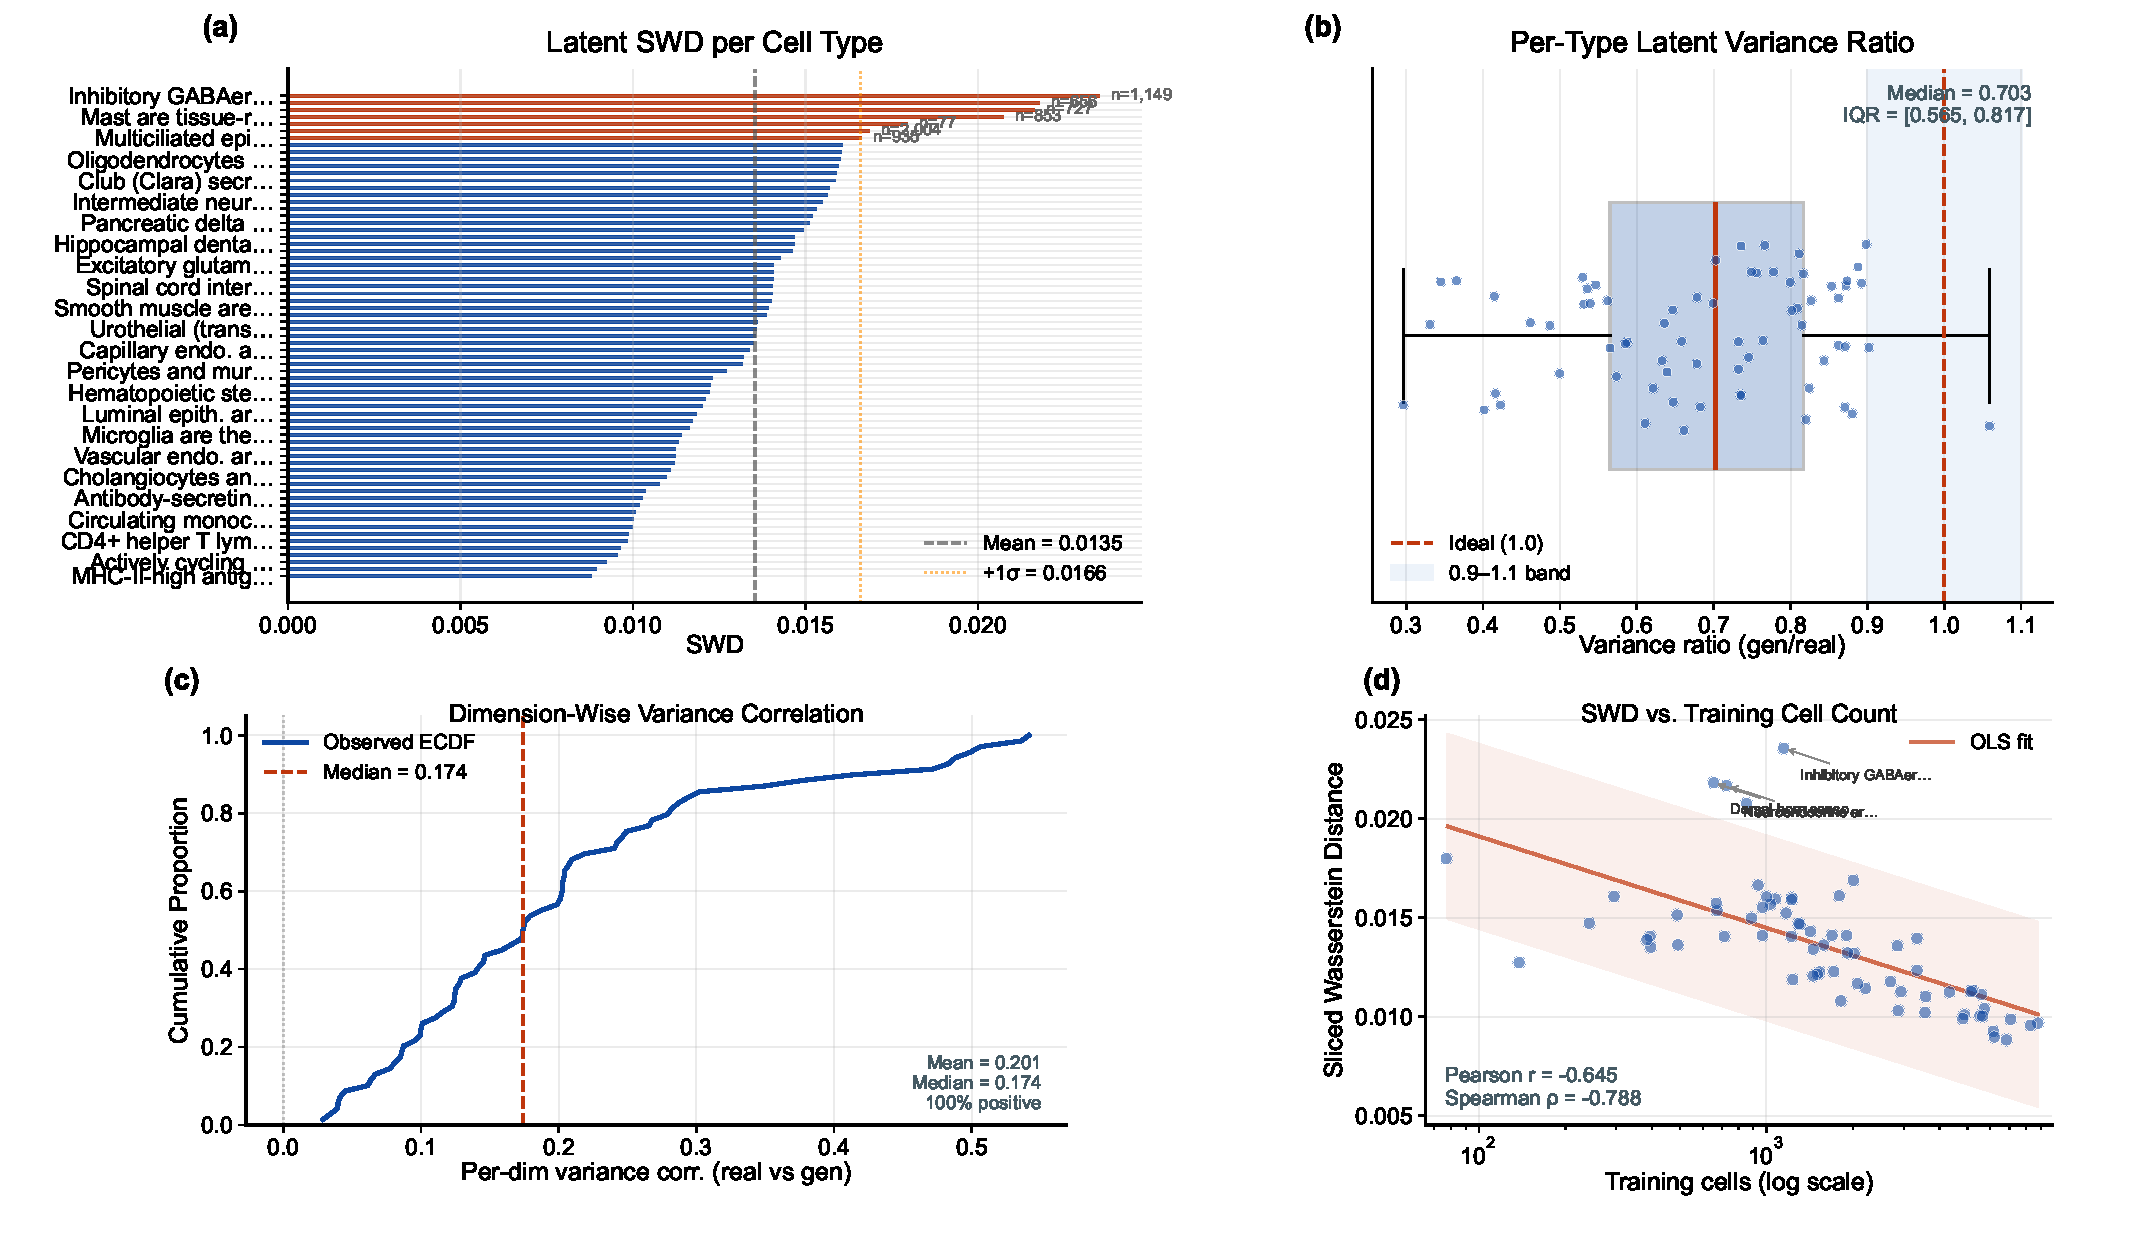
\includegraphics[width=0.95\textwidth]{figures/fig09a_variance_matching.pdf}\par\vspace{2pt}
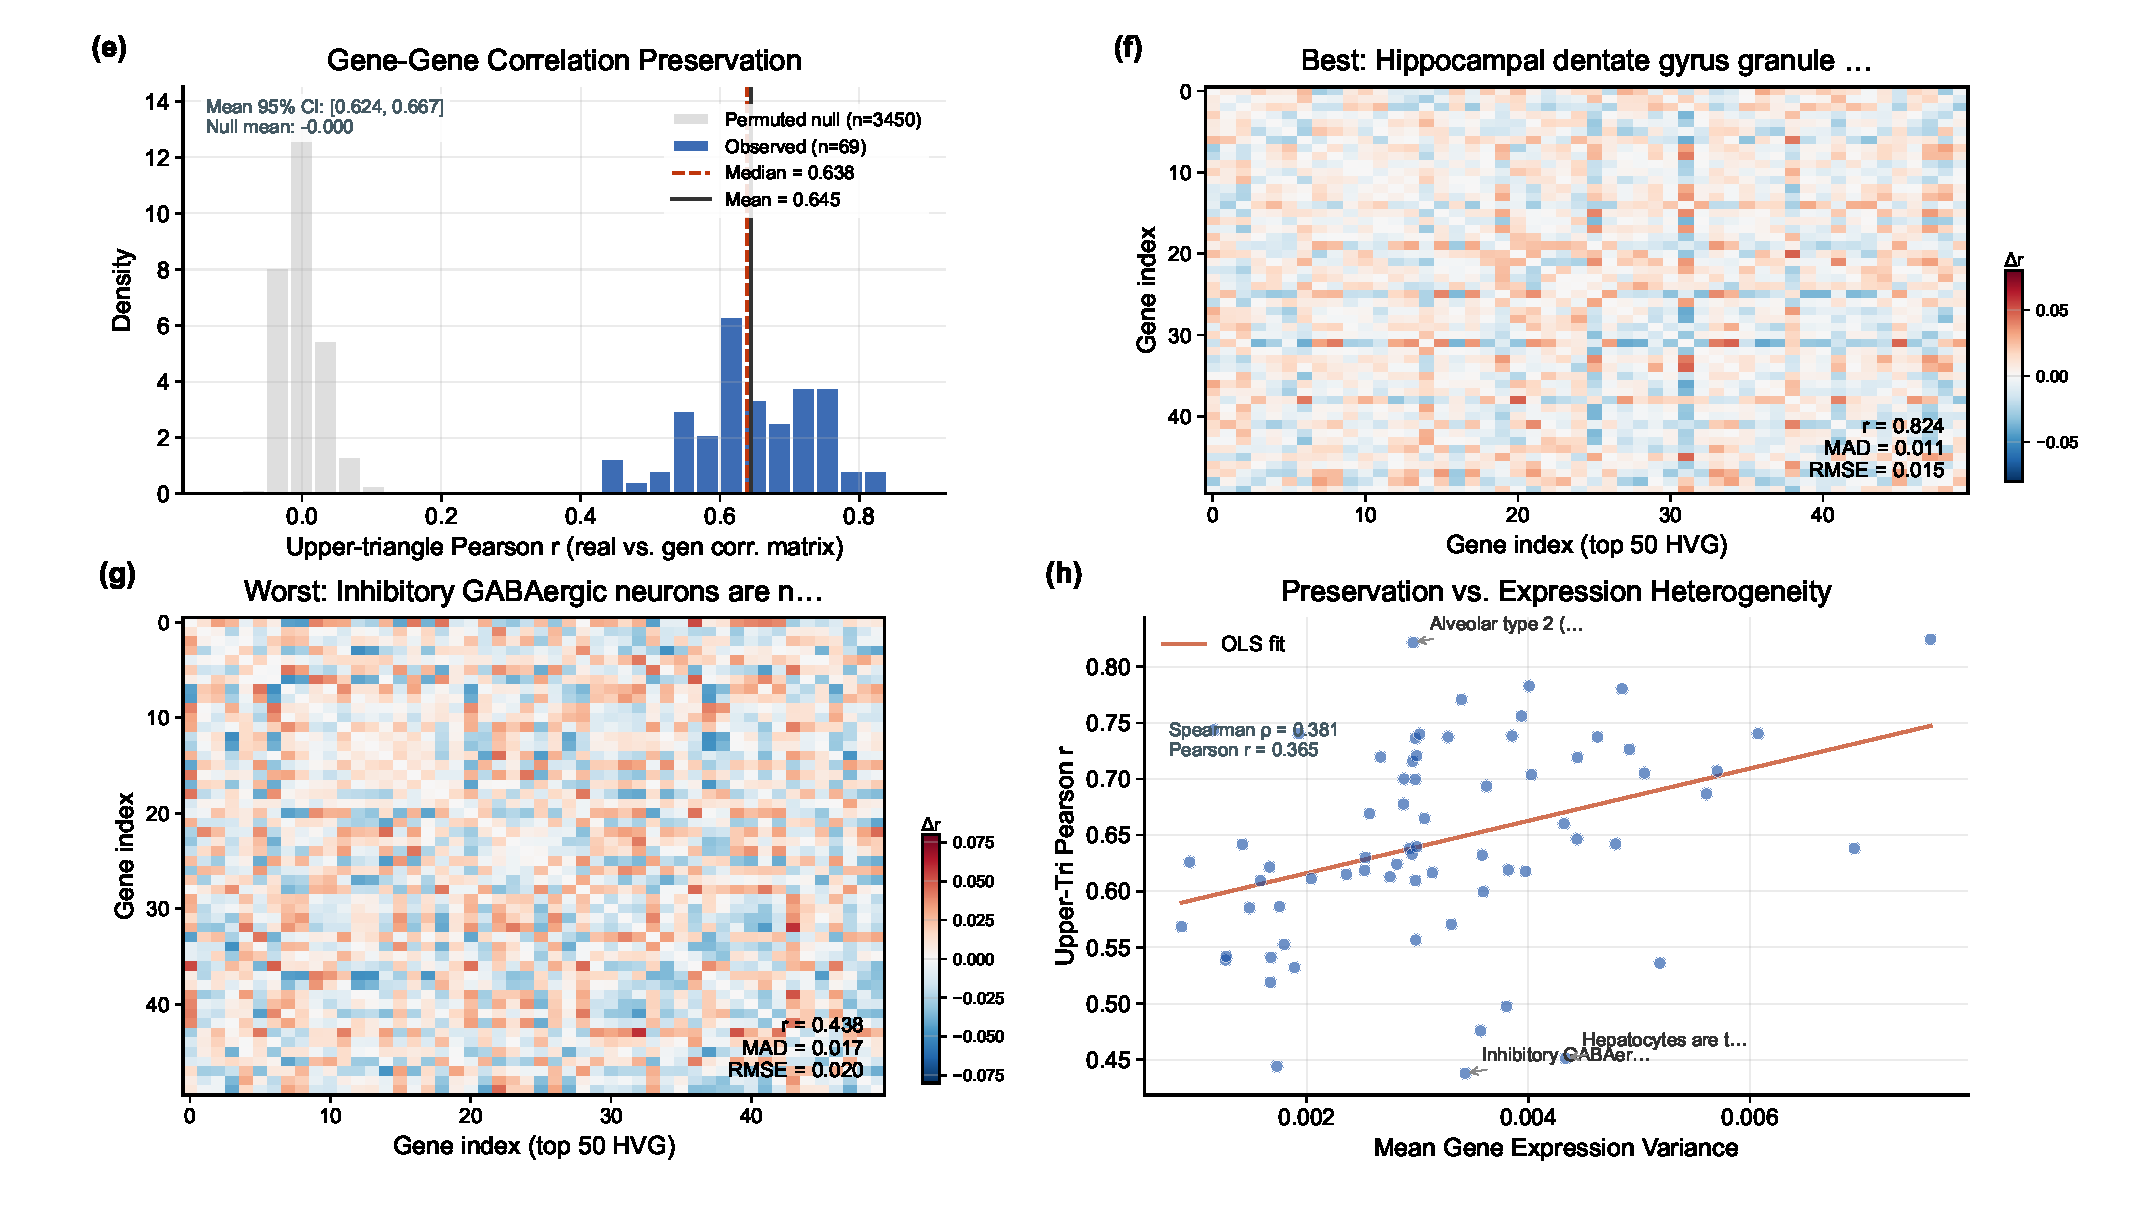
\includegraphics[width=0.95\textwidth]{figures/fig09b_gene_gene_correlation.pdf}
\caption{\textbf{Latent variance and gene--gene correlation analysis.} \emph{Variance matching} (\textbf{a})~Per-cell-type sliced Wasserstein distance (SWD) between real and generated latent distributions. (\textbf{b})~Per-type latent variance ratios (generated/real), summarized with the median and interquartile range relative to the ideal unity band. (\textbf{c})~Per-dimension variance-correlation ECDF, showing that most dimensions remain positively correlated but only weakly structured. (\textbf{d})~SWD versus training cell count with Pearson and Spearman trend summaries. \emph{Gene--gene correlation} (\textbf{e})~Distribution of per-type Mantel correlations with a permuted-null baseline overlay and bootstrap confidence interval on the mean preserved correlation. (\textbf{f--g})~Correlation-difference heatmaps for best- and worst-preserved cell types. (\textbf{h})~Mantel $r$ versus mean gene expression variance per type, showing only a weak dependence of preservation on intrinsic heterogeneity.\label{fig:var-pilot}\label{fig:gene-gene-corr}}
\end{figure}

\textbf{Ablation insights and reproducibility.} The CLOP ablation study (Figure~\ref{fig:ablation-heatmap}, Table~\ref{tab:ablation}) reveals a counterintuitive finding: removing cohesion and noise regularization \emph{improves} alignment accuracy by $+$10~pp, because these within-group tightening forces compete with inter-group separation when the base embedding space is near-degenerate. This suggests that regularization strategies for contrastive alignment should be tailored to the separation regime of the input embeddings. Multi-seed validation (Figure~\ref{fig:multi-seed}, Table~\ref{tab:multi-seed}) confirms low inter-run variance ($\sigma < 1$~pp for steering, $\sigma < 2$~pp for diversity ratio), indicating that the training procedure is stable despite the modest model size (25M total trainable parameters).

\textbf{Decoder bottleneck analysis.} Decoder ablations comparing frozen scGPT, LoRA-adapted, and MLP decoders produce broadly similar expression profiles (Appendix~\ref{app:suppl-figs}), indicating that the primary quality bottleneck lies upstream---in the latent generator and the geometry of the aligned embedding space---rather than in the decoder. This has practical implications: efforts to improve generation quality should focus on the alignment and flow-matching stages rather than on decoder engineering.

\textbf{Benchmarking and controllability.} On the nine distributional metrics shared by all methods, the Gaussian baseline outperforms CLOP-DiT (composite 0.747 vs.\ 0.694), showing that simple mean-matching is competitive when evaluation ignores conditioning. The distinctive value of CLOP-DiT is conditional controllability: CFG provides an interpretable fidelity--diversity knob, and the conditioning-field ablation demonstrates causal prompt dependence. This is the key architectural advantage over unconditional or weakly conditioned baselines.

\textbf{Limitations.} The 36.9\% KNN accuracy implies substantial residual class confusion in the tightly-packed embedding space; the high-fidelity regime (DivR = 0.513) is centroid-biased; and the rare-cell augmentation experiment was negative. All results are restricted to human and mouse cancer/developmental datasets. Expression-level agreement should be interpreted as a pipeline-level property (shared frozen decoder) rather than as evidence of faithful count-level reproduction.

\textbf{Modularity as a design principle.} The three-stage architecture enables independent improvement of each component. The aligner, generator, and decoder can be upgraded without retraining the full pipeline---for instance, replacing the scGPT decoder with a fine-tuned adapter, or substituting a stronger text encoder. This composability distinguishes CLOP-DiT from fully joint training approaches~\citep{ref-scdesign3} and positions it as a reusable framework for future work on conditioned generation in continuous latent spaces.

\section{Conclusions}\label{sec:conclusions}

We presented CLOP-DiT, a modular three-stage framework for structured-text-conditioned generation in continuous biological latent spaces. The pipeline combines prototype-aware contrastive alignment, 1D flow matching with group-aware regularization, and frozen foundation-model decoding. On 69 cell types from 80 datasets, the model achieves controllable generation with $25\times$-above-chance type specificity, reproducible operating regimes, and causal prompt dependence confirmed by ablation and permutation tests.

\textbf{Key technical findings.} (1)~PrototypeSigLIP alignment with ZCA whitening transforms near-degenerate embeddings (cosine similarity 0.994) into a well-separated condition space (0.222). (2)~Classifier-free guidance provides an interpretable fidelity--diversity trade-off. (3)~The quality bottleneck lies in the latent generator geometry, not the decoder. (4)~Group-aware variance regularization partially mitigates mean-collapse but does not solve it.

\textbf{Open problems.} Second-order structure preservation (variance, covariance) remains the primary unsolved challenge. The modular architecture provides a clear path forward: (i)~trajectory-level diversity objectives for the flow-matching stage; (ii)~decoder fine-tuning via LoRA~\citep{ref-scgpt} or lightweight adapters; (iii)~adaptive ODE solvers for improved distributional fidelity; (iv)~out-of-distribution evaluation on unseen cell types; and (v)~harmonized benchmarking against CellWhisperer~\citep{ref-cellwhisperer} and scDesign3~\citep{ref-scdesign3}. The composable design ensures each improvement can be tested independently without retraining the full pipeline.


\textbf{Data Availability.} The training and validation data were curated from publicly available GEO datasets; a full list of GEO accession identifiers is provided in Table~\ref{tab:s1_datasets} (Appendix~\ref{app:suppl-tables}), and the held-out validation study identifiers are in Table~\ref{tab:s2_validation}. Source code, trained model checkpoints (CLOP aligner and DiT generator), configuration files, environment specifications (Python~3.10, PyTorch~2.1, CUDA~12.0, scGPT~v0.2.1, Transformers~4.36), multi-seed validation data, independent marker gene validation data (PanglaoDB and CellMarker~2.0 cross-references), external marker ablation analysis, and one-command figure reproduction instructions are publicly available on GitHub~\citep{ref-clop-dit} and will be archived on Zenodo upon acceptance of this manuscript. All figures use colormaps designed for accessibility under common forms of color vision deficiency (deuteranopia, protanopia); critical distinctions additionally use shape or pattern encoding.

\textbf{Abbreviations.}
The following abbreviations are used in this manuscript:\\[4pt]
\begin{tabular}{@{}ll}
AdaLN & Adaptive Layer Normalization\\
CFG & Classifier-free guidance\\
CLOP & Contrastive Language-Omics Pretraining\\
DE & Differential expression\\
DiT & Diffusion Transformer\\
DivR & Diversity Ratio\\
EMA & Exponential Moving Average\\
FD & Fr\'{e}chet Distance\\
GEO & Gene Expression Omnibus\\
KNN & $k$-Nearest Neighbor\\
LinAcc & Linear Classifier Accuracy\\
logFC & Log Fold Change\\
LoRA & Low-Rank Adaptation\\
ODE & Ordinary Differential Equation\\
OOD & Out-of-Distribution\\
scGPT & Single-cell Generative Pre-trained Transformer\\
scRNA-seq & Single-cell RNA sequencing\\
SigLIP & Sigmoid Loss for Language-Image Pre-training\\
ZCA & Zero-phase Component Analysis
\end{tabular}

\FloatBarrier
\appendix
\section{Appendix A: Supplementary Material}\label{app:suppl-tables}\label{app:hyperparams}

\begin{table}[!htbp]
\caption{Architecture specifications.\label{tab:architecture}}
\centering
\begin{tabularx}{\textwidth}{lCC}
\toprule
\textbf{Component} & \textbf{Architecture} & \textbf{Parameters} \\
\midrule
BiomedBERT-large (frozen) & Transformer encoder  & 340M \\
CLOP text projector       & MLP [1024$\to$1024$\to$1024$\to$512] & 1.58M \\
CLOP cell projector       & MLP [512$\to$512$\to$512$\to$512]    & 1.44M \\
DiT1D                     & 8$\times$ AdaLN-Zero blocks, 8 heads & 22.10M \\
scGPT encoder (frozen)    & Transformer                          & $\sim$51M \\
scGPT decoder (frozen)    & Gene token prediction head           & included \\
\bottomrule
\end{tabularx}
\end{table}

\begin{table}[!htbp]
\caption{CFG scale sweep (10-step Euler, 69 eval groups). Values are computed on a different subsample (69 groups $\times$ 200 cells) than the primary operating-point results in Table~\ref{tab:core-results} (69 types $\times$ 200 cells with different random seeds), which accounts for minor numerical differences.\label{tab:cfg-sweep}}
\centering
\begin{tabular}{lrrrr}
\toprule
\textbf{CFG} & \textbf{KNN-1} & \textbf{Steering} & \textbf{DivR} & \textbf{KNN/Random} \\
\midrule
0.5 & 0.147 & 0.788 & 1.13 & 15$\times$ \\
1.0 & 0.348 & 0.796 & 0.76 & 35$\times$ \\
1.5 & 0.396 & 0.798 & 0.60 & 40$\times$ \\
2.0 & 0.407 & 0.806 & 0.53 & 41$\times$ \\
2.5 & 0.408 & 0.804 & 0.49 & 41$\times$ \\
3.0 & 0.410 & 0.802 & 0.48 & 41$\times$ \\
4.0 & 0.402 & 0.804 & 0.50 & 40$\times$ \\
5.0 & 0.380 & 0.798 & 0.55 & 38$\times$ \\
\bottomrule
\end{tabular}
\end{table}

\begin{table}[!htbp]
\caption{Training hyperparameters for both CLOP alignment and DiT flow-matching stages.\label{tab:hyperparams}}
\centering
\begin{tabularx}{\textwidth}{lCC}
\toprule
\textbf{Hyperparameter} & \textbf{CLOP} & \textbf{DiT} \\
\midrule
Optimizer         & AdamW              & AdamW ($\beta_1{=}0.9, \beta_2{=}0.999$) \\
Learning rate     & $5 \times 10^{-4}$ & $2 \times 10^{-4}$ \\
Weight decay      & 0.06               & 0.01 \\
Batch size        & 1024               & 1024 \\
Epochs            & 100                & 300 \\
Warmup epochs     & 5                  & 5 \\
LR schedule       & Cosine with warmup & Cosine with warmup \\
Gradient clipping  & 1.0               & 1.0 \\
Mixed precision   & FP16 (AMP)         & FP16 (AMP) \\
Dropout           & 0.2                & Proj: 0.1, Attn: 0.0 \\
EMA decay         & ---                & 0.9999 \\
Temperature       & 14.0 (fixed; see Section~\ref{sec:clop})       & --- \\
Loss              & PrototypeSigLIP    & Flow matching + variance/covariance regularization \\
Cohesion weight   & 0.15               & --- \\
Variance loss wt. & ---                & 0.10 \\
Covariance loss wt. & ---              & 0.05 \\
Label smoothing   & 0.1                & --- \\
CFG drop prob     & ---                & 0.15 \\
Time sampling     & ---                & Logit-normal ($\mu{=}0, \sigma{=}1$) \\
\bottomrule
\end{tabularx}
\end{table}

% Table S1: All 80 GEO Dataset Identifiers
{\footnotesize
\renewcommand{\arraystretch}{0.9}
\begin{longtable}{rllp{4.2cm}rr}
\caption{All 80 GEO datasets used in CLOP-DiT training and validation. Datasets were preprocessed to 2,000 highly variable genes per dataset. Split: Train or held-out Validation (study-level, seed 42). Hs: \textit{Homo sapiens}; Mm: \textit{Mus musculus}.\label{tab:s1_datasets}} \\
\toprule
\# & Accession & Organism & Description & $n_{\text{cells}}$ & Split \\
\midrule
\endfirsthead
\toprule
\# & Accession & Organism & Description & $n_{\text{cells}}$ & Split \\
\midrule
\endhead
\midrule
\multicolumn{6}{r}{\textit{Continued on next page}} \\
\endfoot
\bottomrule
\endlastfoot
  1 & GSE103867 & Hs & scRNA-seq (GEO-DataHub) & 2,787 & Val \\
  2 & GSE110686 & Hs & scRNA-seq (GEO-DataHub) & 2,992 & Train \\
  3 & GSE115571 & Mm & Mouse cells, LPS stimulation & 442 & Train \\
  4 & GSE117988 & Hs & PBMCs, Merkel cell carcinoma & 2,638 & Train \\
  5 & GSE117988 & Hs & Merkel cell carcinoma tumor & 2,990 & Train \\
  6 & GSE120505 & Hs & Aged blood cells & 3,000 & Train \\
  7 & GSE123813 & Hs & Basal cell carcinoma skin & 3,000 & Train \\
  8 & GSE123813 & Hs & Cutaneous squamous cell carcinoma & 3,000 & Train \\
  9 & GSE123902 & Hs & Lung adenocarcinoma & 2,753 & Train \\
  10 & GSE124310 & Hs & Multiple myeloma bone marrow & 2,833 & Train \\
  11 & GSE130148 & Hs & Fetal lung development & 3,000 & Train \\
  12 & GSE132509 & Hs & Pediatric ALL bone marrow & 2,984 & Train \\
  13 & GSE138709 & Hs & Intrahepatic cholangiocarcinoma & 2,891 & Train \\
  14 & GSE142653 & Hs & Pituitary gland development & 2,885 & Train \\
  15 & GSE143423 & Hs & Leptomeningeal brain metastasis & 3,000 & Train \\
  16 & GSE143423 & Hs & Triple-neg.\ breast cancer brain met. & 2,332 & Train \\
  17 & GSE145929 & Mm & Adult mouse prostate & 2,830 & Train \\
  18 & GSE145929 & Mm & Adult mouse urethra & 2,745 & Train \\
  19 & GSE148218 & Hs & Bone marrow, ALL & 2,807 & Train \\
  20 & GSE149655 & Hs & Early-stage lung adenocarcinoma & 2,087 & Train \\
  21 & GSE155109 & Hs & Endothelial cells, breast cancer & 3,000 & Train \\
  22 & GSE155109 & Hs & Stromal cells, breast cancer & 3,000 & Train \\
  23 & GSE163558 & Hs & Stomach cancer & 2,467 & Train \\
  24 & GSE165784 & Hs & Retina development & 2,622 & Train \\
  25 & GSE165844 & Mm & LSK hematopoietic progenitors & 2,881 & Train \\
  26 & GSE167597 & Mm & Mouse spinal cord development & 3,000 & Val \\
  27 & GSE168181 & Hs & Breast cancer tissue & 2,863 & Train \\
  28 & GSE175975 & Hs & scRNA-seq (GEO-DataHub) & 2,728 & Train \\
  29 & GSE183904 & Hs & Gastric cancer & 3,000 & Val \\
  30 & GSE189070 & Mm & Astrocytes, spinal cord injury & 2,960 & Train \\
  31 & GSE189357 & Hs & Lung adenocarcinoma & 2,886 & Train \\
  32 & GSE192857 & Hs & hESC differentiation time-series & 2,696 & Train \\
  33 & GSE212502 & Hs & Forebrain organoids & 3,000 & Train \\
  34 & GSE213740 & Hs & Ascending aortic wall dissection & 2,704 & Val \\
  35 & GSE220913 & Hs & HL-60 cell lines, CFTR & 2,972 & Train \\
  36 & GSE222002 & Hs & T cells from cancer & 2,962 & Train \\
  37 & GSE222369 & Hs & NK cells, lymphoma & 2,778 & Train \\
  38 & GSE225600 & Hs & Breast cancer tumor & 2,333 & Train \\
  39 & GSE225857 & Hs & Colorectal cancer liver metastases & 2,986 & Train \\
  40 & GSE226131 & Mm & Aged hematopoietic stem cells & 2,608 & Train \\
  41 & GSE226762 & Hs & scRNA-seq (GEO-DataHub) & 830 & Val \\
  42 & GSE227644 & Hs & scRNA-seq (GEO-DataHub) & 3,000 & Train \\
  43 & GSE227719 & Mm & KrasG12D/P53 lung organoids & 2,990 & Train \\
  44 & GSE228499 & Hs & Breast cancer & 2,448 & Train \\
  45 & GSE235787 & Hs & B cells, ALL & 2,798 & Train \\
  46 & GSE236565 & Mm & Splenic CD4+ T cells & 2,556 & Train \\
  47 & GSE248214 & Hs & scRNA-seq (GEO-DataHub) & 2,998 & Train \\
  48 & GSE253355 & Hs & Bone marrow niche & 2,835 & Train \\
  49 & GSE262288 & Hs & Metastatic breast cancer & 2,321 & Train \\
  50 & GSE272187 & Hs & scRNA-seq (GEO-DataHub) & 2,639 & Train \\
  51 & GSE275119 & Mm & Dental tissue development & 2,963 & Train \\
  52 & GSE277740 & Mm & Thalamus, SBS vs DNBSEQ & 2,644 & Val \\
  53 & GSE279781 & Hs & scRNA-seq (GEO-DataHub) & 2,654 & Train \\
  54 & GSE280847 & Mm & CD45+ leukocytes, MC38 tumor & 2,864 & Train \\
  55 & GSE283205 & Hs & Hepatoblastoma tumor tissue & 2,994 & Train \\
  56 & GSE283397 & Hs & CD8+ T cells, CLL & 2,856 & Train \\
  57 & GSE288211 & Mm & Pancreatic islets, Zzef1 KO & 2,724 & Train \\
  58 & GSE289611 & Hs & Pulmonary pleomorphic carcinoma & 2,983 & Train \\
  59 & GSE291166 & Mm & Mesenteric lymph node & 2,901 & Train \\
  60 & GSE299623 & Hs & scRNA-seq (GEO-DataHub) & 2,991 & Train \\
  61 & GSE300862 & Mm & Kras/Trp53 lung adenocarcinoma & 2,716 & Val \\
  62 & GSE302433 & Mm & B16F10 melanoma, ZDHHC13 & 2,953 & Val \\
  63 & GSE303309 & Mm & Brain CD45+ immune cells, AD & 2,999 & Train \\
  64 & GSE306567 & Mm & ESCs and neural progenitors & 2,454 & Train \\
  65 & GSE306676 & Mm & Spinal cord, SOD1-G93A ALS & 2,959 & Train \\
  66 & GSE307261 & Hs & B and T cells, melanoma & 2,921 & Train \\
  67 & GSE307774 & Mm & Colorectal tumors, Kras/Braf & 2,505 & Train \\
  68 & GSE308428 & Mm & Hippocampal microglia, ASD & 2,991 & Train \\
  69 & GSE309368 & Hs & Myeloid cells, oral SCC & 1,361 & Train \\
  70 & GSE315628 & Mm & scRNA-seq (GEO-DataHub) & 2,895 & Train \\
  71 & GSE318353 & Hs & scRNA-seq (GEO-DataHub) & 2,964 & Train \\
  72 & GSE98638  & Hs & HCC T cell landscape & 3,000 & Train \\
  73 & GSE120446 & Hs & Bone marrow, hematopoietic dev. & 2,890 & Train \\
  74 & GSE104323 & Mm & Dentate gyrus, brain development & 3,000 & Train \\
  75 & GSE75748  & Hs & Endoderm differentiation & 2,531 & Train \\
  76 & GSE144024 & Hs & Human embryonic stem cells & 3,000 & Train \\
  77 & GSE72857  & Mm & Hematopoiesis & 3,000 & Train \\
  78 & GSE226824 & Hs & IFN-treated HSPCs & 2,739 & Train \\
  79 & GSE141259 & Mm & Lung development & 3,000 & Train \\
  80 & GSE139369 & Hs & Hematopoiesis (Setty et al.) & 2,995 & Train \\
\midrule
  & \textbf{Total} & & & \textbf{220,304} & \\
\end{longtable}
}% end footnotesize for Table S1

% Table S2: 8 Held-out Validation Datasets
\begin{table}[!htbp]
\centering
\caption{The 8 held-out validation datasets (study-level split, seed 42, val\_split = 0.1). No cells from these studies were seen during CLOP or DiT training. Hs: \textit{Homo sapiens}; Mm: \textit{Mus musculus}.\label{tab:s2_validation}}
\begin{tabular}{rllp{4.5cm}r}
\toprule
\# & Accession & Organism & Description & $n_{\text{cells}}$ \\
\midrule
  1 & GSE103867 & Hs & scRNA-seq (GEO-DataHub) & 2,787 \\
  2 & GSE167597 & Mm & Mouse spinal cord development & 3,000 \\
  3 & GSE183904 & Hs & Gastric cancer & 3,000 \\
  4 & GSE213740 & Hs & Ascending aortic wall dissection & 2,704 \\
  5 & GSE226762 & Hs & scRNA-seq (GEO-DataHub) & 830 \\
  6 & GSE277740 & Mm & Thalamus, SBS vs DNBSEQ & 2,644 \\
  7 & GSE300862 & Mm & Kras/Trp53 lung adenocarcinoma & 2,716 \\
  8 & GSE302433 & Mm & B16F10 melanoma, ZDHHC13 & 2,953 \\
\midrule
  & \textbf{Total} & & \textbf{20,634} \\
\bottomrule
\end{tabular}
\end{table}

% Table S3: Full CFG Scale / Solver / Steps Sweep Results
{\footnotesize
\renewcommand{\arraystretch}{0.9}
\begin{longtable}{lllrrrrrr}
\caption{Full CFG scale sweep. 200 cells generated per group (69 groups). KNN: type-identity accuracy; Steer.: alignment; DivR: diversity ratio (1.0 = ideal); LinAcc: linear classifier accuracy; FD: Fr\'{e}chet distance.\label{tab:s3_cfg_sweep}} \\
\toprule
CFG & Solver & Steps & KNN-1 & KNN-5 & Steer. & DivR & LinAcc & FD \\
\midrule
\endfirsthead
\toprule
CFG & Solver & Steps & KNN-1 & KNN-5 & Steer. & DivR & LinAcc & FD \\
\midrule
\endhead
\midrule
\multicolumn{9}{r}{\textit{Continued on next page}} \\
\endfoot
\bottomrule
\endlastfoot
\multicolumn{9}{l}{\textit{Primary configurations (Table~\ref{tab:core-results})}} \\
\midrule
  3.0 & Euler & 10 & 0.367 & 0.554 & 0.802 & 0.473 & 0.508 & 3.46 \\
  2.0 & Euler & 10 & 0.369 & 0.553 & 0.810 & 0.513 & 0.511 & 3.17 \\
  1.0 & Euler & 10 & 0.313 & 0.483 & 0.810 & 0.745 & 0.390 & 2.84 \\
  0.0 & Euler & 10 & 0.010 & 0.051 & 0.475 & 1.833 & 0.010 & 0.58 \\
  3.0 & Midpoint & 10 & 0.340 & 0.528 & 0.792 & 0.628 & 0.477 & 3.38 \\
  2.0 & Midpoint & 10 & 0.340 & 0.525 & 0.800 & 0.686 & 0.475 & 3.13 \\
  1.0 & Midpoint & 10 & 0.288 & 0.461 & 0.807 & 0.929 & 0.357 & 2.64 \\
  3.0 & Euler & 50 & 0.348 & 0.545 & 0.795 & 0.622 & 0.489 & 3.33 \\
  1.0 & Euler & 50 & 0.293 & 0.466 & 0.807 & 0.919 & 0.365 & 2.65 \\
  --- & Gaussian & --- & 0.011 & 0.048 & 0.466 & 2.277 & 0.009 & 0.03 \\
\midrule
\multicolumn{9}{l}{\textit{Fine-grained CFG sweep (Euler solver)}} \\
\midrule
  0.5 & Euler & 10 & 0.147 & 0.284 & 0.788 & 1.129 & --- & 2.33 \\
  1.0 & Euler & 10 & 0.348 & 0.515 & 0.796 & 0.757 & --- & 2.94 \\
  1.5 & Euler & 10 & 0.396 & 0.553 & 0.798 & 0.600 & --- & 3.36 \\
  2.0 & Euler & 10 & 0.407 & 0.580 & 0.806 & 0.526 & --- & 3.54 \\
  2.5 & Euler & 10 & 0.408 & 0.590 & 0.804 & 0.493 & --- & 3.70 \\
  3.0 & Euler & 10 & 0.410 & 0.592 & 0.802 & 0.484 & --- & 3.80 \\
  4.0 & Euler & 10 & 0.402 & 0.586 & 0.804 & 0.502 & --- & 4.01 \\
  5.0 & Euler & 10 & 0.380 & 0.576 & 0.798 & 0.548 & --- & 4.34 \\
  0.5 & Euler & 20 & 0.137 & 0.269 & 0.788 & 1.230 & --- & 2.07 \\
  1.0 & Euler & 20 & 0.334 & 0.504 & 0.794 & 0.842 & --- & 2.83 \\
  1.5 & Euler & 20 & 0.380 & 0.545 & 0.798 & 0.679 & --- & 3.19 \\
  2.0 & Euler & 20 & 0.391 & 0.569 & 0.798 & 0.600 & --- & 3.43 \\
  2.5 & Euler & 20 & 0.394 & 0.578 & 0.800 & 0.559 & --- & 3.66 \\
  3.0 & Euler & 20 & 0.398 & 0.582 & 0.800 & 0.540 & --- & 3.77 \\
  4.0 & Euler & 20 & 0.388 & 0.578 & 0.802 & 0.535 & --- & 3.97 \\
  5.0 & Euler & 20 & 0.379 & 0.567 & 0.792 & 0.551 & --- & 4.16 \\
  0.5 & Euler & 50 & 0.132 & 0.259 & 0.792 & 1.318 & --- & 1.95 \\
  1.0 & Euler & 50 & 0.324 & 0.495 & 0.794 & 0.933 & --- & 2.72 \\
  1.5 & Euler & 50 & 0.370 & 0.538 & 0.796 & 0.776 & --- & 3.14 \\
  2.0 & Euler & 50 & 0.384 & 0.563 & 0.796 & 0.699 & --- & 3.31 \\
  2.5 & Euler & 50 & 0.388 & 0.576 & 0.796 & 0.658 & --- & 3.48 \\
  3.0 & Euler & 50 & 0.392 & 0.581 & 0.792 & 0.637 & --- & 3.64 \\
  4.0 & Euler & 50 & 0.379 & 0.579 & 0.790 & 0.622 & --- & 3.86 \\
  5.0 & Euler & 50 & 0.378 & 0.570 & 0.790 & 0.626 & --- & 4.10 \\
\end{longtable}
}% end footnotesize for Table S3

% Table S4: 5 Biological Validation Datasets
\begin{table}[!htbp]
\centering
\caption{The 5 biological validation datasets used for marker gene correlation, expression distribution fidelity, and Gene Ontology enrichment analysis (Section~\ref{sec:cross-dataset}). These datasets were selected to span diverse human cancer tissue types and immune cell populations. \textbf{Four of the five datasets are from the training split; only GSE183904 is held-out (Table~S2). This analysis therefore primarily evaluates in-distribution decoder-reconstructed fidelity, not out-of-distribution generalization.}}
\label{tab:s4_biovalidation}
\small
\begin{tabularx}{\textwidth}{rllXcr}
\toprule
\# & Accession & Tissue & Description & Split & $n_{\text{cells}}$ \\
\midrule
  1 & GSE123902 & Lung & Lung adenocarcinoma TME & Train & 2,753 \\
  2 & GSE183904 & Gastric & Gastric cancer TME & Val & 3,000 \\
  3 & GSE123813 & Skin & Basal cell carcinoma & Train & 3,000 \\
  4 & GSE98638 & Liver & HCC T cell landscape & Train & 3,000 \\
  5 & GSE132509 & Blood & ALL bone marrow cells & Train & 2,984 \\
\midrule
  & \textbf{Total} & & & & \textbf{14,737} \\
\bottomrule
\end{tabularx}
\vspace{4pt}
{\footnotesize All datasets are \textit{Homo sapiens}. Validation purpose for each: marker gene correlation, expression distribution fidelity, and GO enrichment.}
\end{table}

% Table S5: Bootstrap 95% Confidence Intervals
\begin{table}[!htbp]
\centering
\caption{Bootstrap 95\% confidence intervals (percentile method, $B{=}1{,}000$) for headline generation metrics. Resampling unit: cell types ($n{=}69$ types resampled with replacement). Classifiers (KNN, logistic regression) were trained once on real data; only the composition of evaluated types varies across bootstrap iterations. Generation configuration: CFG\,=\,1.5, Midpoint solver, 20 steps. Point estimates reflect the full (non-resampled) evaluation over all 69 types (100 generated cells per type, 6,900 total).}
\label{tab:s5_bootstrap_ci}
\begin{tabular}{lrrrr}
\toprule
Metric & Point Est. & 95\% CI Lower & 95\% CI Upper & Boot.\ SE \\
\midrule
KNN Top-1 Accuracy      & 0.509 & 0.421 & 0.586 & 0.043 \\
KNN Top-5 Accuracy      & 0.728 & 0.658 & 0.794 & 0.035 \\
Steering Accuracy       & 1.000 & 1.000 & 1.000 & 0.000 \\
Diversity Ratio (DivR)  & 0.969 & 0.963 & 0.974 & 0.003 \\
Linear Classifier Acc.  & 0.583 & 0.518 & 0.646 & 0.034 \\
Centroid Cosine Sim.    & 0.898 & 0.875 & 0.913 & 0.009 \\
\bottomrule
\end{tabular}
\end{table}

\subsection{Supplementary Figures}\label{app:suppl-figs}

\begin{figure}[p]
\centering
\makebox[\textwidth][c]{%
  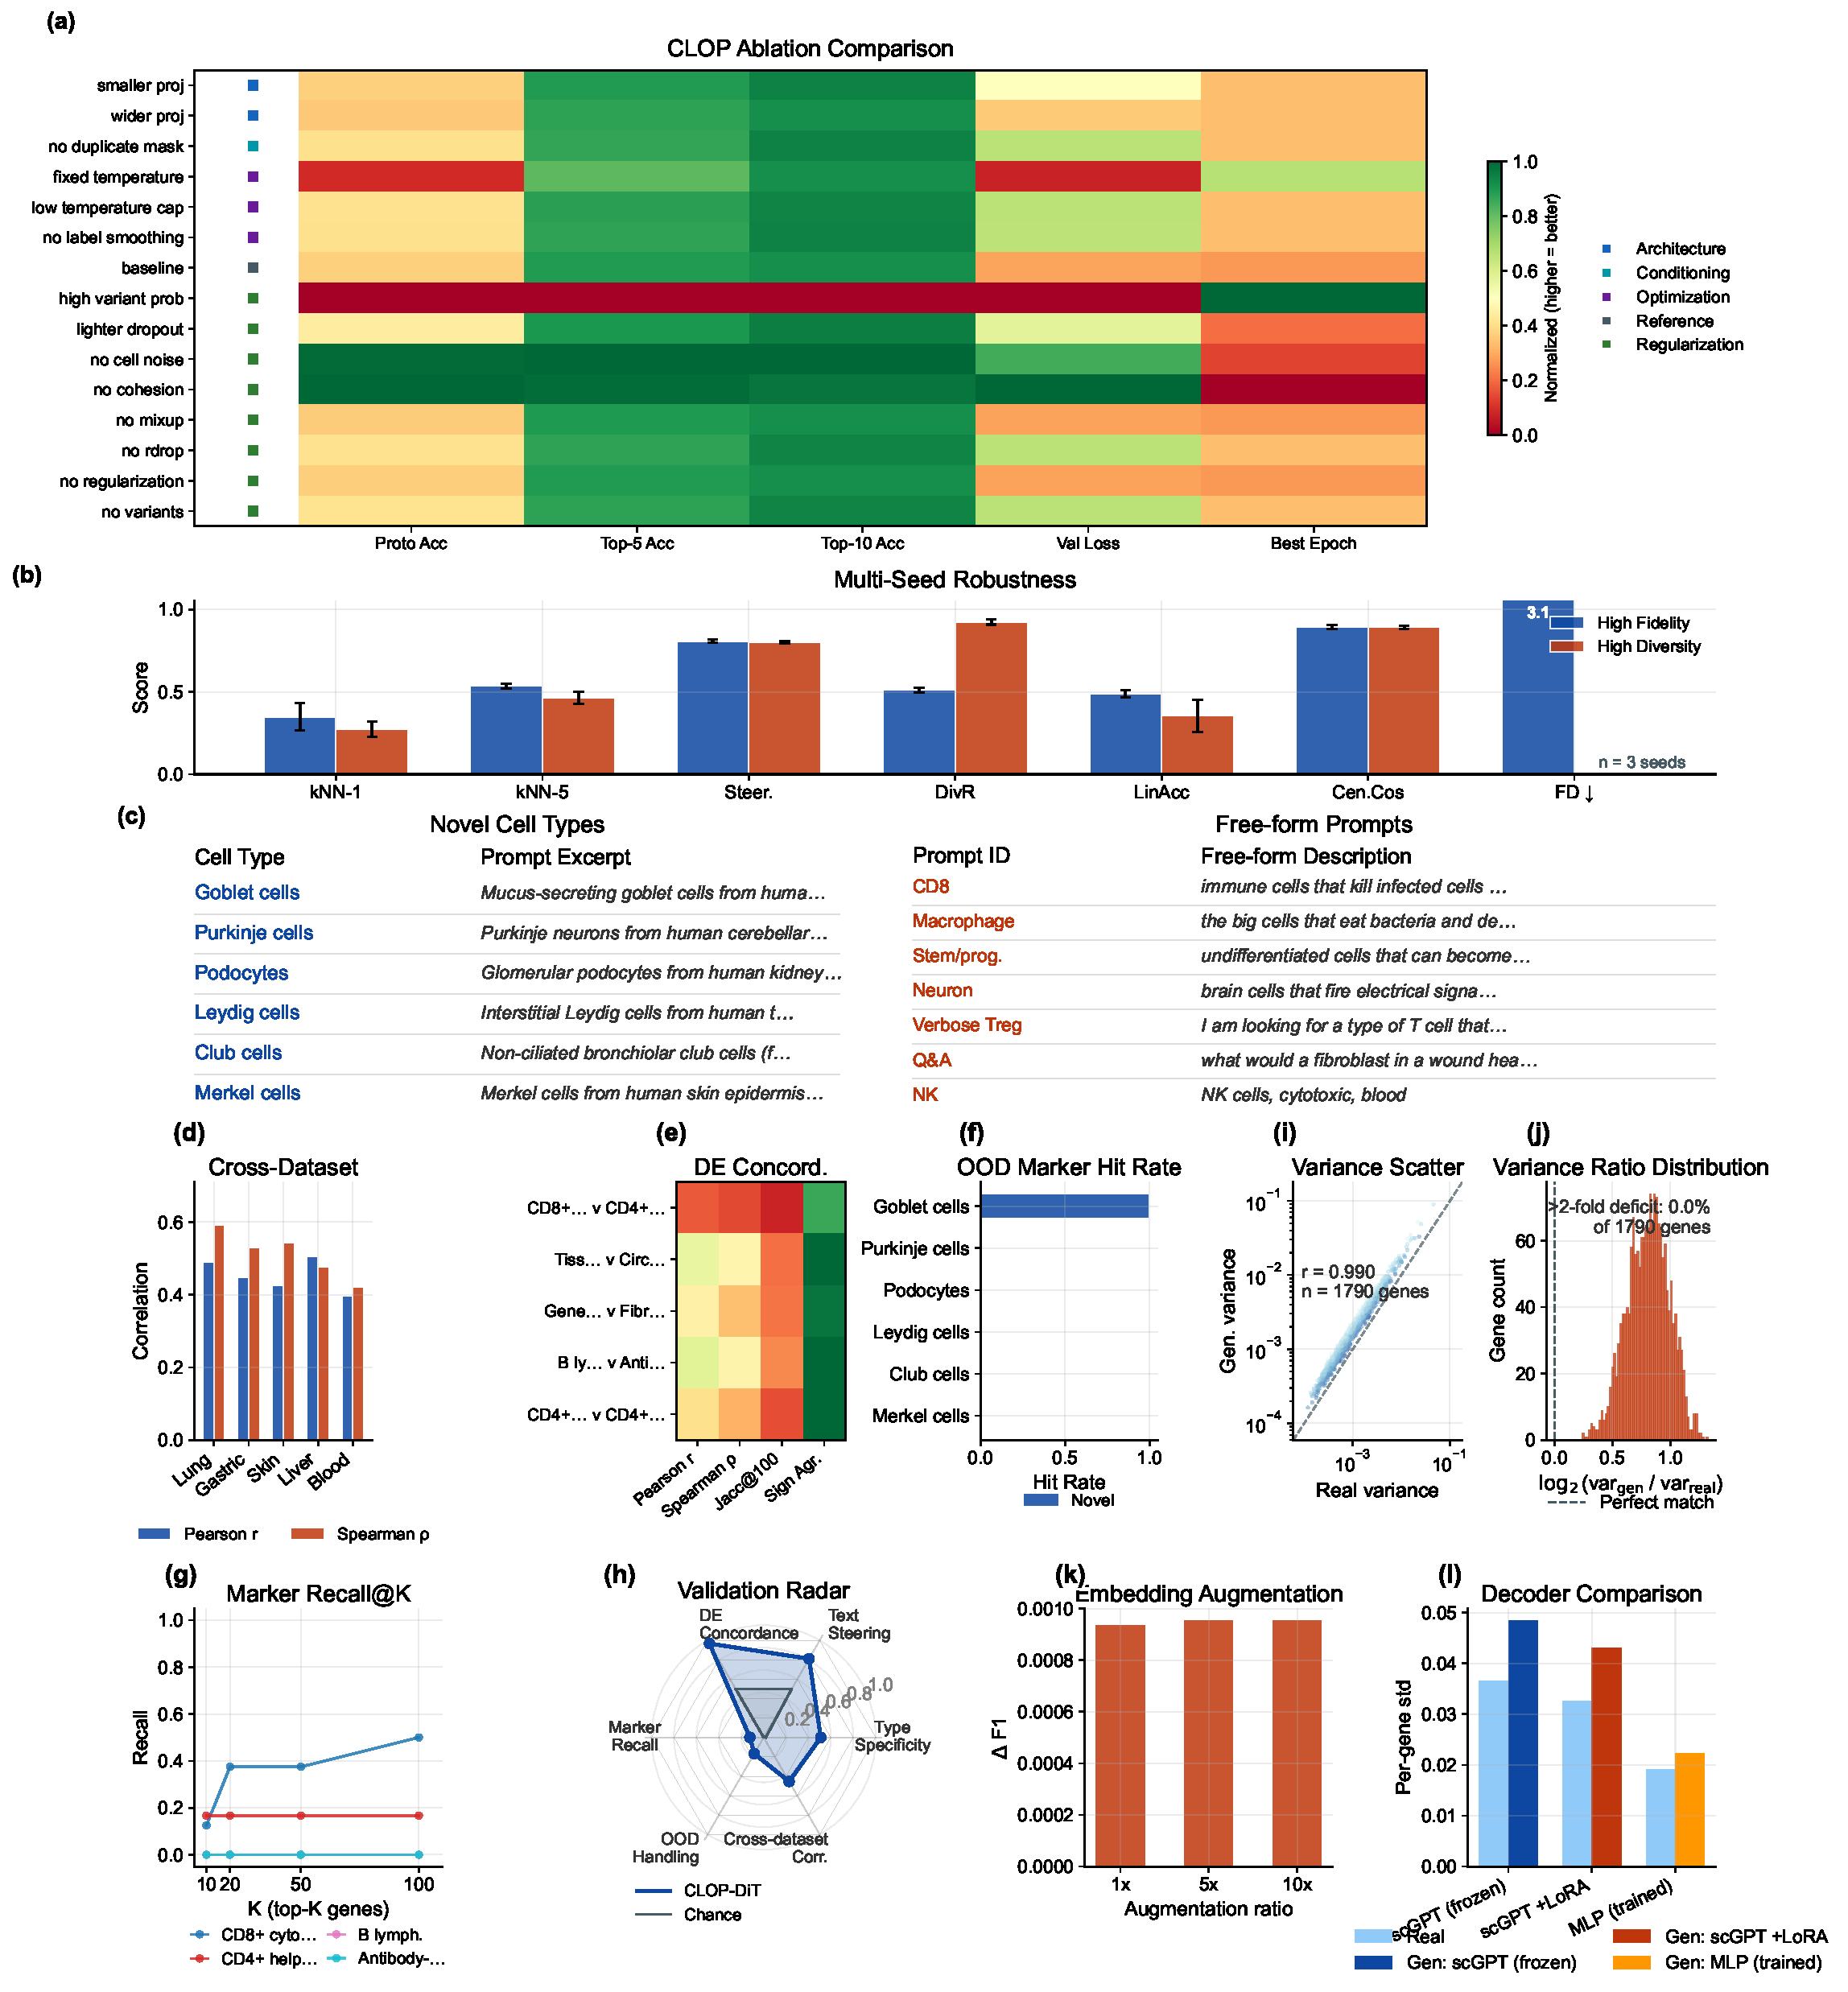
\includegraphics[width=1.15\textwidth,keepaspectratio]{figures/figS01_supplementary_validation.pdf}%
}
\caption{\textbf{Supplementary validation, ablation, and expression fidelity.}
\textbf{(a--c)}~Robustness and ablation: (a)~CLOP ablation heatmap showing normalised metrics across 15 configuration variants with component-category markers, (b)~multi-seed generation robustness across the high-fidelity and high-diversity operating regimes ($n = 3$ independent seeds), and (c)~out-of-distribution generation showcase listing six novel cell types (unseen during training) and eight free-form natural-language prompts.
\textbf{(d--h)}~Downstream validation suite: (d)~cross-dataset mean-expression correlation (Pearson~$r$ and Spearman~$\rho$) across five held-out tissues, (e)~expanded differential-expression concordance heatmap across five cell-type contrasts, (f)~OOD marker-hit rates for novel cell types, (g)~marker recall@$K$ curves for six representative cell types, and (h)~six-axis validation radar summarising type specificity, text steering, DE concordance, marker recall, OOD handling, and cross-dataset correlation.
\textbf{(i--l)}~Expression fidelity and decoder analysis: (i)~per-gene variance scatter (log-log scale) between real and generated profiles, (j)~variance-ratio distribution highlighting the fraction of genes with $>$2-fold deficit, (k)~embedding-level augmentation $\Delta$F1 at 1$\times$, 5$\times$, and 10$\times$ ratios, and (l)~decoder ablation comparing frozen scGPT, LoRA-adapted scGPT, and a trained MLP decoder.\label{fig:ablation-heatmap}\label{fig:multi-seed}\label{fig:ood-showcase}\label{fig:cross-dataset}\label{fig:expanded-de}\label{fig:ood-robustness}\label{fig:marker-completeness}\label{fig:validation-summary}\label{fig:variance-deepdive}\label{fig:embedding-augmentation}\label{fig:decoder-ablation}}
\end{figure}

\begin{figure}[p]
\centering
\makebox[\textwidth][c]{%
  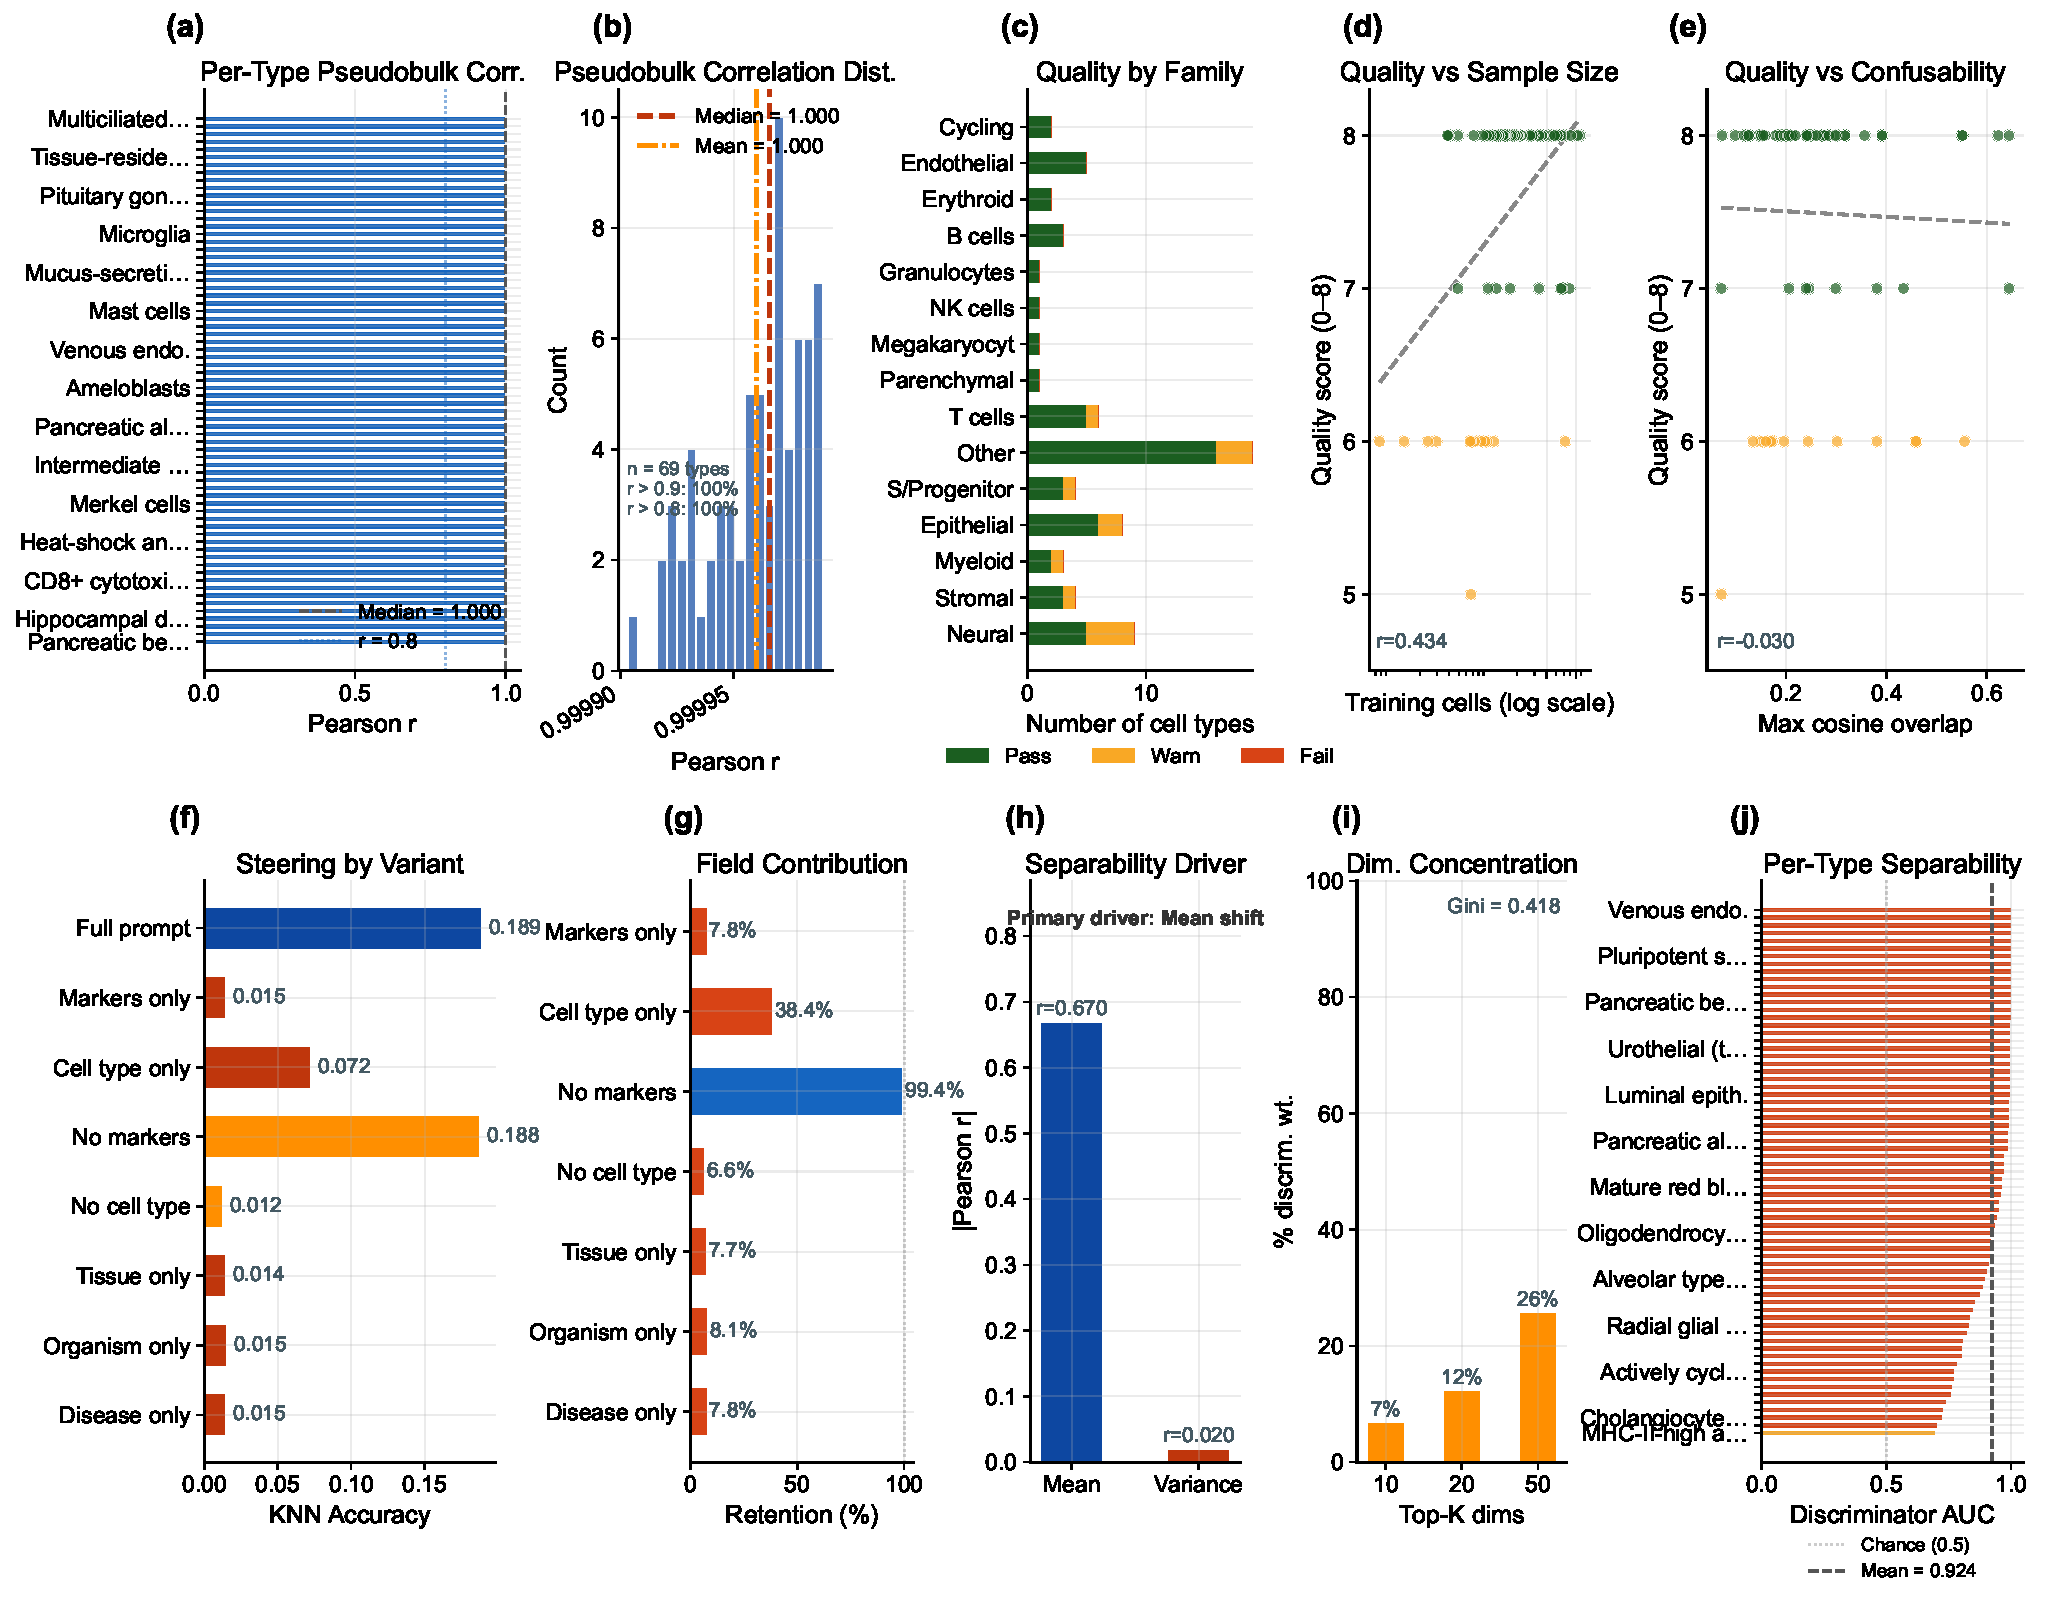
\includegraphics[width=1.25\textwidth,keepaspectratio]{figures/figS02_expression_diagnostics.pdf}%
}
\caption{\textbf{Expression-level validation and diagnostic analyses.}
\textbf{(a,\,b)}~Per-cell-type pseudobulk correlation between real and generated mean-expression profiles ($n = 69$ types): (a)~sorted Pearson~$r$ per type and (b)~distribution of correlations with median and mean indicators.
\textbf{(c--e)}~Failure-mode analysis: (c)~quality-tier distribution (pass/warn/fail) stratified by biological family, (d)~quality score versus training sample size (Pearson~$r = 0.43$), and (e)~quality score versus embedding confusability (Pearson~$r = -0.03$), indicating that generation quality scales with data abundance but is robust to inter-type similarity.
\textbf{(f,\,g)}~Prompt-field ablation: (f)~per-variant KNN accuracy showing that the cell-type field dominates steering effectiveness, and (g)~retention relative to the full prompt (cell type alone retains 38\,\%; removing the cell type drops accuracy to 7\,\%).
\textbf{(h--j)}~Discriminator feature importance: (h)~separability is primarily mean-driven ($|r| = 0.67$) rather than variance-driven, (i)~discriminative-weight concentration across embedding dimensions (Gini coefficient = 0.42), and (j)~per-type real-versus-generated AUC distribution (mean AUC = 0.92).\label{fig:pseudobulk}\label{fig:failure-analysis}\label{fig:field-ablation}\label{fig:discriminator}}
\end{figure}

\FloatBarrier



\section*{CRediT authorship contribution statement}

\textbf{Zeyu Fu}: Conceptualization, Methodology, Software, Validation, Formal analysis, Investigation, Resources, Data curation, Writing -- original draft, Writing -- review \& editing, Visualization, Supervision, Project administration, Funding acquisition.
\textbf{JianXu Zheng}: Writing -- review \& editing, Validation.
\textbf{Jiawei Fu}: Writing -- review \& editing, Validation.

\section*{Declaration of competing interest}

The authors declare no conflicts of interest.

\section*{Acknowledgments}

The authors acknowledge the developers and communities behind scGPT, BiomedBERT, and the Gene Expression Omnibus (GEO) for providing open-access tools and datasets that made this work possible. This work was supported by the National Key Research and Development Program of China (Grant No.~2024YFA1107101), the Ministry of Science and Technology of the People's Republic of China, and the National Key Laboratory of Trauma and Chemical Poisoning (Grant No.~2024K004).

AI-assisted tools (including Claude and GitHub Copilot) were used for code development (pipeline implementation, figure generation scripts, and evaluation infrastructure), manuscript drafting assistance, and language editing. All AI-generated content was reviewed, verified, and revised by the authors, who take full responsibility for the accuracy and integrity of the manuscript. No AI tools were used for data collection, experimental design, or interpretation of results.

\section*{Ethics statement}

Ethical review and approval were waived for this study, as only publicly available, de-identified data from the Gene Expression Omnibus (GEO) were analyzed. No new human subjects research, animal experiments, or clinical interventions were conducted. Informed consent was not applicable.

\section*{Data availability}

The training and validation data were curated from publicly available GEO datasets; a full list of GEO accession identifiers is provided in Table~\ref{tab:s1_datasets} (Appendix~\ref{app:suppl-tables}), and the held-out validation study identifiers are in Table~\ref{tab:s2_validation}. Source code, trained model checkpoints, configuration files, environment specifications, and one-command figure reproduction instructions are publicly available on GitHub \citep{ref-clop-dit} and will be archived on Zenodo upon acceptance. All figures use colormaps designed for accessibility under common forms of color vision deficiency.

\bibliographystyle{elsarticle-harv}
\bibliography{references}

\end{document}
